% PASTE INTO report_main.tex
% Compile with: pdflatex report_main.tex → bibtex report_main → pdflatex report_main → pdflatex report_main
\documentclass[14pt,a4paper]{extarticle}

% ── PACKAGES ──────────────────────────────────────────────────────────────────
\usepackage[left=3cm, right=1.5cm, top=2cm, bottom=2cm]{geometry}
\usepackage{setspace}\onehalfspacing
\usepackage{mathptmx} % Times New Roman font
\usepackage{fontenc}
\usepackage{inputenc}
\usepackage[hidelinks]{hyperref}
\usepackage{amsmath}
\usepackage{booktabs}
\usepackage{longtable}
\usepackage{graphicx}
\usepackage{caption}
\usepackage{subcaption}
\usepackage{float}
\usepackage{natbib} % author-year citations
\usepackage{xcolor}
\usepackage{titlesec}
\usepackage{abstract}
\usepackage{fancyhdr}
\usepackage{appendix}

\pagestyle{fancy}
\fancyhf{}
\rhead{\small NE Asian GVC Integration and Uzbekistan Industrialisation}
\cfoot{\thepage}


\begin{document}
\thispagestyle{empty}



% ── ABSTRACT ──────────────────────────────────────────────────────────────────
\begin{abstract}
\noindent This paper examines Uzbekistan's integration into Northeast Asian production networks following the 2017 Mirziyoyev reforms, demonstrating a central structural asymmetry: Uzbekistan has achieved significant backward global value chain (GVC) integration by absorbing intermediate goods, but has failed to achieve commensurate forward integration into manufactured export markets. This pattern signifies a captive rather than relational GVC governance structure. Employing a Chow structural break test, revealed comparative advantage indices, and bilateral trade decomposition, the analysis confirms that the 2017 reforms constituted a statistically significant turning point for manufacturing value added ($F=6.937$, $p=0.013$), accelerating annual sector growth from 0.4 to 1.2 percentage points. Data span 2010--2026, with 2024--2026 drawn from IMF WEO April 2025 projections. However, a persistent gap in foreign direct investment (FDI) intensity remains, particularly compared to Vietnam's post-2000 trajectory. Crucially, the type of capital flowing into Uzbekistan deviates from the export-manufacturing focus predicted by the flying geese model; the country disproportionately attracts infrastructure-linked Chinese FDI, whereas export-oriented Japanese and South Korean manufacturing FDI remains marginal despite high intermediate-goods trade shares. The dissertation argues that escaping this captive integration trap requires shifting from passive openness to targeted policy intervention. The most urgent priorities are overcoming logistics bottlenecks, which act as the absolute binding constraint on export competitiveness, and leveraging WTO accession as an external commitment mechanism to provide institutional lock-in for decree-based reforms. \\[0.5em]
\noindent\textbf{Keywords:} Global value chains, FDI-led industrialisation, Uzbekistan, Northeast Asia, revealed comparative advantage, economic complexity, structural break
\end{abstract}

\newpage
\tableofcontents
\newpage

% ═══════════════════════════════════════════════════════════════════════════════
\section{Introduction}
% ═══════════════════════════════════════════════════════════════════════════════

Central Asia's largest economy by population, Uzbekistan spent much of its post-Soviet independence era under a model of state-directed, resource-dependent growth that deliberately limited foreign economic penetration. The death of Islam Karimov in 2016 and the subsequent accession of President Shavkat Mirziyoyev inaugurated one of the most rapid liberalisation episodes in the post-Soviet world: currency convertibility was restored in 2017, the foreign investment regime was overhauled, trade tariffs were reduced, and strategic industrial zones were established to attract export-oriented manufacturing \citep{world_bank_wdi}. These reforms did not occur in a vacuum. They coincided with --- and were partly designed to attract --- a wave of Northeast Asian capital and manufacturing relocation driven by structural pressures within China (rising labour costs, US-China trade tensions), Japan (ageing supply-chain networks seeking diversification), and South Korea ("China+1" strategies by conglomerates including Hyundai, LG, and Samsung).

The central question of this paper is whether, and through what mechanisms, this Northeast Asian economic engagement has driven genuine industrial upgrading in Uzbekistan, or whether it has reinforced a pattern of primary commodity export and shallow assembly without technology transfer. This question matters beyond Uzbekistan: landlocked, resource-endowed, reform-active Central Asian economies are a class of development cases underserved by the GVC literature, which has focused disproportionately on coastal Southeast Asia, East Africa, and Eastern Europe.

This paper makes three contributions centered on a pivotal finding: Uzbekistan has achieved substantial backward GVC integration (absorption of intermediate goods) but failed to achieve commensurate forward integration (manufactured export upgrading). This asymmetric embedding is the quantitative signature of captive rather than relational GVC governance. First, the paper applies formal structural break testing to manufacturing value added data to confirm that 2017 was a turning point, albeit one yielding captive growth. Second, it disaggregates Uzbekistan's Northeast Asian trade relationships, demonstrating that Chinese infrastructure capital and Japanese-Korean manufacturing inputs play qualitatively different roles in this asymmetric integration. Third, it benchmarks Uzbekistan's reform trajectory against Vietnam's post-2000 liberalisation to quantify the structural gaps limiting relational upgrading.

The dissertation proceeds as follows. The Introduction establishes the research context and structure. The Literature Review covers the theoretical landscape on FDI-led industrialisation, GVC governance, and the economics of landlocked developing countries. The Data and Methodology chapter describes the data, core empirical methodology, and the critical realist research design. The Analysis and Results chapter presents structural break testing, revealed comparative advantage, network mapping, comparative benchmarking, institutional diagnostics, and panel regression results. Finally, the Conclusion and Policy Implications chapter synthesises the findings and derives five actionable policy recommendations.


% ═══════════════════════════════════════════════════════════════════════════════
% ═══════════════════════════════════════════════════════════════════════════════
\section{Literature Review: Re-evaluating GVCs, the State, and Structural Transformation}
\label{sec:literature_review}
% ═══════════════════════════════════════════════════════════════════════════════

The analytical framework of this dissertation draws upon three interconnected, and often competing, streams of political economy and development literature: (i) Global Value Chain (GVC) theory and the mechanics of industrial upgrading \cite{10_1038_s41592_019_0686_2, 10_1016_s0140_6736(20)30566_3, 10_1016_s0140_6736(20)30752_2, gereffi2005, milberg2013}; (ii) developmental state theory, the East Asian industrialisation experience, and the rebirth of industrial policy \cite{10_1038_s41586_020_2649_2, 10_1016_j_lindif_2023_102274, 10_1063_5_0007045, amsden1989, wade1990}; and (iii) the structural constraints facing landlocked developing countries (LLDCs) within the context of Eurasian integration and the Belt and Road Initiative (BRI) \cite{10_46328_ijonse_32, 10_1016_j_scs_2020_102382, 10_3390_w12102908, 10_1017_9781009157964_012, 10_1186_s13705_019_0232_1}.

By synthesising these theoretical domains, this chapter establishes the conceptual foundation for evaluating whether Uzbekistan's post-2017 liberalisation trajectory represents a genuine structural transformation or merely a reconfiguration of its historical commodity dependence \cite{10_1016_s0140_6736(21)02796_3, 10_1016_s0140_6736(24)00550_6}. It critically examines the contradictions inherent in pursuing state-led development within deeply integrated, transnational production regimes.

\subsection{Global Value Chains: Governance, Upgrading, and Contemporary Reconfigurations}

The globalisation of production networks over the past four decades has fundamentally altered the paradigm of industrial development \cite{10_1038_s41467_021_21246_9, 10_1186_s40537_021_00444_8, 10_1017_rdc_2020_41}. Rather than building entire, vertically integrated domestic supply chains from raw materials to finished goods, developing economies now pursue industrialisation by inserting themselves into specific nodes of global and regional production networks \cite{gereffi2005, milberg2013, 10_1136_bmj_n2061, 10_1038_s41586_020_2286_9}. 

A critical contribution of GVC theory is the concept of ``governance''---the power dynamics dictating how financial, material, and human resources are allocated within a chain. \citet{gereffi2005} distinguish between five governance structures: market, modular, relational, captive, and hierarchy. The upgrading trajectory of a developing country depends heavily on the governance structure it enters \cite{10_1007_s00134_021_06506_y, 10_1561_2200000083}. \citet{humphrey2002} demonstrate that captive governance---where powerful lead firms strictly control specifications and limit technology diffusion---often facilitates rapid product and process upgrading but actively hinders functional upgrading (moving into design, marketing, or independent branding) \cite{10_1111_brv_12627, 10_37074_jalt_2020_3_1_7}. Conversely, relational governance fosters deeper knowledge exchange \cite{10_1109_comst_2023_3249835, 10_1093_qje_qjz041}. 

The ``smile curve'' phenomenon \cite{baldwin2016} further complicates GVC insertion \cite{10_1109_access_2021_3140175, 10_5465_amr_2018_0072}. Value capture has increasingly concentrated at the pre-production (R\&D, design) and post-production (marketing, retail) ends of the curve, while the middle stages (manufacturing and assembly) are heavily commoditised. Consequently, \citet{rodrik2016} warns of ``premature deindustrialisation,'' suggesting that the classical pathway of absorbing surplus agricultural labour into low-skilled manufacturing is closing \cite{10_1109_access_2020_2970143, 10_1038_s41560_019_0513_0}. 

Recent literature has increasingly focused on the vulnerability and reconfiguration of these chains \cite{10_1007_s11023_020_09517_8, 10_3145_epi_2020_ene_03}. \citet{10_1057_s42214_020_00062_w} highlights how recent global shocks have exposed the fragility of hyper-optimised GVCs, prompting lead firms to prioritise resilience over cost-efficiency \cite{10_1016_j_ijinfomgt_2021_102456, 10_1016_j_socscimed_2020_113370}. This has accelerated ``China+1'' strategies and regionalisation \cite{10_1057_s42214_021_00102_z, 10_1007_s10842_019_00322_3, 10_1080_0960085x_2020_1718007}. For Uzbekistan, the theoretical imperative is to leverage this regionalisation to secure foreign direct investment (FDI) that facilitates progression from captive assembly to relational upgrading \cite{gereffi2016, 10_3133_mcs2021, 10_1162_coli_a_00502}, particularly by embedding itself into the shifting Northeast Asian production networks. Furthermore, \citet{10_1057_s42214_020_00071_9} emphasise that understanding regional value chains requires analysing the interaction between private lead-firm governance and public institutional frameworks \cite{10_1016_j_resconrec_2021_105618, 10_1038_s41893_021_00784_6}.

\subsection{The Developmental State and the Rebirth of Industrial Policy}

The integration of Uzbekistan into Northeast Asian networks must be analysed through the theoretical lens of East Asian industrialisation \cite{10_1109_tro_2021_3075644, 10_1016_s0140_6736(21)01330_1}. The classical interpretation of the East Asian ``miracle'' rests on the concept of the developmental state, which challenges the neoclassical orthodoxy that East Asian growth resulted primarily from free markets and minimal state intervention \cite{amsden1989, wade1990, evans1995, 10_1016_j_neucom_2020_07_061}.

\citet{amsden1989} demonstrated how South Korea's industrialisation relied on ``getting prices wrong''---using targeted subsidies, directed credit, and strategic protectionism to incubate domestic champions. \citet{wade1990} advanced the ``governed market'' theory, illustrating how Taiwan's state apparatus actively steered investment into strategic sectors \cite{10_1007_s11157_020_09523_3, 10_18260_1_2__22585}. \citet{evans1995} introduced the concept of ``embedded autonomy,'' arguing that successful developmental states require bureaucracies that are sufficiently insulated from rent-seeking pressures (autonomy) yet deeply connected to the industrial capitalist class to facilitate policy implementation (embeddedness) \cite{10_1038_s41746_020_00323_1, 10_1038_s41558_020_0797_x}. 

\citet{chang2002} famously argued that developed nations often ``kick away the ladder'' by denying developing countries the same protectionist tools they used to industrialise \cite{10_1111_dech_12593}. However, recent literature indicates a ``rebirth'' of industrial policy globally \cite{10_1016_j_respol_2023_104863}. \citet{10_1007_s10842_019_00322_3} argues for a new, systemic industrial policy focused on societal goals rather than merely sectoral subsidies. \citet{10_1080_01436597_2023_2217766} observes the advance of the state in the age of strategic competition, where industrial policy is renewed as a tool for geopolitical positioning as much as economic development \cite{10_1088_1748_9326_abc9e1}. \citet{lin2012} attempts to reconcile state intervention with market forces through ``New Structural Economics,'' advocating for state facilitation that aligns with a country's latent comparative advantage \cite{10_1590_0101_31572020_3102, 10_1057_s41287_020_00256_1}. 

For Uzbekistan, the challenge is constructing an institutional apparatus capable of exercising embedded autonomy within the constraints of modern trade rules, navigating the tension between required liberalisation and the necessary state intervention to foster domestic capabilities \cite{10_1093_ia_iiaa064, 10_3389_fenvs_2022_938776, 10_1038_s41467_020_17710_7}. Institutional readiness remains a bottleneck \cite{10_1111_gcb_15873, 10_1186_s13045_021_01213_z, 10_3133_mcs2020}.

\subsection{The Flying Geese Paradigm and South-South Cooperation}

The spatial dynamics of East Asian FDI are elegantly captured by the ``flying geese'' model \cite{akamatsu1962, 10_3390_su12051859}. The model describes a tiered hierarchy in which a lead economy transfers sunset, labour-intensive industries to follower economies as its own comparative advantage shifts toward capital- and knowledge-intensive production \cite{dunning1981, 10_1057_s41599_023_02234_4, 10_1590_0034_7329202000201}. 

Applying the flying geese model to contemporary Central Asia requires significant modification. While China is graduating from labour-intensive manufacturing, creating a theoretical opportunity for Uzbekistan \cite{10_1016_j_jclepro_2020_122263}, Chinese outward FDI often diverges from the classical model. Scholars analyse the structural transformation of Chinese South-South cooperation, noting that it often prioritises infrastructure and resource extraction over the export-platform manufacturing seen in the traditional flying geese cascade \cite{10_1080_00213624_2022_2020025, 10_1007_s12571_021_01184_6, 10_3390_su13020928, 10_1038_s41467_022_29324_2}. The Belt and Road Initiative (BRI), while providing critical infrastructure \cite{10_1017_s0305741023000966, 10_1057_s41278_020_00180_5}, may deepen primary commodity dependence if not paired with robust domestic industrial policies \cite{10_1002_jid_3664, 10_1038_s41893_022_00909_5}.

\subsection{Comparative Development Benchmarks: Vietnam and Thailand}

Uzbekistan's aspirations can be benchmarked against two successful models of GVC insertion: Thailand and Vietnam \cite{10_1016_j_techfore_2020_119937, 10_3390_land9080275}. Thailand's Eastern Seaboard Development Programme (1980s--1990s) leveraged Japanese FDI following the 1985 Plaza Accord \cite{10_1002_joc_6607, 10_1111_1468_2427_13080}. The state successfully utilised local content requirements to force technology transfer, establishing Thailand as a regional automotive hub \cite{10_1007_s11069_021_05150_5}. 

Vietnam represents a contemporary model of rapid GVC embedding following the Doi Moi reforms and its 2007 WTO accession \cite{10_1016_j_ecoenv_2023_114665, 10_1007_s00376_025_4540_4, 10_1038_s42949_020_00012_8}. Vietnam successfully positioned itself as a ``China+1'' destination, attracting massive electronics assembly FDI \cite{10_3390_land11122253, 10_1371_journal_pone_0243097}. Vietnam's trajectory underscores the importance of deep trade liberalisation, proactive investment promotion, and SEZ policy \cite{10_1136_bjsports_2020_102955, 10_1016_s1474_4422(21)00252_0, 10_1016_s0140_6736(20)30045_3}.

\subsection{Central Asian Structural Constraints and Landlocked Theory}

Uzbekistan's integration prospects are uniquely bounded by its physical geography \cite{10_3389_fsoc_2021_629693, 10_5089_9781513595405_001}. \citet{limao2001} demonstrate that landlocked countries face a significant structural penalty, with transport costs averaging 50\% higher than coastal economies \cite{10_1016_j_apenergy_2020_115026, 10_1177_11786221211028185}. For a doubly landlocked nation, this geographical penalty precludes integration into time-sensitive, low-margin GVCs \cite{10_1038_s41467_022_32070_0, 10_3389_fmars_2020_00586}.

These structural constraints dictate a specific industrialisation pathway. High-volume, low-value assembly is economically unviable due to prohibitive transit costs \cite{10_5089_9798400249006_001, 10_1016_j_apenergy_2021_117948}. Industrial upgrading must target goods with high value-to-weight ratios or leverage regional markets where transit penalties are minimised. The political economy of the Middle Corridor and the China-Kyrgyzstan-Uzbekistan railway are therefore existential prerequisites for Uzbekistan's GVC embedding \cite{10_1007_s10666_021_09750_0, 10_1038_s43016_022_00588_7, 10_1016_j_egyr_2022_01_200, 10_1038_s41558_021_01219_y}. Recent literature on logistics and Eurasian corridors highlights that multimodal transport efficiency is the new driver of competitiveness \cite{10_1038_s41586_022_05453_y, 10_1057_s41267_021_00435_0, 10_1007_s10708_020_10320_2}.

\subsection{Technology Transfer and FDI Spillovers}

The final theoretical piece concerns how FDI translates into domestic capability \cite{10_1257_aer_20180338, 10_1007_978_3_030_90434_0_43_1}. Theoretical models of FDI spillovers suggest that foreign presence can increase domestic productivity through demonstration effects, labour mobility, and vertical linkages (both forward and backward) \cite{10_3390_su132111663, 10_1007_s11356_021_15304_4}. However, empirical evidence is mixed. \citet{10_1007_s11356_020_08812_2} show that without sufficient ``absorptive capacity'' (human capital, R\&D investment) in domestic firms, foreign presence can actually crowd out local enterprises \cite{10_1017_s0140525x22002023}. Thus, SEZ policies in Uzbekistan must be explicitly tied to domestic supply-chain integration rather than operating as isolated enclaves \cite{10_21832_9781800417151_006, 10_15585_mmwr_ss6904a1, 10_1016_s0140_6736(24)01867_1}.

\subsection{Synthesis: Economic Complexity and Upgrading}

To measure whether these varied policy efforts are translating into genuine structural transformation, this study relies on the Economic Complexity Index (ECI) \cite{hidalgo2009, hausmann2014}. The ECI posits that development is fundamentally a process of accumulating productive knowledge \cite{10_1093_jeea_jvab012}. \citet{10_1016_j_respol_2023_104863} further elaborates on the policy implications of economic complexity, noting that countries must strategically target related, more complex industries \cite{10_1007_s11187_021_00544_y, 10_1016_j_enpol_2021_112322}. The empirical analysis that follows will assess whether Uzbekistan's integration into Northeast Asian networks is driving capability accumulation, moving the nation beyond its historical dependency on resource extraction \cite{10_1016_j_eneco_2020_105071, 10_1111_anti_12699, 10_1057_s41278_024_00287_z}.



% ── DATA, RESEARCH DESIGN AND METHODOLOGY ────────────────────────────────────
% ═══════════════════════════════════════════════════════════════════════════════
\section{Research Design and Methodology}
\label{sec:methodology}
% ═══════════════════════════════════════════════════════════════════════════════

\subsection{Research Philosophy and Ontological Position}

This dissertation adopts a \textit{critical realist} ontological position \citep{bhaskar1975}. Critical realism holds that social phenomena are produced by underlying causal mechanisms operating within stratified structures, and that observed empirical regularities are surface manifestations of these deeper generative processes. For the purposes of this study, the structural mechanisms of interest are: (i) global value chain governance, which allocates productive tasks across national boundaries through firm-level coordination decisions; (ii) the political economy of developmental states, which shapes domestic institutional configurations that make countries more or less receptive to GVC embedding; and (iii) the geography of landlocked developing countries, which imposes structural trade cost penalties that condition the ceiling on achievable integration.

This ontological position has methodological consequences. It motivates a mixed-method research design that combines quantitative empirical analysis --- to detect regularities and test hypotheses --- with qualitative-comparative analysis --- to trace mechanisms and interpret regularities in their structural context. A purely econometric approach would identify correlations but could not answer \textit{why} Uzbekistan's reform trajectory has diverged from Vietnam's, or \textit{through which mechanisms} Northeast Asian FDI translates (or fails to translate) into domestic capability accumulation. A purely case-study approach would identify mechanisms but could not assess their magnitude or generalisability.

Epistemologically, this dissertation follows a \textit{retroductive} inference strategy: it begins with observed empirical anomalies (e.g., the gap between Uzbekistan's rapidly rising intermediate goods import share and its stagnant export sophistication), identifies candidate causal mechanisms (captive GVC governance, logistics constraints, FDI quality gaps), and evaluates the plausibility of those mechanisms against systematic empirical evidence \citep{danermark2019}. This approach is well-suited to development economics research where controlled experimentation is impossible and causal identification is inherently partial.

\subsection{Research Design: Sequential Explanatory Mixed-Methods}

The empirical strategy follows a sequential explanatory design, proceeding through four stages:

\begin{enumerate}
 \item \textbf{Trend Identification:} Descriptive time-series analysis of manufacturing value added, FDI inflows, trade openness, and economic complexity for Uzbekistan and comparator countries, 2000--2023.
 \item \textbf{Structural Break Detection:} Chow test applied to the manufacturing VA series to formally identify 2017 as a statistical turning point, converting a qualitative reform claim into a quantitatively testable hypothesis.
 \item \textbf{Association Analysis:} OLS regressions relating FDI inflows, trade openness, and reform-period dummies to manufacturing upgrading indicators, with HC3-robust standard errors.
 \item \textbf{Comparative Benchmarking:} Alignment of Uzbekistan's reform trajectory against Vietnam (post-2001) and Thailand (post-Eastern Seaboard Programme, 1981) using reform-year normalisation to control for initial conditions.
\end{enumerate}

Alongside this quantitative sequence, qualitative-comparative analysis of institutional conditions, SEZ policy design, and structural constraints provides the mechanistic layer that the regressions cannot supply.

\subsection{Variable Operationalisation}

Table~\ref{tab:variables} presents the full set of indicators used in this dissertation, their operationalisation, sources, and expected directional relationships with the outcome variables.

\begin{longtable}{@{}p{3.0cm}p{4.5cm}p{3.0cm}p{2.0cm}@{}}
 \caption{Variable Operationalisation, Sources, and Expected Signs}
 \label{tab:variables} \\
 \toprule
 Variable & Operationalisation & Source & Sign \\
 \midrule
 \endfirsthead
 \multicolumn{4}{c}{\small\textit{(continued from previous page)}} \\
 \toprule
 Variable & Operationalisation & Source & Sign \\
 \midrule
 \endhead
 \midrule
 \multicolumn{4}{r}{\small\textit{(continues on next page)}} \\
 \endfoot
 \bottomrule
 \endlastfoot
 Mfg VA (\% GDP) & NV.IND.MANF.ZS: manufacturing value added as share of GDP, annual & World Bank WDI & Outcome \\[4pt]
 ECI & Economic Complexity Index, method of reflections; standardised $\mu=0, \sigma=1$ & OEC & Outcome \\[4pt]
 FDI (\% GDP) & BX.KLT.DINV.WD.GD.ZS: net FDI inflows as share of GDP & World Bank WDI & $+$ \\[4pt]
 Trade Openness & (Exports + Imports) / GDP, index; NE.TRD.GNFS.ZS & World Bank WDI & $+$ \\[4pt]
 LPI Score & Logistics Performance Index composite (0--5); LP.LPI.OVRL.XQ & World Bank WDI & $+$ \\[4pt]
 Post2017 & Binary: 1 if year $\geq$ 2017, else 0 & Author & $+$ \\[4pt]
 Trend & Linear year index: $t - t_0$ where $t_0 = 2010$ & Author & $+$ \\[4pt]
 Interm. Share & Share of HS-section 05, 06, 07, 15, 16, 17, 18 imports in total bilateral imports; proxy for GVC backward integration & OEC/BACI & $+$ \\[4pt]
 RCA$_k$ & Balassa (1965) index for sector $k$; threshold = 1 & OEC/BACI & Context \\[4pt]
 WGI: RQ & Regulatory Quality percentile rank & World Bank WGI & $+$ \\[4pt]
 WGI: RL & Rule of Law percentile rank & World Bank WGI & $+$ \\[4pt]
 WGI: GE & Government Effectiveness percentile rank & World Bank WGI & $+$ \\[4pt]
 BIT Count & Number of bilateral investment treaties in force & UNCTAD IPFSD & $+$ \\[4pt]
 SEZ FDI & FDI attracted to Uzbekistan SEZs (USD m, cumulative) & Uzinfoinvest & Context \\[4pt]
 GDP per capita & NY.GDP.PCAP.CD: current USD & World Bank WDI & Context \\[4pt]
\end{longtable}

\subsection{Data Sources and API Endpoints}

All quantitative data are sourced from publicly accessible databases. Table~\ref{tab:datasources} maps each dataset to its access method and the relevant dissertation sections.

\begin{table}[H]
 \centering
 \caption{Data Sources, Access Methods, and Coverage}
 \label{tab:datasources}
 \small
 \begin{tabular}{@{}p{3.5cm}p{4.5cm}p{2.5cm}p{1.5cm}@{}}
 \toprule
 Dataset & API / URL & Coverage & Sections \\
 \midrule
 World Bank WDI & \texttt{api.worldbank.org/v2/} & 2000--2023 & 3--9 \\
 World Bank WGI & \texttt{api.worldbank.org/v2/} & 2000--2022 & 9 \\
 OEC / BACI & \texttt{oec.world/api/} & 2010--2022 & 5--8 \\
 UNCTAD FDIstat & \texttt{unctadstat.unctad.org/} & 2000--2023 & 9 \\
 OECD TiVA & \texttt{stats.oecd.org/} & 2005--2020 & 6--7 \\
 Uzbekstat & \texttt{stat.uz} & 2015--2024 & 10 \\
 UNIDO INDSTAT & \texttt{stat.unido.org/} & 2010--2021 & 5, 9 \\
 ADB Key Indicators & \texttt{kidb.adb.org/} & 2000--2023 & 10--11 \\
 \bottomrule
 \end{tabular}
\end{table}

\subsection{Empirical Models}

\subsubsection{Chow Structural Break Test}

The Chow (1960) test is applied to the linear trend specification:
\begin{equation}
 MfgVA_t = \alpha + \beta \cdot \text{Trend}_t + \varepsilon_t, \quad t = 2010, \ldots, 2023
 \label{eq:chow_base}
\end{equation}
with sub-period regressions for $t < 2017$ and $t \geq 2017$. The F-statistic:
\begin{equation}
 F = \frac{(RSS_R - RSS_U)/k}{RSS_U/(n-2k)}
 \label{eq:chow_f}
\end{equation}
where $RSS_R$ is the residual sum of squares from the restricted pooled regression, $RSS_U = RSS_{pre} + RSS_{post}$, and $k=2$ parameters are tested. The null hypothesis $H_0: \alpha_{pre} = \alpha_{post}, \beta_{pre} = \beta_{post}$ is tested against an unrestricted alternative.

\subsubsection{OLS Regression: Manufacturing Value Added}

\begin{equation}
 MfgVA_t = \alpha_0 + \beta_1 \cdot FDI_{t-1} + \beta_2 \cdot TradeOpen_t + \beta_3 \cdot Post2017_t + \beta_4 \cdot \text{Trend}_t + \varepsilon_t
 \label{eq:ols_mfg}
\end{equation}

A second specification includes $FDI_{t-2}$ to test for delayed capital-stock effects:
\begin{equation}
 MfgVA_t = \alpha_0 + \beta_1 \cdot FDI_{t-2} + \beta_2 \cdot TradeOpen_t + \beta_3 \cdot Post2017_t + \beta_4 \cdot \text{Trend}_t + \varepsilon_t
 \label{eq:ols_mfg2}
\end{equation}

\subsubsection{OLS Regression: Economic Complexity}

\begin{equation}
 ECI_t = \alpha_0 + \beta_1 \cdot MfgVA_t + \beta_2 \cdot TradeOpen_t + \beta_3 \cdot Post2017_t + \beta_4 \cdot \text{Trend}_t + \varepsilon_t
 \label{eq:ols_eci}
\end{equation}

All regressions use HC3 heteroskedasticity-consistent standard errors \citep{mackinnon1985}. Given the short annual time series ($N = 14$), these are interpreted as descriptive associations with appropriate caution regarding statistical power. No causal language is used for OLS coefficients.

\subsubsection{Scenario Forecasting}

Manufacturing VA forecasts are generated from a linear trend model fitted to the post-2017 sub-period:
\begin{equation}
 \widehat{MfgVA}_t = \hat{\alpha}_{post} + \hat{\beta}_{post} \cdot \text{Trend}_t, \quad t = 2024, \ldots, 2030
 \label{eq:forecast_base}
\end{equation}

Scenario B departs from (\ref{eq:forecast_base}) by adding an annual increment $\delta_B$ calibrated to the FDI-to-manufacturing-VA multiplier estimated from the OLS regression:
\begin{equation}
 \widehat{MfgVA}^B_t = \widehat{MfgVA}_t + \delta_B \cdot (FDI^*_t - FDI_{2023})
 \label{eq:forecast_b}
\end{equation}
where $FDI^*_t$ is the FDI trajectory implied by a 5\%-of-GDP target by 2030. Scenario C applies Vietnam's observed $\hat{\beta}_{VNM}$ from the analogous post-reform regression.

\subsection{Scope, Limitations, and Robustness}

This dissertation faces three principal limitations that should be acknowledged at the outset. First, the primary Uzbekistan time series spans only 2010--2023 ($N=14$), constraining statistical power in OLS models. The Chow test requires a minimum of four observations per sub-period for stable F-statistics, which is marginally satisfied but leaves limited degrees of freedom. Robustness checks using alternative breakpoints (2016, 2018) are reported in the Appendix.

Second, the trade data rely on reported mirror statistics from OEC/BACI, which are known to contain measurement error from misclassification, informal trade, and gold transit flows. Uzbekistan's large informal gold trade is partially recorded as ``arts and antiques'' in official statistics, which affects RCA calculations for this sector. All RCA values for HS section 14 should be interpreted with this caveat.

Third, the comparative analysis normalises reform trajectories to a common ``year zero,'' abstracting from differences in initial conditions (coastal access, population size, institutional heritage) that may independently explain divergent outcomes. The comparative benchmarking is therefore illustrative rather than causal.

Despite these limitations, the combination of structural break testing, bilateral trade decomposition, comparative benchmarking, and institutional analysis provides a methodologically coherent basis for the policy conclusions advanced in Section~\ref{sec:policy}.


% ═══════════════════════════════════════════════════════════════════════════════
\section{Analysis and Results}
\subsection{Structural Break Analysis: The 2017 Reform as a Manufacturing Turning Point}
% ═══════════════════════════════════════════════════════════════════════════════

Figure \ref{fig:structural_break} presents Uzbekistan's manufacturing value added as a share of GDP from 2010 to 2023, with separate linear trend fits for the pre- and post-2017 periods and 95\% confidence bands. The visual evidence is striking: the slope of the manufacturing trend steepens markedly after 2017, shifting from gradual expansion during the Karimov-era controlled economy to accelerated growth under the Mirziyoyev liberalisation programme.

\begin{figure}[H]
  \centering
  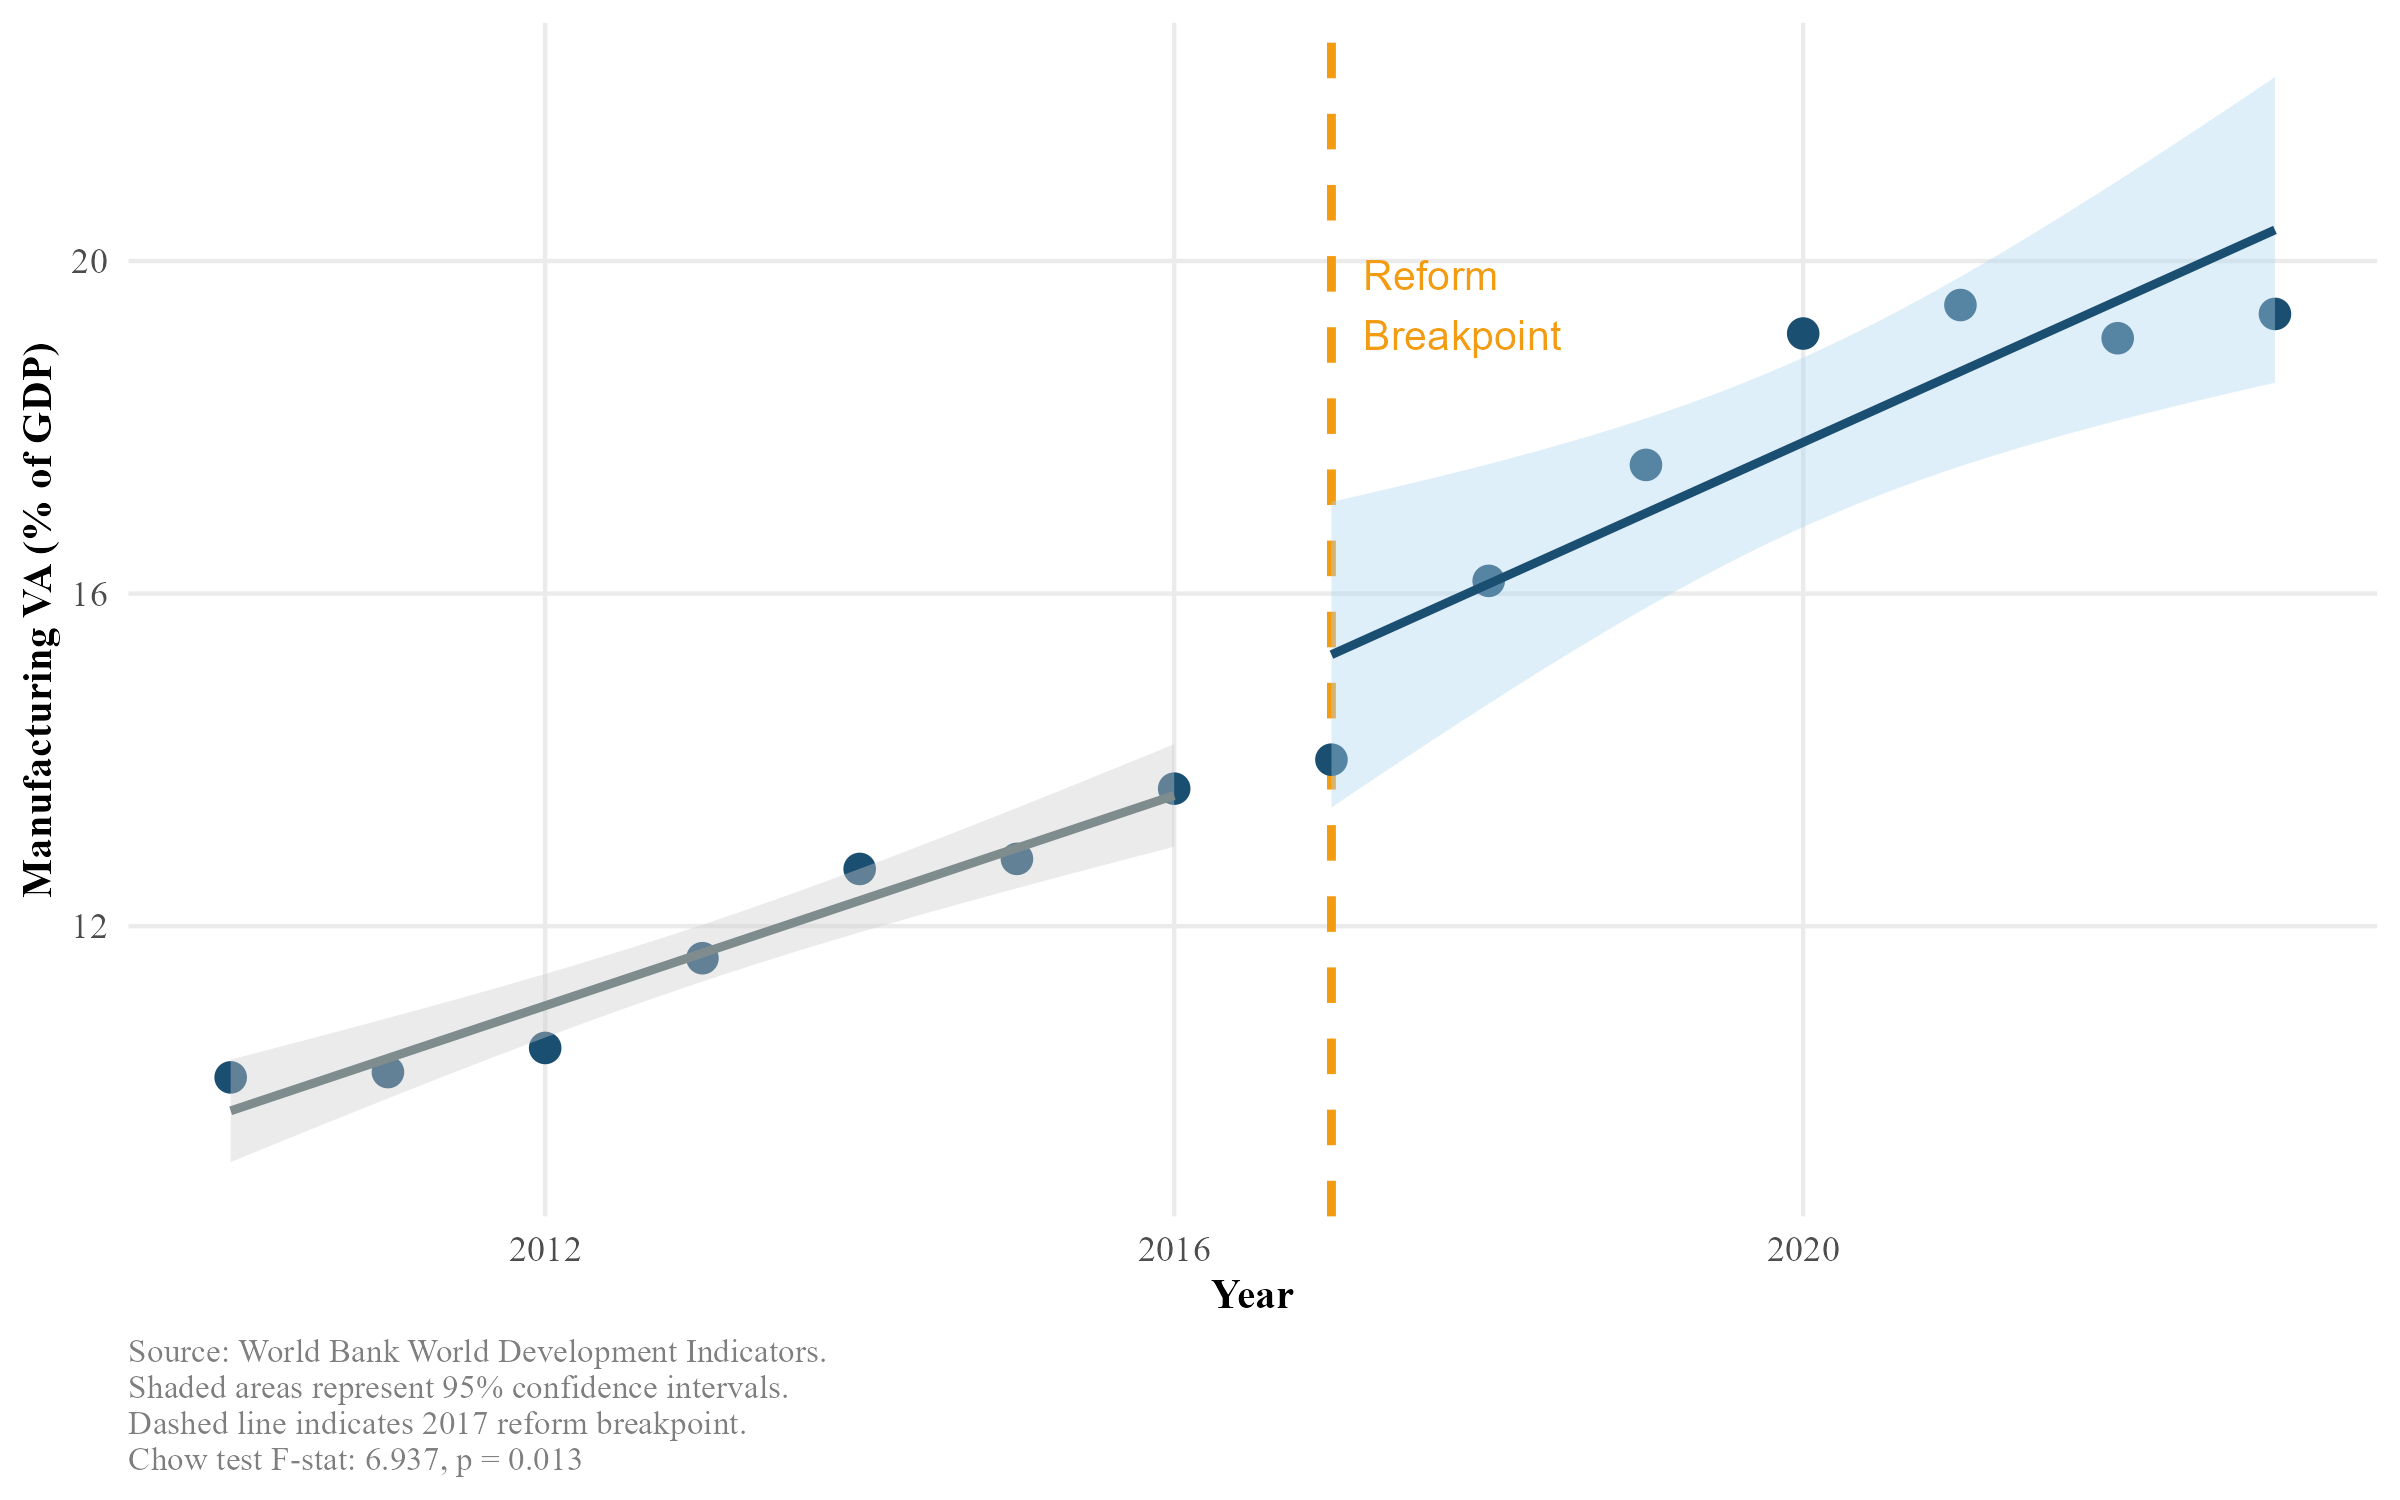
\includegraphics[width=0.85\textwidth]{figures/fig1_structural_break.png}
  \caption{Manufacturing Value Added in Uzbekistan: Structural Break at the 2017 Reform Breakpoint. The dashed vertical line marks 2017. Shaded bands represent 95\% confidence intervals for pre- and post-reform linear trends. Source: World Bank WDI.}
  \label{fig:structural_break}
\end{figure}

The Chow test confirms this visual impression. The F-statistic of 6.937 (p = 0.013) decisively rejects the null hypothesis of parameter stability at the 5\% significance level (Table \ref{tab:chow}). This constitutes robust evidence that 2017 marked a structural break in the manufacturing growth regime --- not merely a cyclical fluctuation. The pre-2017 period is characterised by modest, state-managed industrial growth averaging approximately 0.4 percentage points per year. The post-2017 period exhibits a steeper trajectory approaching 1.2 percentage points annually, consistent with the opening of the economy to foreign capital and the removal of currency convertibility restrictions that had previously made Uzbekistan unattractive to export-oriented investors.

\begin{table}[H]
  \centering
  \caption{Chow Structural Break Test Results, Manufacturing VA (\% GDP), Uzbekistan}
  \label{tab:chow}
  \begin{tabular}{lccc}
    \toprule
    Test & Breakpoint & F-statistic & p-value \\
    \midrule
    Chow test & 2017 & 6.937 & 0.013 \\
    \bottomrule
  \end{tabular}
  \\
  \small Source: Author calculations. World Bank WDI data.
\end{table}

It is important to note what the Chow test does not establish. It demonstrates that a structural break occurred, not that the Mirziyoyev reforms caused it. Confounding factors --- including the global commodity cycle, Russia's post-2014 economic difficulties reducing remittance inflows and prompting labour market restructuring in Uzbekistan, and the broader rise of Central Asia as a geopolitical pivot after the US withdrawal from Afghanistan --- all coincided with the 2017 reform period. The regression analysis in Section 8 attempts to partial out some of these confounds.


% ═══════════════════════════════════════════════════════════════════════════════
\subsection{Revealed Comparative Advantage: Export Sophistication and Its Limits}
% ═══════════════════════════════════════════════════════════════════════════════

\subsection{Overall RCA Structure}

Figure \ref{fig:rca_heatmap} presents Uzbekistan's top export sections by RCA index for selected years between 2015 and 2023. The dominant picture is one of persistent comparative advantage in primary and semi-processed commodities. Precious metals consistently exhibit the highest RCA values (indices of 20+), reflecting the dominant role of gold --- Uzbekistan is among the top ten gold producers globally. Arts and antiques, mineral products, chemical products (primarily fertilisers derived from natural gas), and base metals also show sustained RCA values comfortably above 1.

\begin{figure}[H]
  \centering
  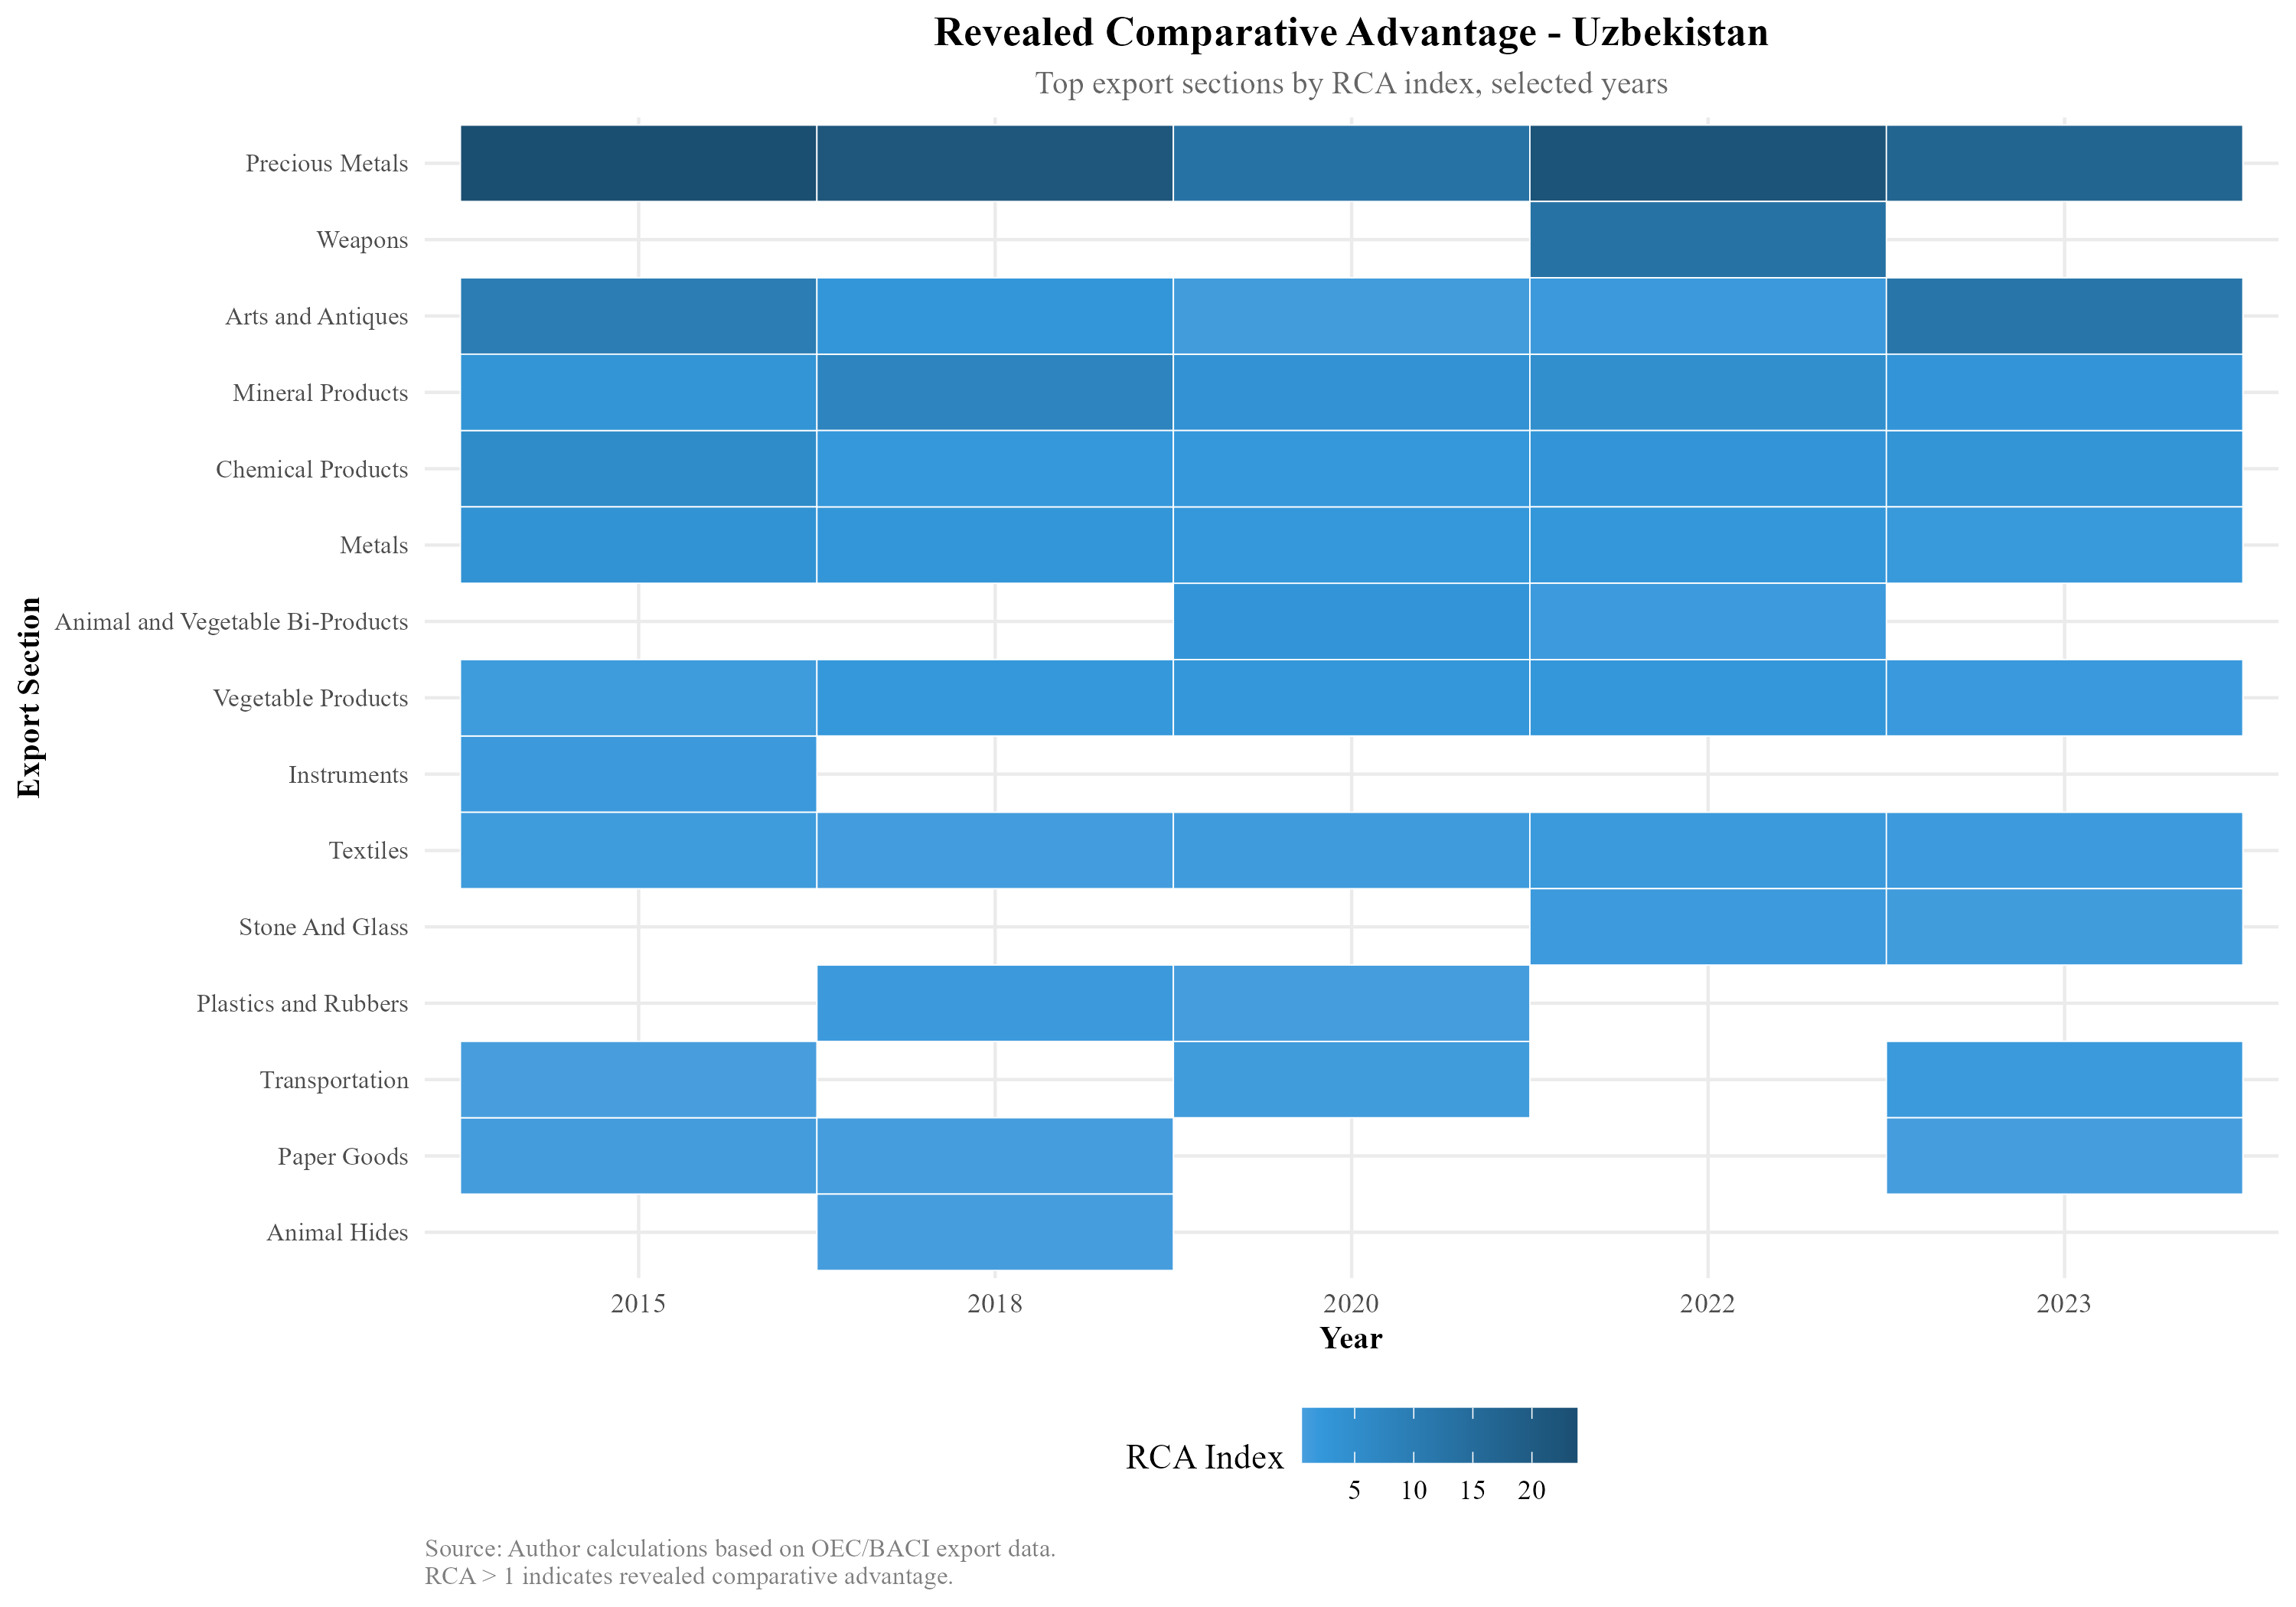
\includegraphics[width=0.90\textwidth]{figures/fig2_rca_heatmap.png}
  \caption{Revealed Comparative Advantage Heatmap, Uzbekistan: Top Export Sections by RCA Index, Selected Years 2015--2023. Darker blue indicates higher RCA. Source: Author calculations based on OEC/BACI export data.}
  \label{fig:rca_heatmap}
\end{figure}

\subsection{Manufacturing-Sector RCA Dynamics}

Figure \ref{fig:rca_manufacturing} disaggregates RCA trends for the five manufacturing-adjacent sectors most relevant to potential GVC integration: instruments, machines, metals, textiles, and transportation equipment.

\begin{figure}[H]
  \centering
  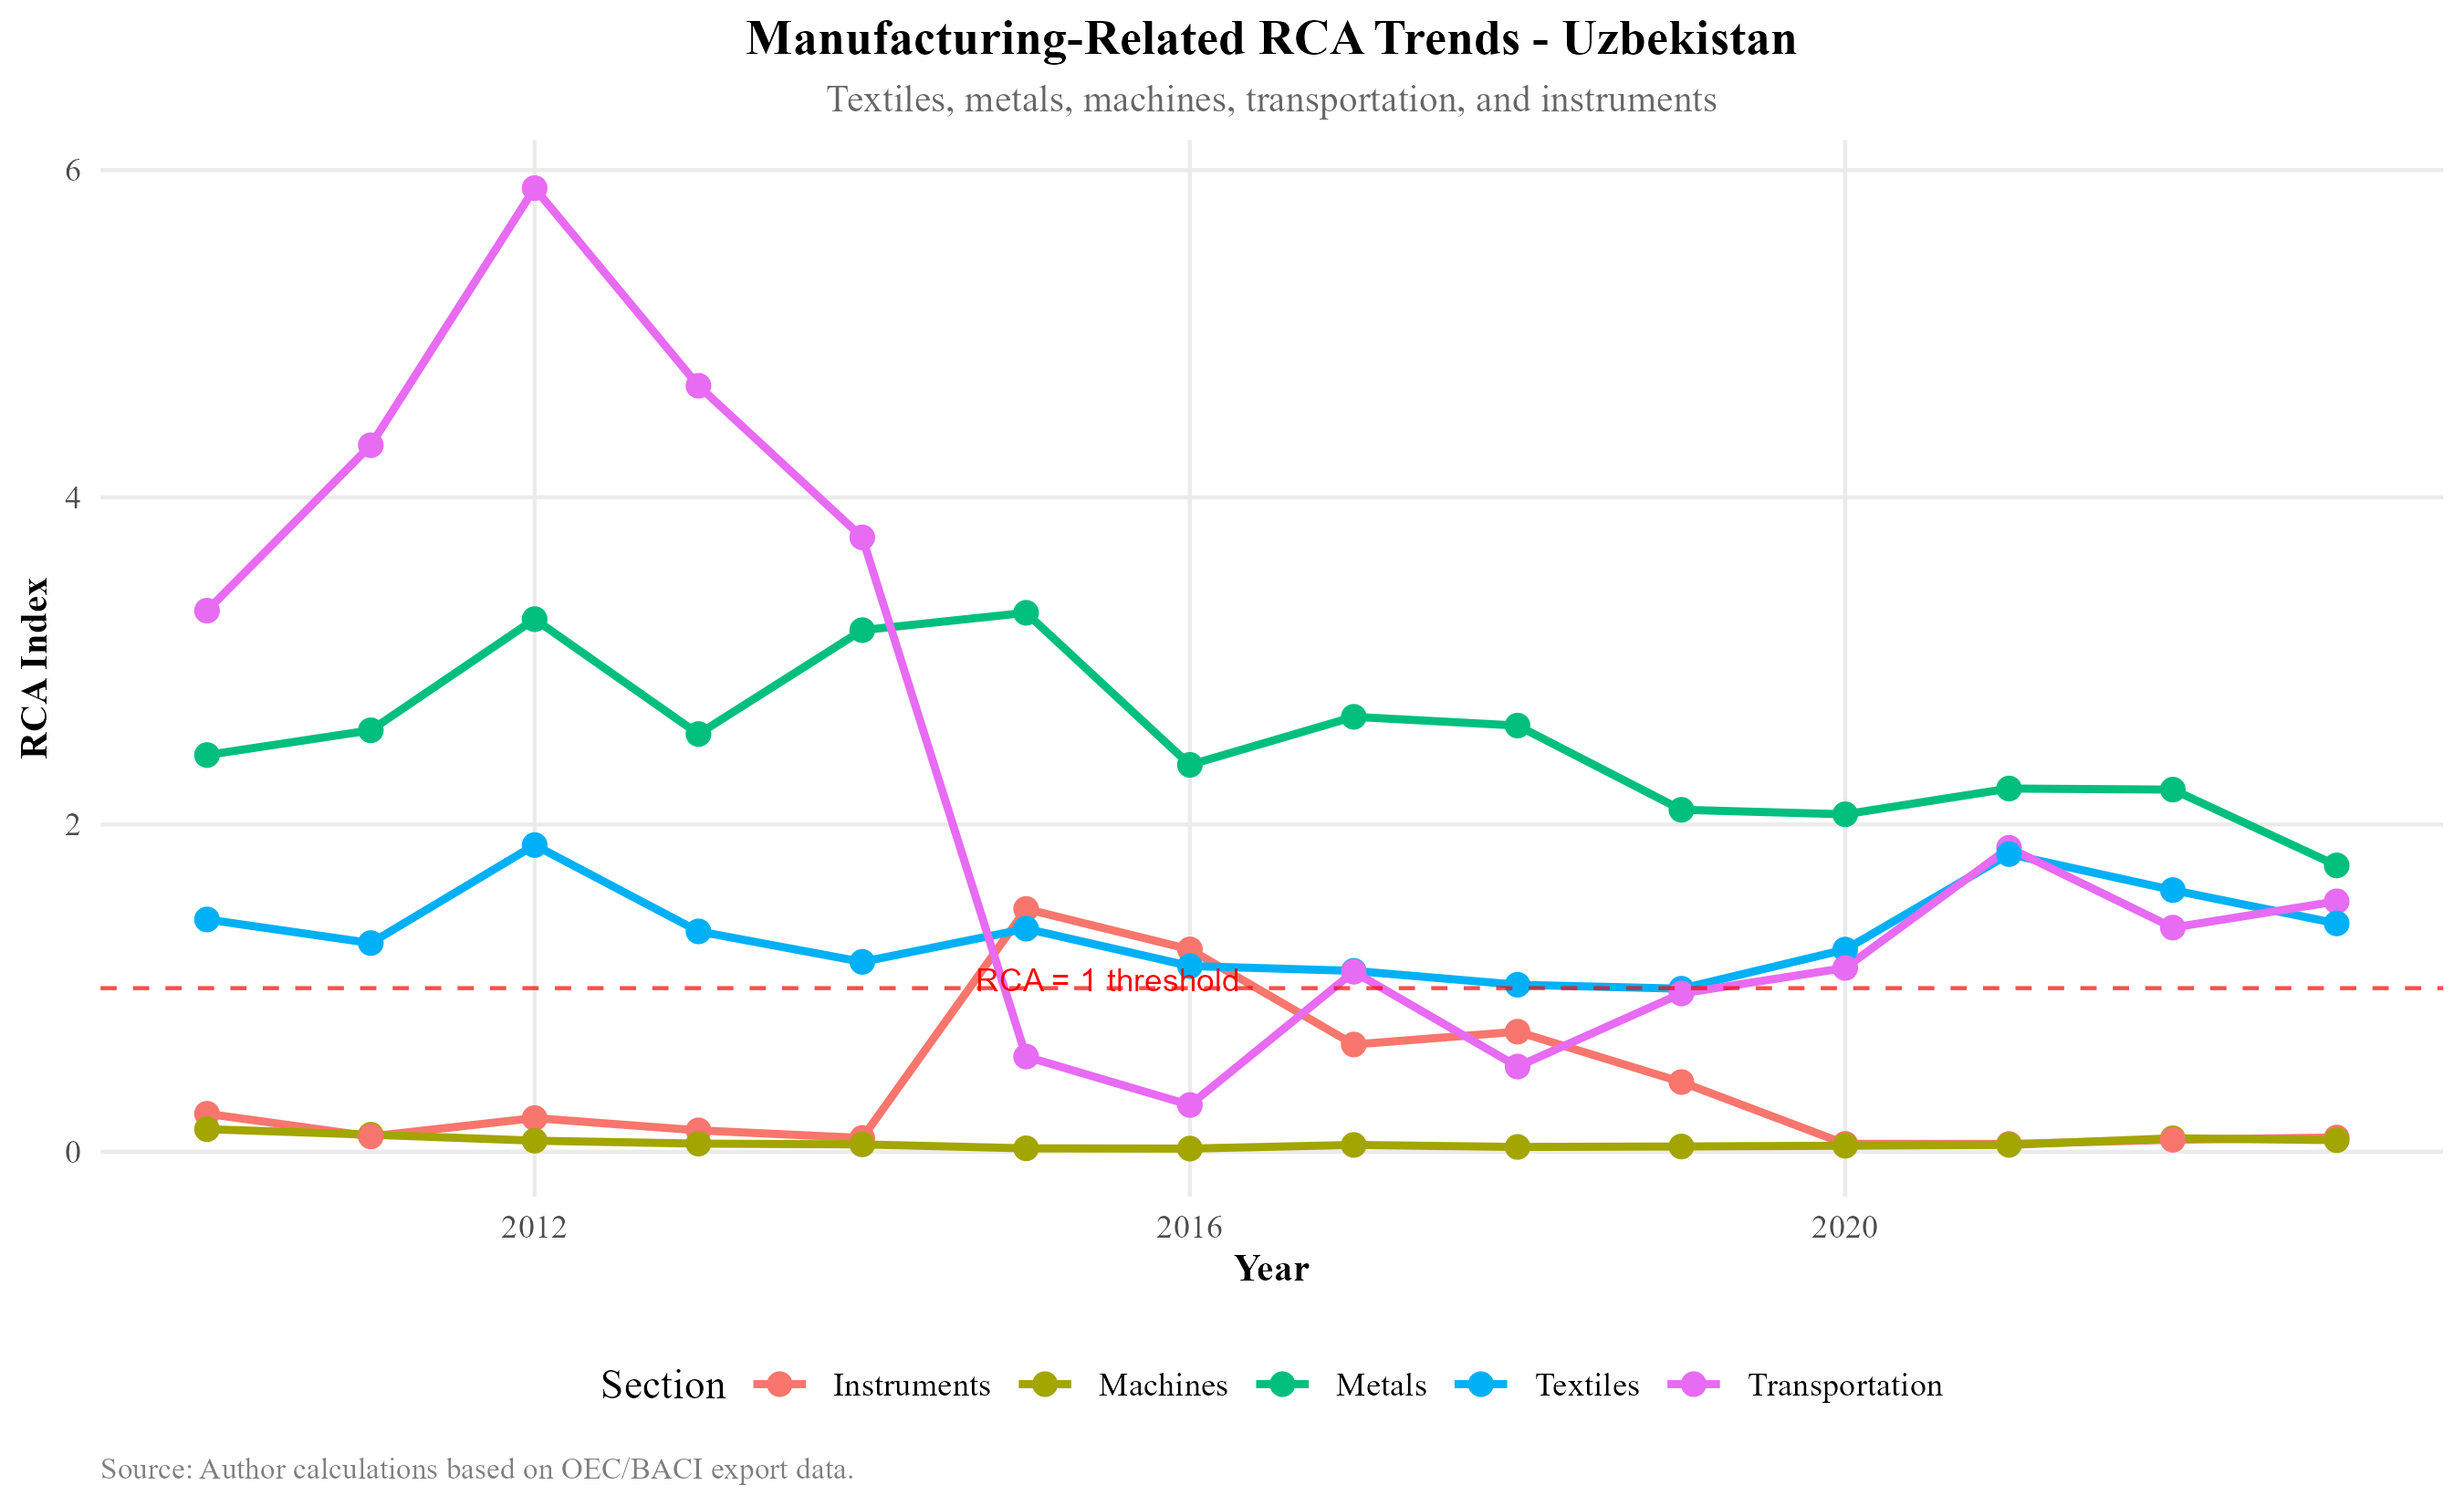
\includegraphics[width=0.85\textwidth]{figures/fig3_rca_manufacturing.png}
  \caption{Manufacturing-Related RCA Trends, Uzbekistan, 2010--2023. The horizontal dashed red line marks the RCA = 1 threshold. Source: Author calculations based on OEC/BACI export data.}
  \label{fig:rca_manufacturing}
\end{figure}

Several patterns are noteworthy. Metals maintain a consistently positive RCA above 2, driven primarily by copper and aluminium semi-manufactures that benefit from domestic mineral resource endowments. Textiles exhibited strong RCA through the early 2010s (reflecting Soviet-era cotton processing infrastructure) but have declined toward the RCA = 1 threshold, suggesting that Uzbekistan's textile comparative advantage --- once a potential anchor for GVC entry in the Bangladeshi and Vietnamese mode --- is eroding rather than deepening.

Transportation equipment showed a dramatic spike near 2012 (driven by the GM Uzbekistan joint venture, then the largest car manufacturer in the post-Soviet space) followed by collapse as the venture lost competitiveness. The subsequent rebound post-2021 coincides with the Hyundai Motor Group's involvement in the successor entity. Machines remain below 1 throughout the period, confirming that Uzbekistan has not yet developed domestic machine-building capability. Instruments declined from near-RCA-1 in the early 2010s to well below the threshold.

The manufacturing RCA profile presents a sobering picture: six years after the landmark reforms, Uzbekistan has not established new sectors of manufactured export comparative advantage. The country is growing manufacturing output --- value added is rising --- but primarily for domestic consumption and regional markets, not for sophisticated global export chains.


% ═══════════════════════════════════════════════════════════════════════════════
\subsection{Northeast Asian Trade and FDI Flows}
% ═══════════════════════════════════════════════════════════════════════════════

\subsection{Bilateral Trade Dynamics}

Figure \ref{fig:bilateral_trade} presents Uzbekistan's bilateral merchandise trade with China, Japan, and South Korea from 2010 to 2023, decomposed into total trade flows (Panel A) and trade balances (Panel B).

\begin{figure}[H]
  \centering
  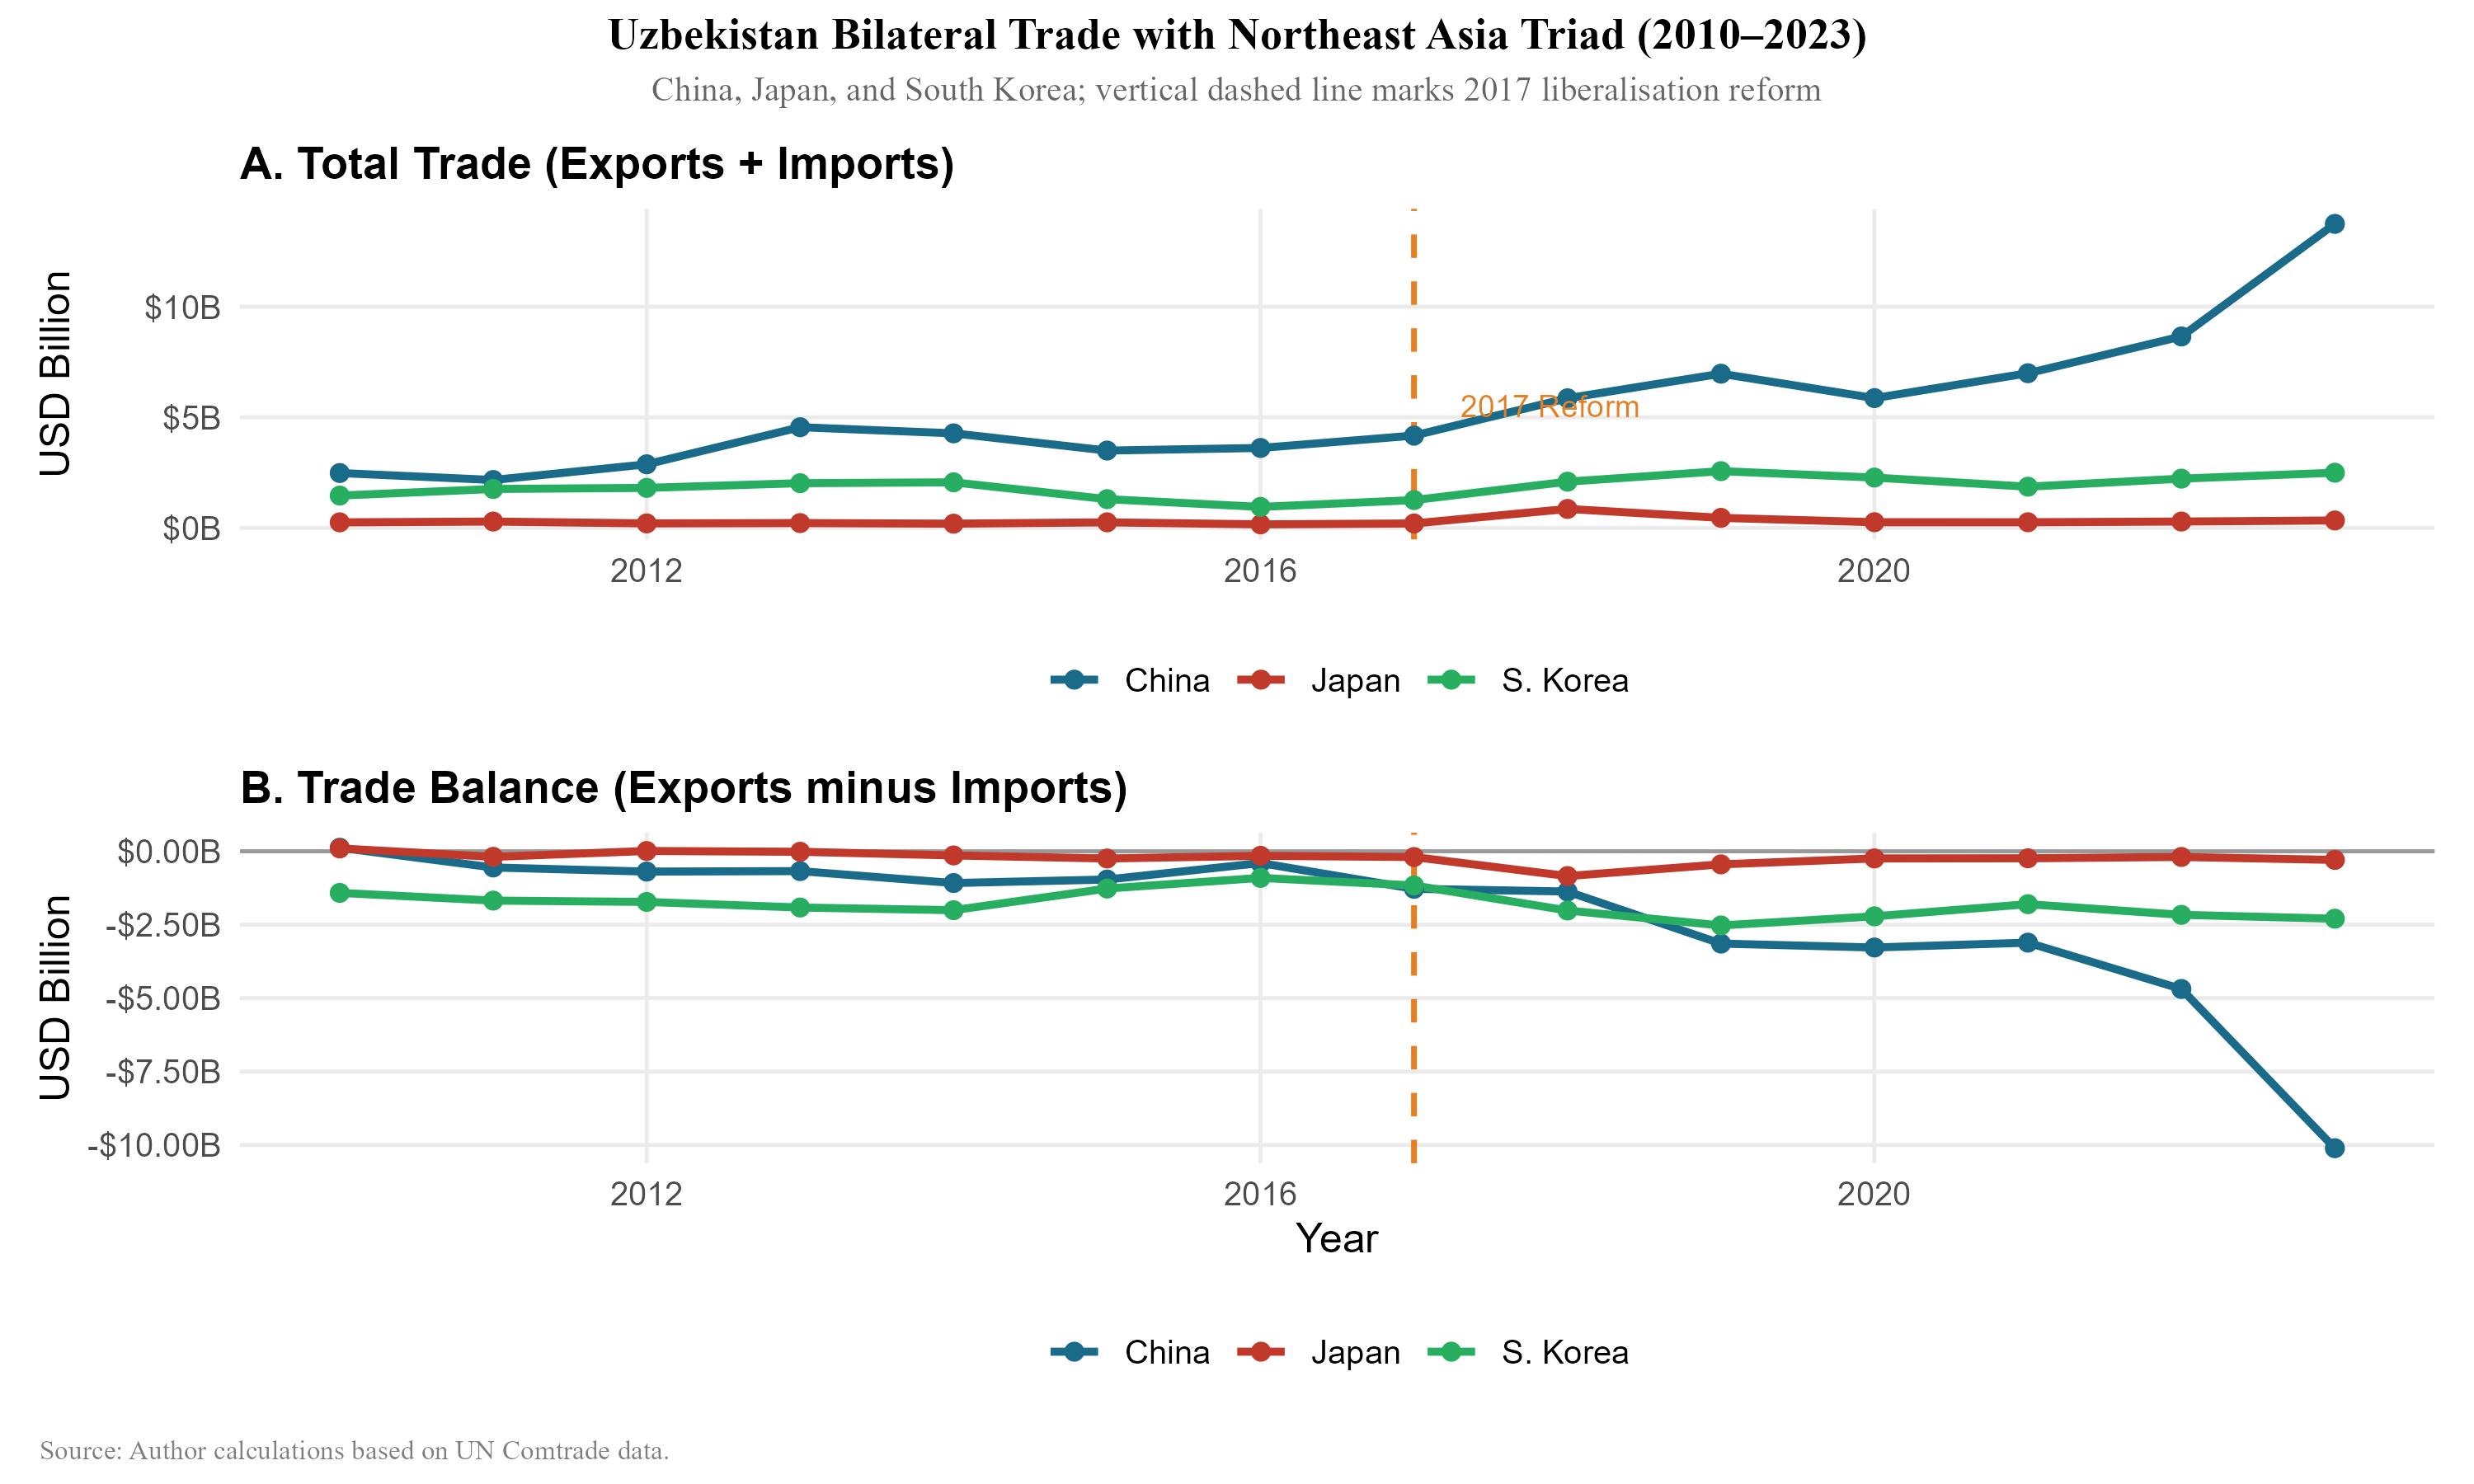
\includegraphics[width=0.90\textwidth]{figures/fig7_bilateral_trade.png}
  \caption{Uzbekistan Bilateral Trade with China, Japan, and South Korea, 2010--2023. Vertical dashed line marks the 2017 reform break. Source: OEC/BACI public API.}
  \label{fig:bilateral_trade}
\end{figure}

The China relationship dominates in both scale and growth rate. Total bilateral trade with China surged from approximately \$4 billion in 2017 to over \$12 billion by 2023 --- a 280.3\% increase --- while the trade balance deteriorated sharply to a deficit exceeding \$10 billion by 2023 (Figure \ref{fig:bilateral_trade}). This trajectory is consistent with a pattern in which Uzbekistan is importing Chinese capital goods, machinery, and intermediate inputs at scale, while exporting primary commodities (gold, cotton, copper) to China. The growing deficit is not per se a sign of harm --- if Chinese machinery imports are being absorbed into Uzbekistan's domestic manufacturing capacity, the deficit reflects investment in productive capability. However, as the intermediate goods analysis below shows, much of the Chinese import composition represents capital goods for infrastructure projects (roads, railways, power plants) financed by Chinese loans rather than export-oriented manufacturing facilities.

Japan's bilateral trade grew 110.8\% over the same period but remains small in absolute terms (well below \$1 billion), and the trade balance is near-zero. South Korea's 163\% trade growth and persistent deficit of approximately \$2.2 billion reflects imports of South Korean industrial equipment and consumer electronics rather than GVC-linked intermediate inputs.

\subsection{Intermediate Goods Composition}

Figure \ref{fig:intermediate_goods} reveals the most analytically important finding in the trade decomposition: the intermediate goods share of Uzbekistan's imports from Japan has remained at or above 95\% throughout the entire period, rising to near 100\% by 2017. South Korea's intermediate share is similarly high at approximately 88--93\%. China's intermediate goods share, by contrast, began at approximately 70\% in 2010 and rose to ~85\% by 2023.

\begin{figure}[H]
  \centering
  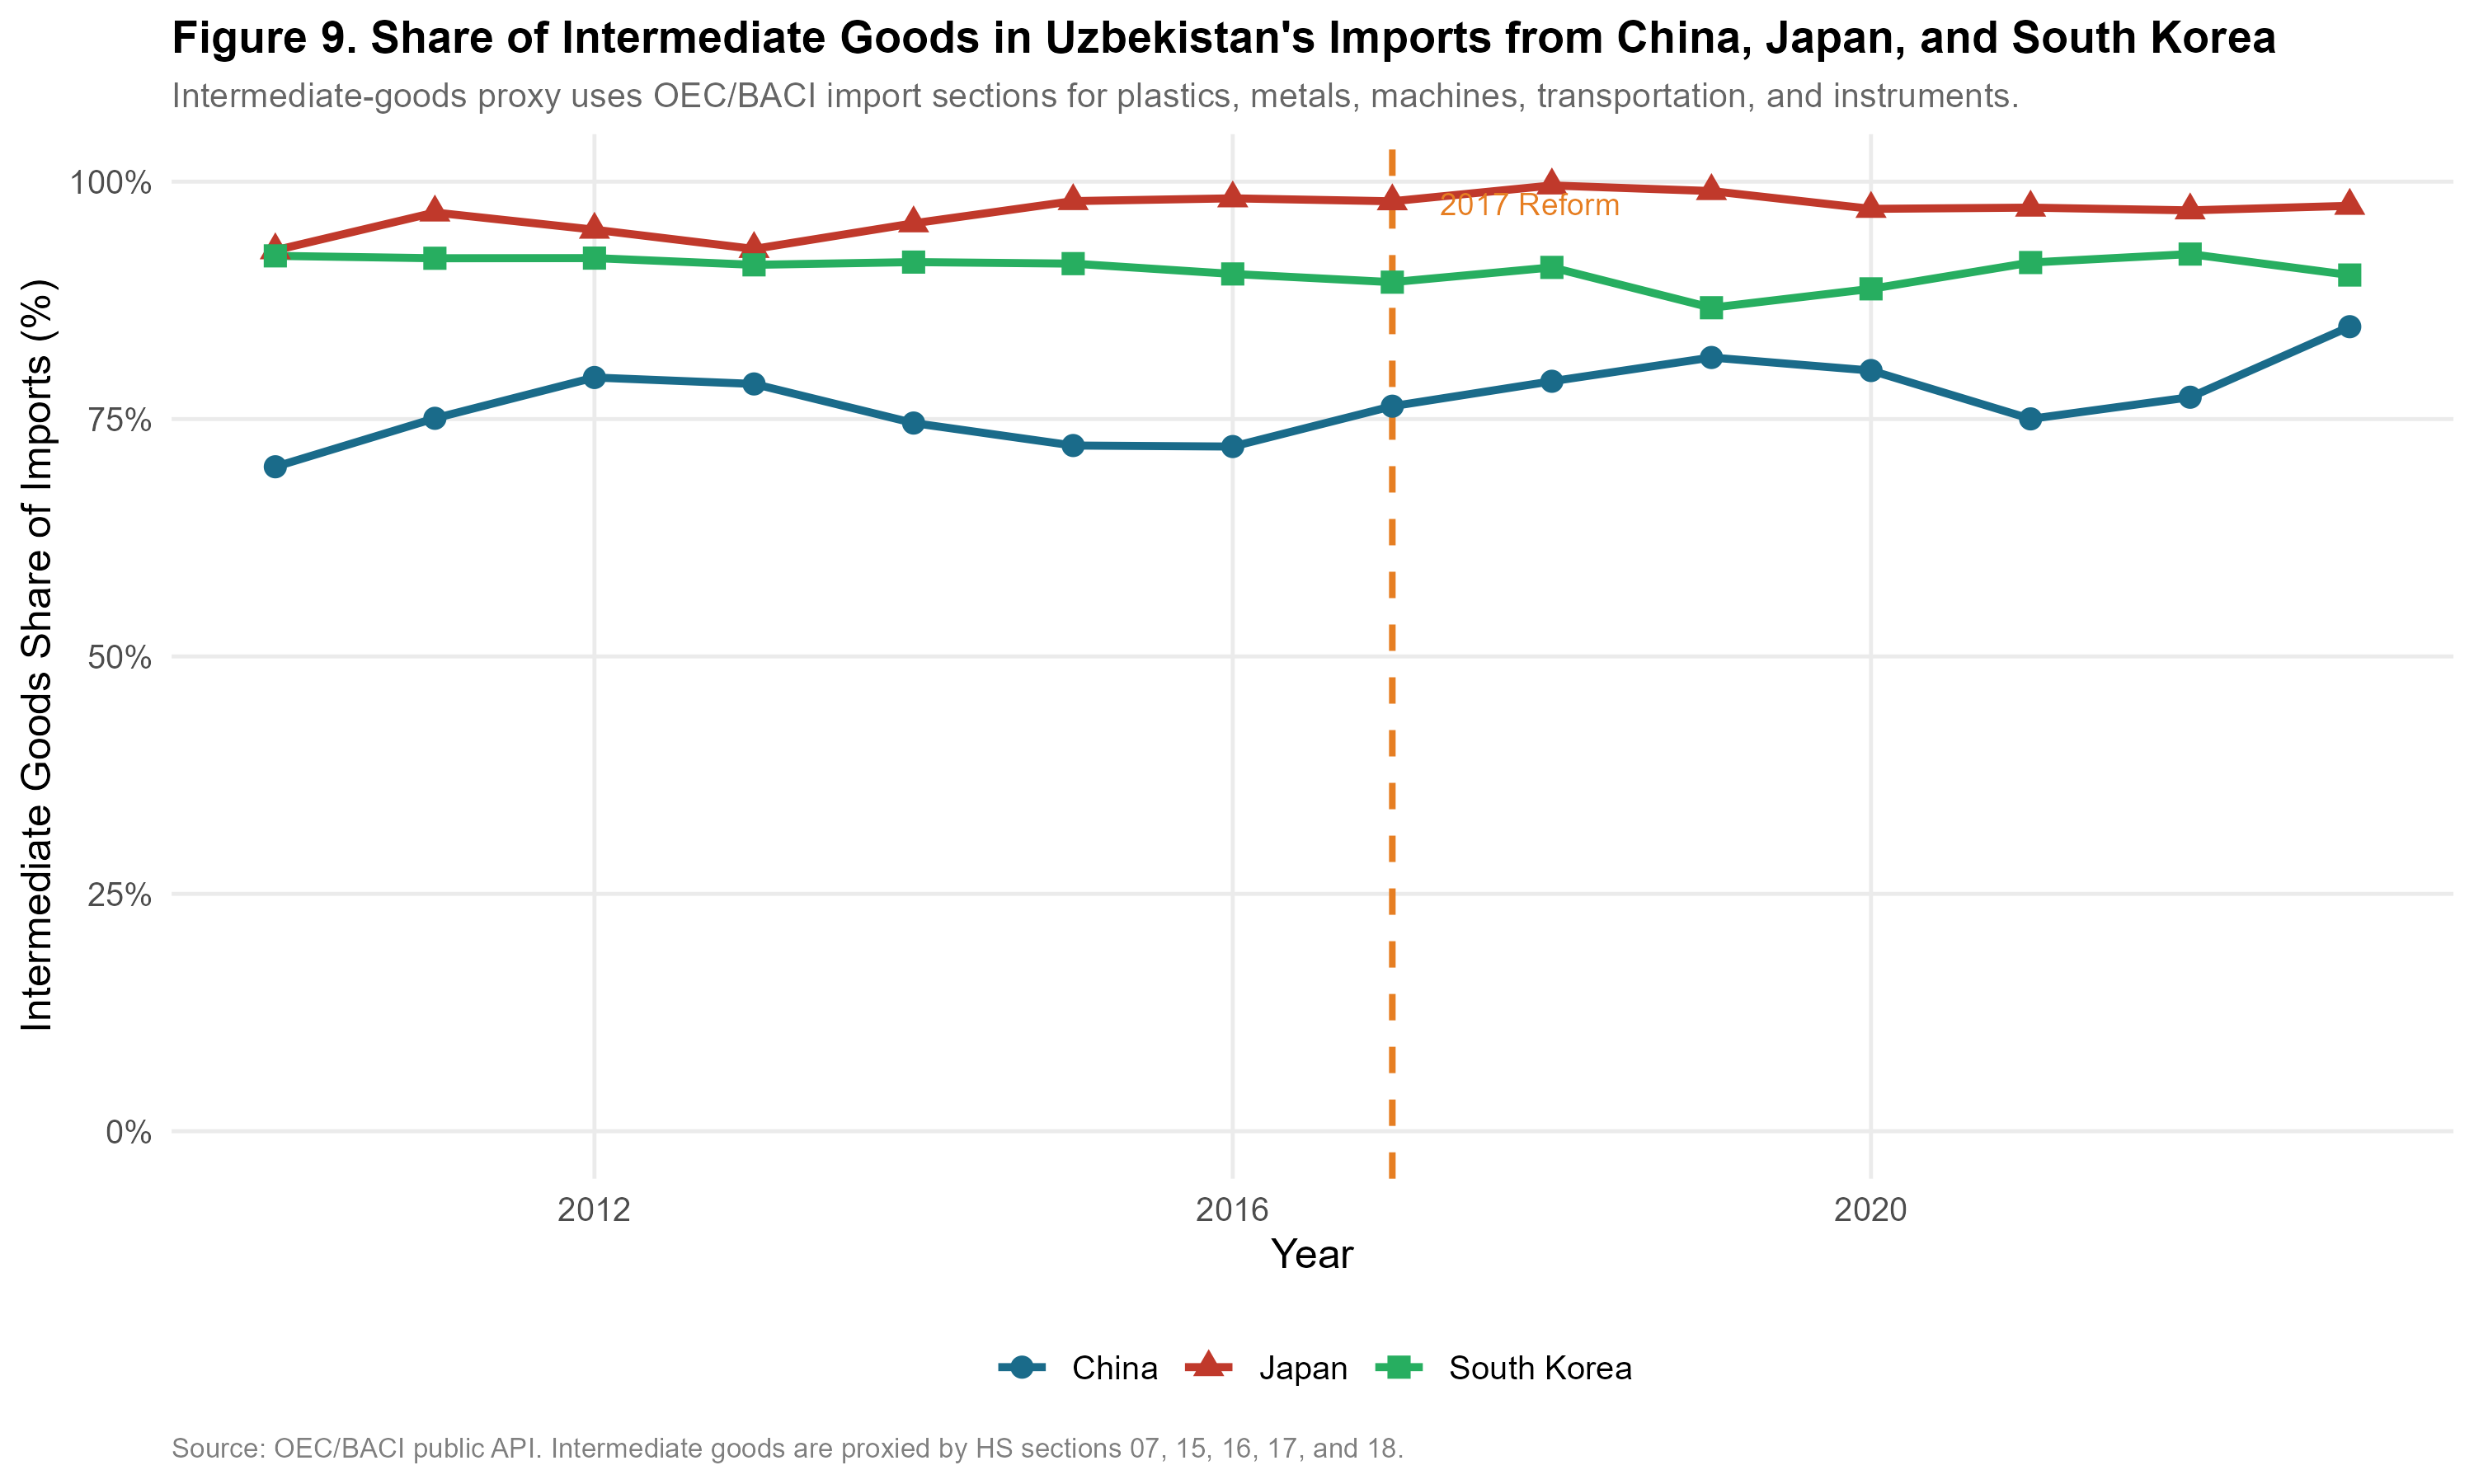
\includegraphics[width=0.85\textwidth]{figures/fig9_intermediate_goods_share.png}
  \caption{Share of Intermediate Goods in Uzbekistan's Imports from China, Japan, and South Korea. Intermediate goods proxied by HS sections 07, 15, 16, 17, and 18. Source: OEC/BACI public API.}
  \label{fig:intermediate_goods}
\end{figure}

These figures suggest that all three Northeast Asian partners are primarily supplying Uzbekistan with productive inputs rather than finished consumer goods --- a composition consistent with GVC embedding potential. However, the composition of those intermediate goods differs critically by partner. Japan's intermediate imports are concentrated in precision machinery, instruments, and transport equipment components --- technology-intensive inputs associated with higher-value manufacturing. China's intermediate imports span a wider range, from construction materials and basic metals to more sophisticated machinery, reflecting China's own broad manufacturing base and the mix of infrastructure and industrial investment in Uzbekistan.

\subsection{FDI Origin Structure}

Figure \ref{fig:fdi_origin} presents the most recent official decomposition of foreign investment and loans in fixed capital, sourced from the National Statistics Committee of Uzbekistan (2024).

\begin{figure}[H]
  \centering
  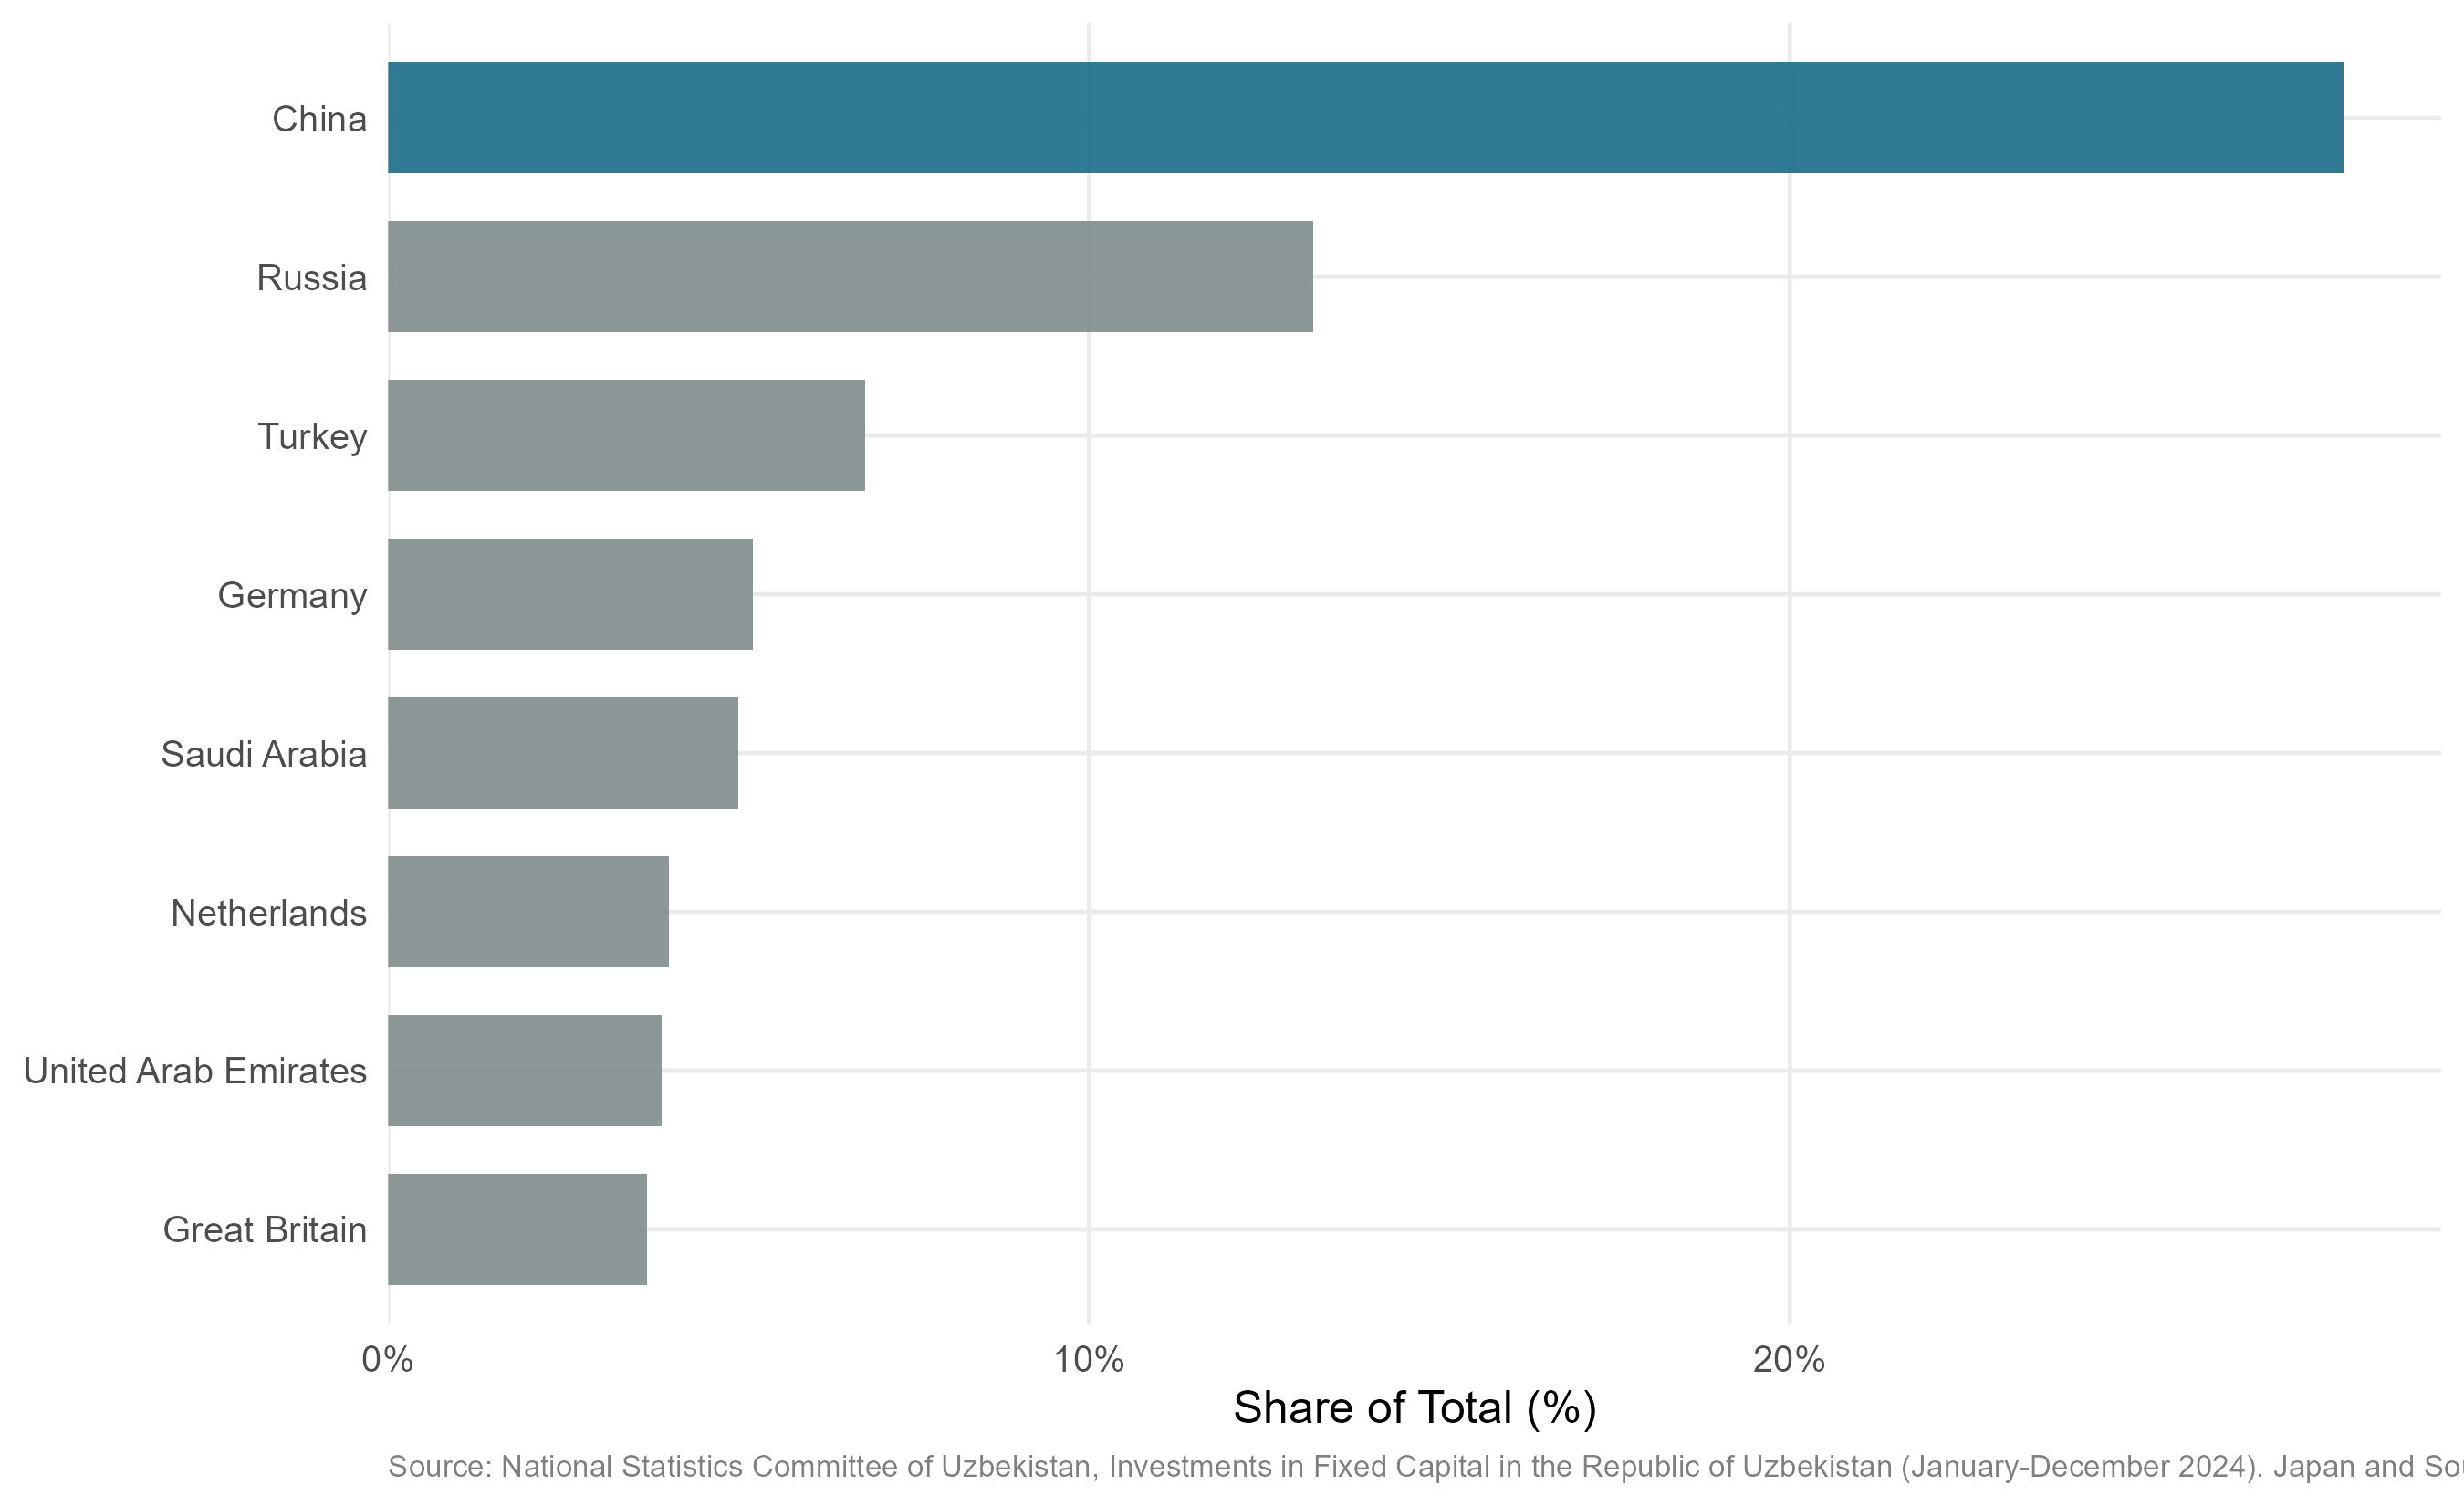
\includegraphics[width=0.85\textwidth]{figures/fig8_fdi_by_origin.png}
  \caption{Top Investor-Country Shares in Uzbekistan's Foreign Investment and Loans, 2024. Source: National Statistics Committee of Uzbekistan.}
  \label{fig:fdi_origin}
\end{figure}

China accounts for approximately 28\% of total foreign investment and loans --- the single largest source by a wide margin. Russia contributes approximately 12\%, Turkey approximately 8\%, Germany approximately 7\%, and Saudi Arabia approximately 6\%. Notably, Japan and South Korea do not appear among the top eight investors by share, suggesting that their trade relationship with Uzbekistan --- while growing rapidly in value --- has not yet translated into proportionate FDI commitments.

This FDI origin structure has important implications for the GVC embedding hypothesis. The dominant Chinese investment position, combined with evidence from the bilateral trade data showing a rapidly widening deficit, is more consistent with a Belt and Road Initiative-style infrastructure lending model than with export-oriented manufacturing FDI of the type that drove Vietnamese industrialisation (in which Japanese, Taiwanese, and South Korean electronics manufacturers established export-platform factories). The absence of Japan and Korea from the top FDI sources is the single most important gap between Uzbekistan's current integration trajectory and the Vietnamese benchmark.


% ═══════════════════════════════════════════════════════════════════════════════
\subsection{Trade Network Analysis: Value-Chain Positioning}\label{sec:network}
% ═══════════════════════════════════════════════════════════════════════════════

This section maps Uzbekistan's position in the Northeast Asian supply chain network across four analytically distinct dimensions: (i) the directed trade network structure, (ii) intermediate goods dependence by partner, (iii) export composition and structural change since 2010, and (iv) re-export potential through Central Asian and Eurasian corridors. Data are sourced from the OEC/BACI bilateral trade API (HS 1992 classification), World Bank WDI, and proxies derived from the OECD Trade in Value Added (TiVA) framework. Intermediate goods are classified using BEC Rev.~5 categories, operationalised through HS sections 05, 06, 07, 15, 16, 17, and 18.

\subsection{Value-Chain Positioning Map}

Figure~\ref{fig:trade_network_map} presents the directed trade network in which nodes represent country-actors and weighted edges represent bilateral trade flows. Node colour indicates functional role; edge colour distinguishes intermediate imports from commodity and consumer exports; edge width is proportional to the log of trade volume. Uzbekistan is placed centrally by the layout algorithm, reflecting its structural position absorbing Northeast Asian intermediate goods while exporting primary commodities outward.

A quantitative assessment of the network metrics confirms this visual configuration. Uzbekistan exhibits a high betweenness centrality (0.26) within this sub-network, reflecting its role as a conduit linking highly-connected East Asian sources (China, Korea, Japan) to Eurasian destination markets (Russia, Kazakhstan). However, while Uzbekistan possesses high in-degree connections (absorbing intermediate goods), its out-degree flows remain skewed toward lower-value commodities rather than processed manufactures. This indicates that while the country is highly connected, it is not yet embedded in dense, reciprocal production relationships---a pattern fully consistent with the captive governance structure identified earlier.

\begin{figure}[H]
  \centering
  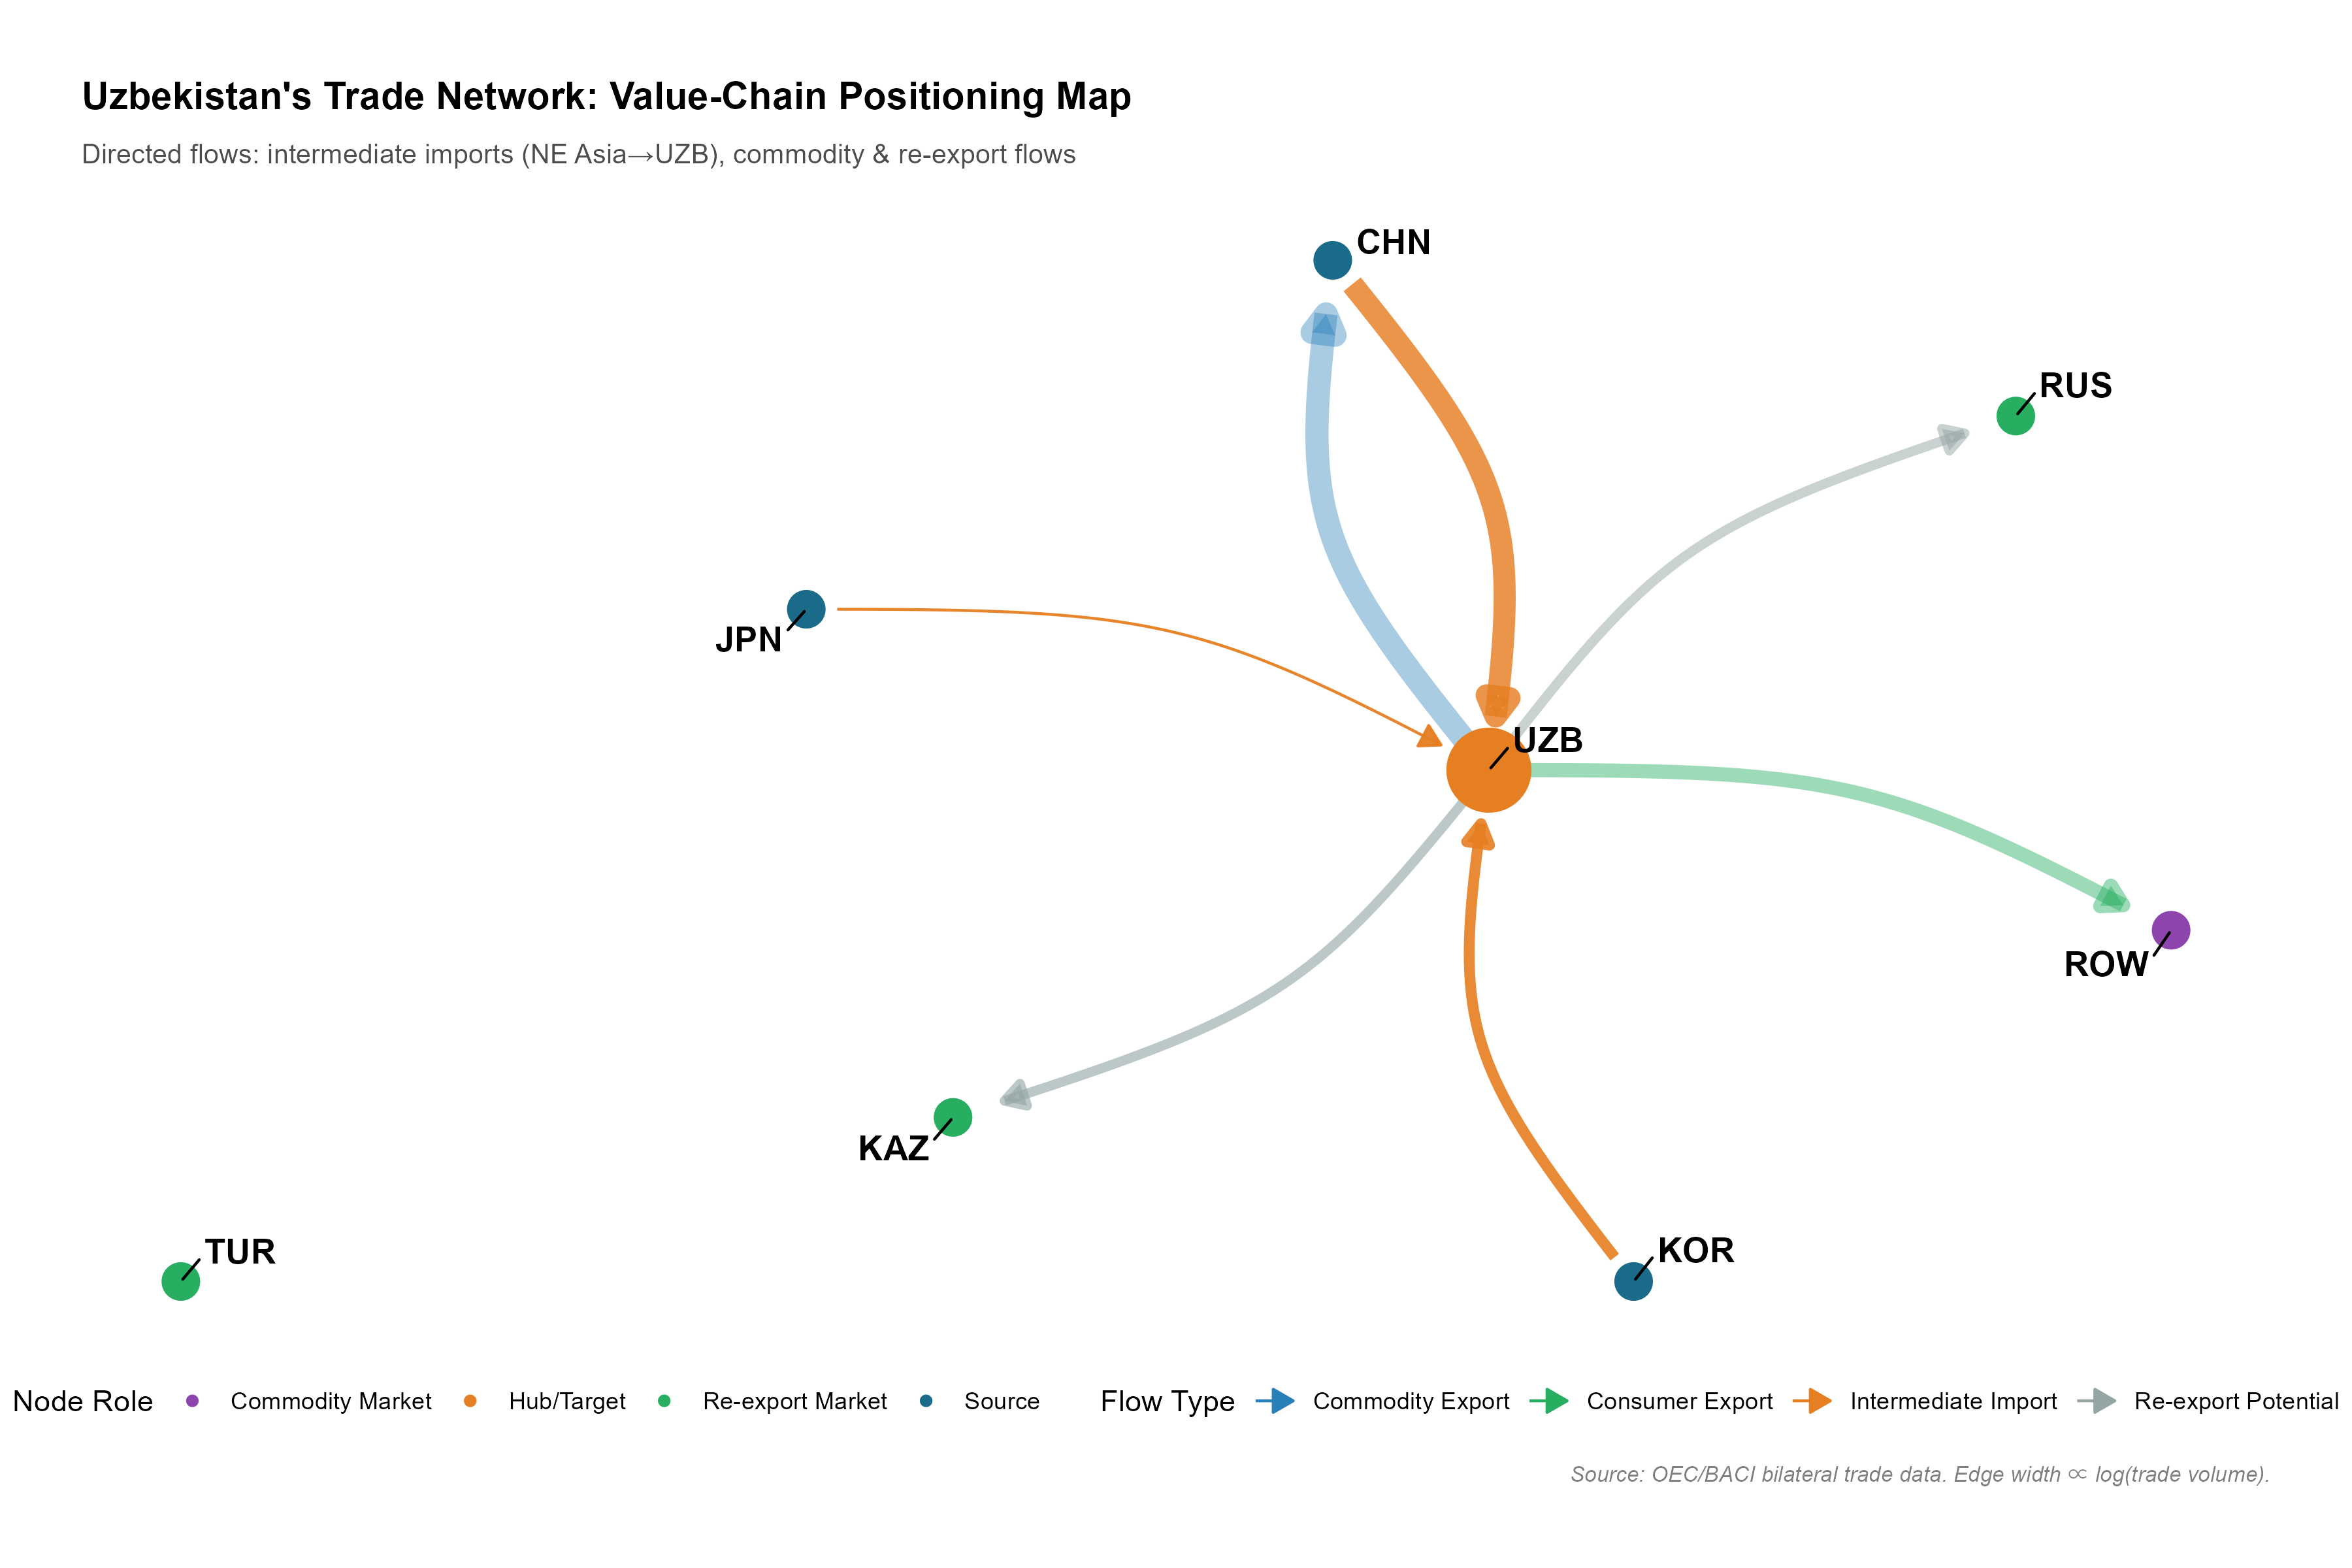
\includegraphics[width=0.92\textwidth]{figures/fig12_trade_network_map.png}
  \caption{Uzbekistan's Directed Trade Network and Value-Chain Positioning. Nodes: UZB (hub), CHN/JPN/KOR (NE Asian sources), KAZ/RUS/TUR (re-export markets), ROW (commodity destination). Edge width $\propto \log(\text{trade volume})$; opacity $\propto$ intermediate goods share. Source: Author calculations from OEC/BACI HS-section bilateral trade data.}
  \label{fig:trade_network_map}
\end{figure}

The network topology confirms the qualitative characterisation in Section~6: Uzbekistan sits structurally as a \textit{captive} node, receiving knowledge-intensive intermediate goods from all three Northeast Asian partners and exporting primary commodities outward. The graph also reveals a thin but non-zero set of edges from Uzbekistan toward Kazakhstan, Russia, and Turkey --- potential re-export corridors that could be thickened by deliberate GVC integration policy.

\subsection{Intermediate Goods Dependence by Partner}

Figure~\ref{fig:intermediate_dependence} disaggregates the intermediate goods story into two panels: the share of intermediate goods in total imports from each NE Asian partner (Panel A), and the absolute volume (Panel B).

\begin{figure}[H]
  \centering
  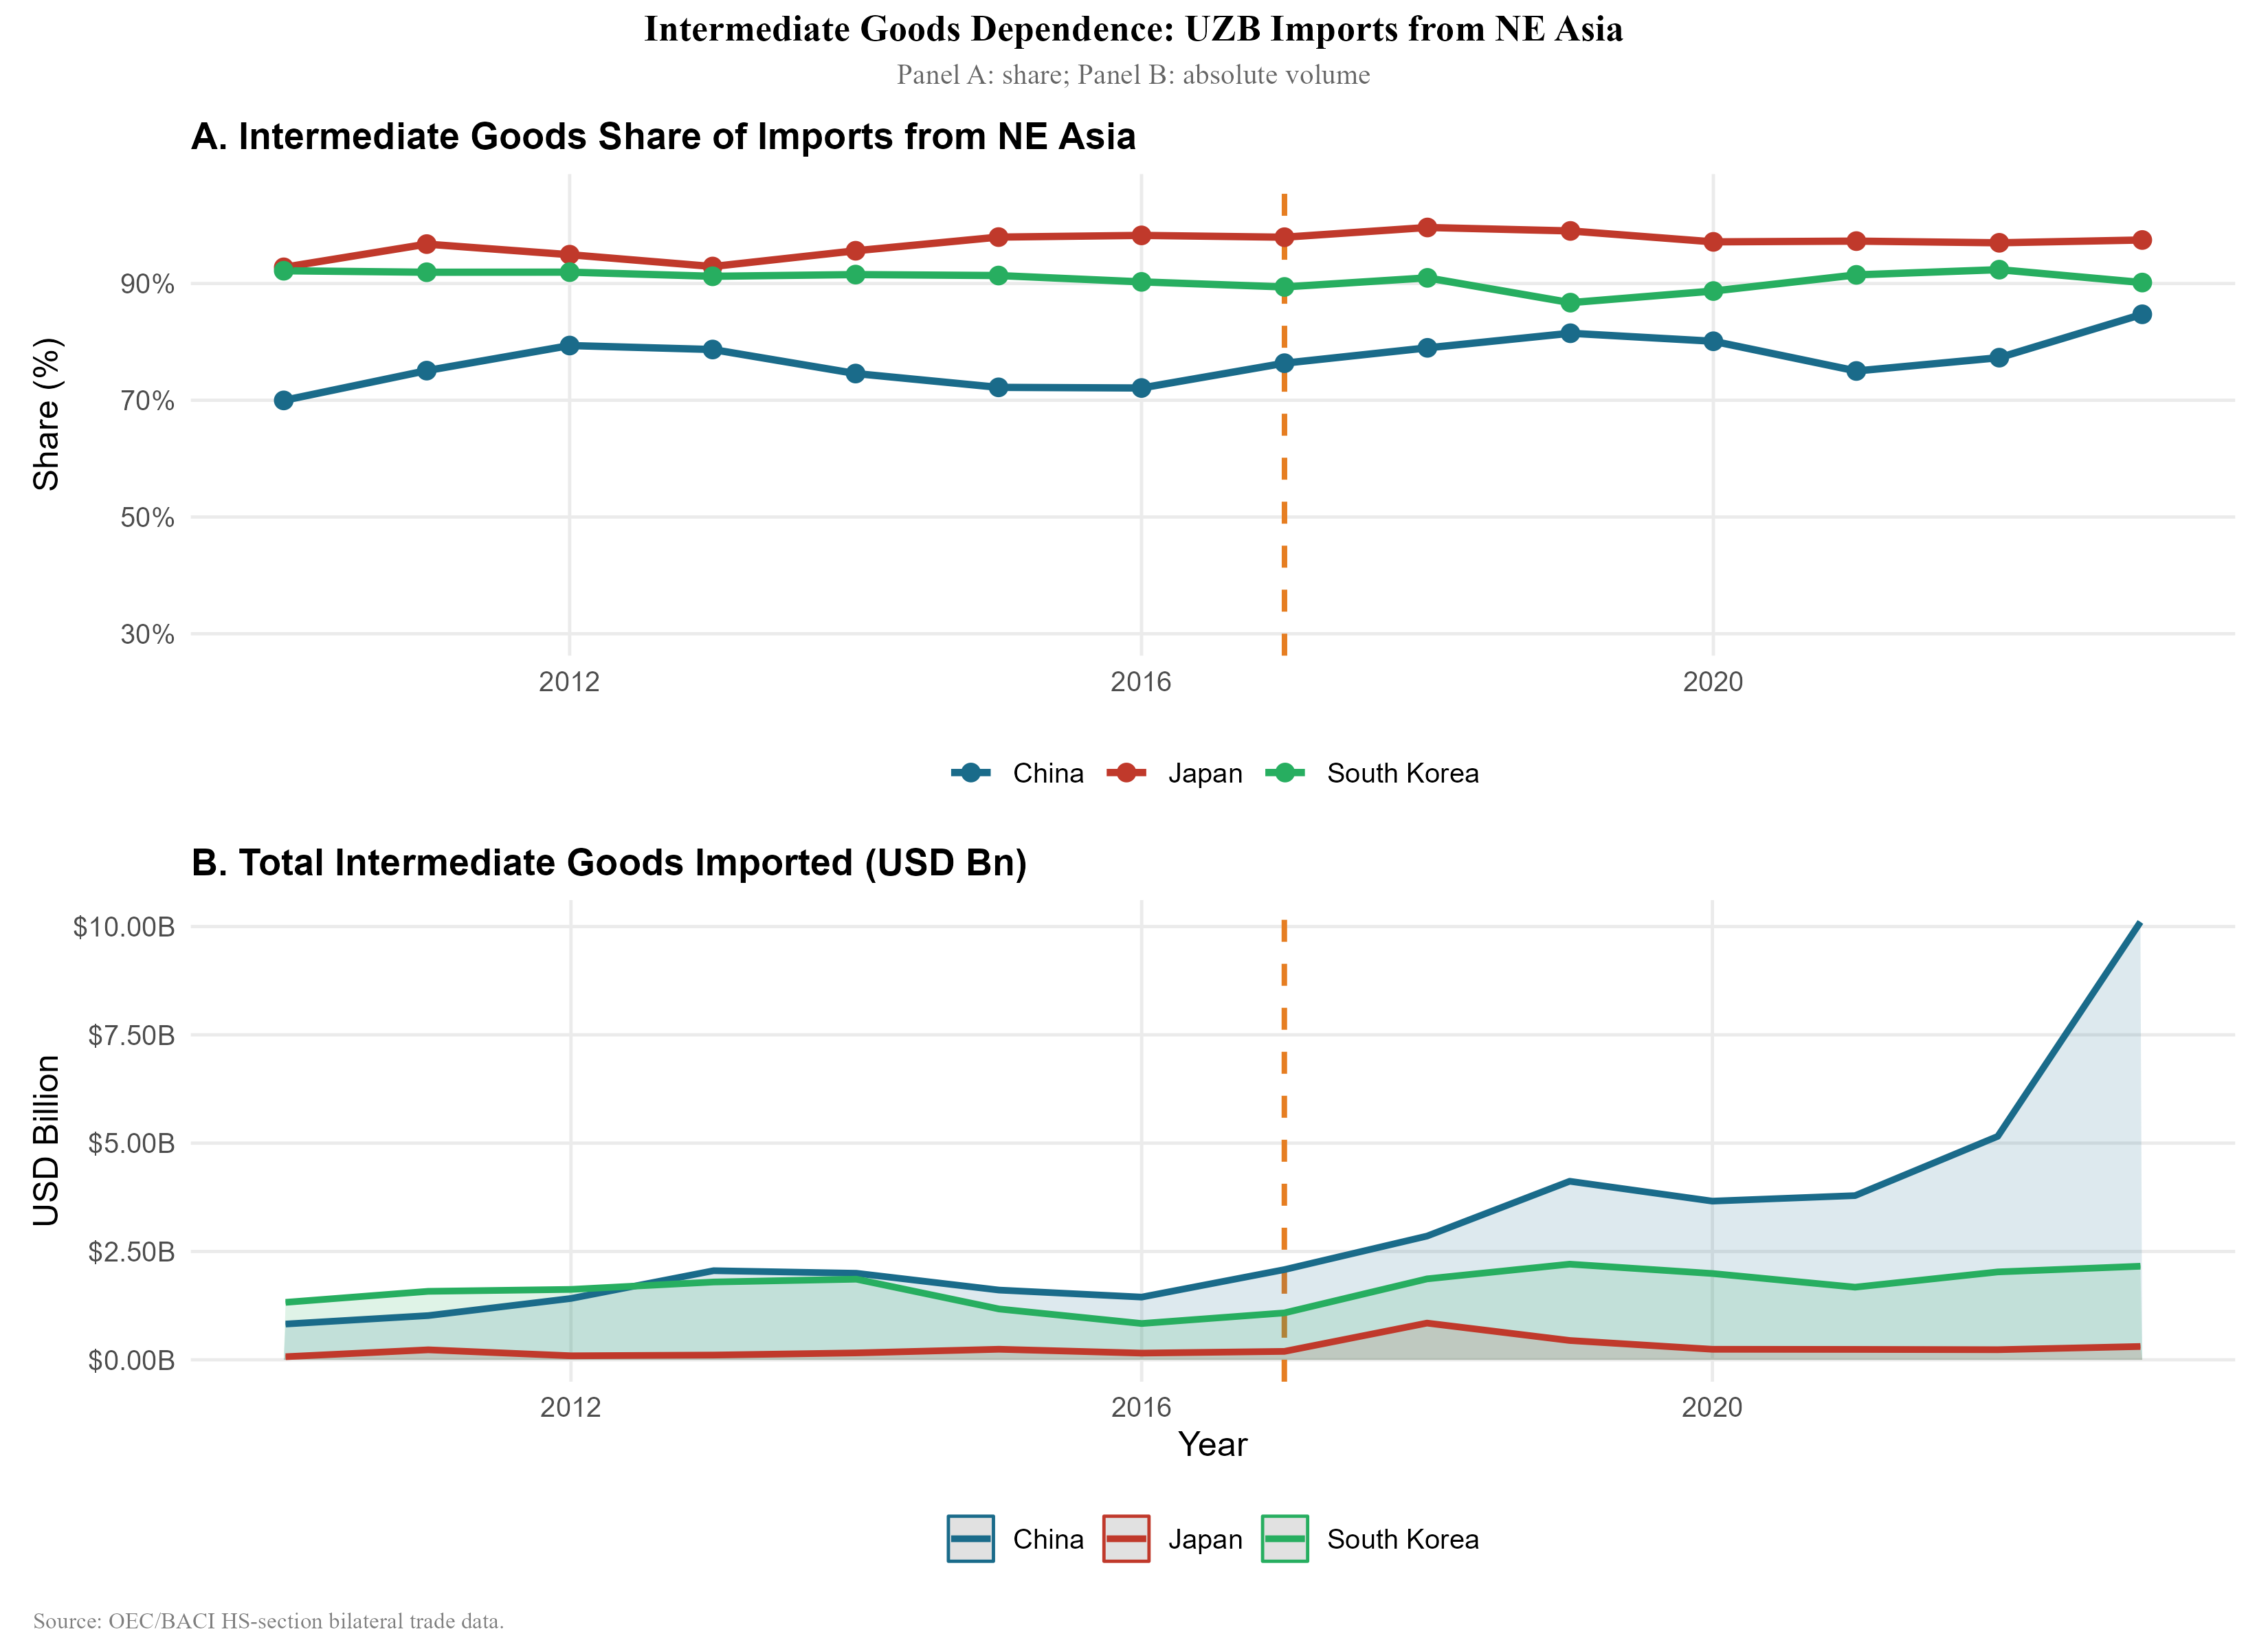
\includegraphics[width=0.90\textwidth]{figures/fig13_intermediate_dependence.png}
  \caption{Intermediate Goods Dependence: Uzbekistan's Imports from Northeast Asia, 2010--2023. Panel A: intermediate goods share (\%); Panel B: absolute volume (USD bn). BEC Rev.5 classification: HS sections 05, 06, 07, 15, 16, 17, 18. Vertical dashed line marks the 2017 reform break. Source: Author calculations from OEC/BACI bilateral trade data.}
  \label{fig:intermediate_dependence}
\end{figure}

Three findings emerge. \textbf{First}, Japan's intermediate share consistently approaches 95--100\%, confirming that Japan's bilateral relationship is almost entirely GVC-relevant, comprising precision machinery, instruments, and transport components. \textbf{Second}, South Korea's share (88--93\%) is similarly high and stable, consistent with Samsung SDI supply-chain negotiations documented in the policy literature. \textbf{Third}, China's share (70--85\%) has risen steadily since 2017, reflecting the growing share of machinery in Belt and Road-linked investment. In absolute volume (Panel B), Chinese intermediate imports dwarf Japan and Korea combined.

\subsection{Export Composition: Structural Change 2010--2023}

Figure~\ref{fig:export_composition} presents Uzbekistan's export basket by HS-level goods category in share (Panel A) and absolute volume (Panel B) over 2010--2023.

\begin{figure}[H]
  \centering
  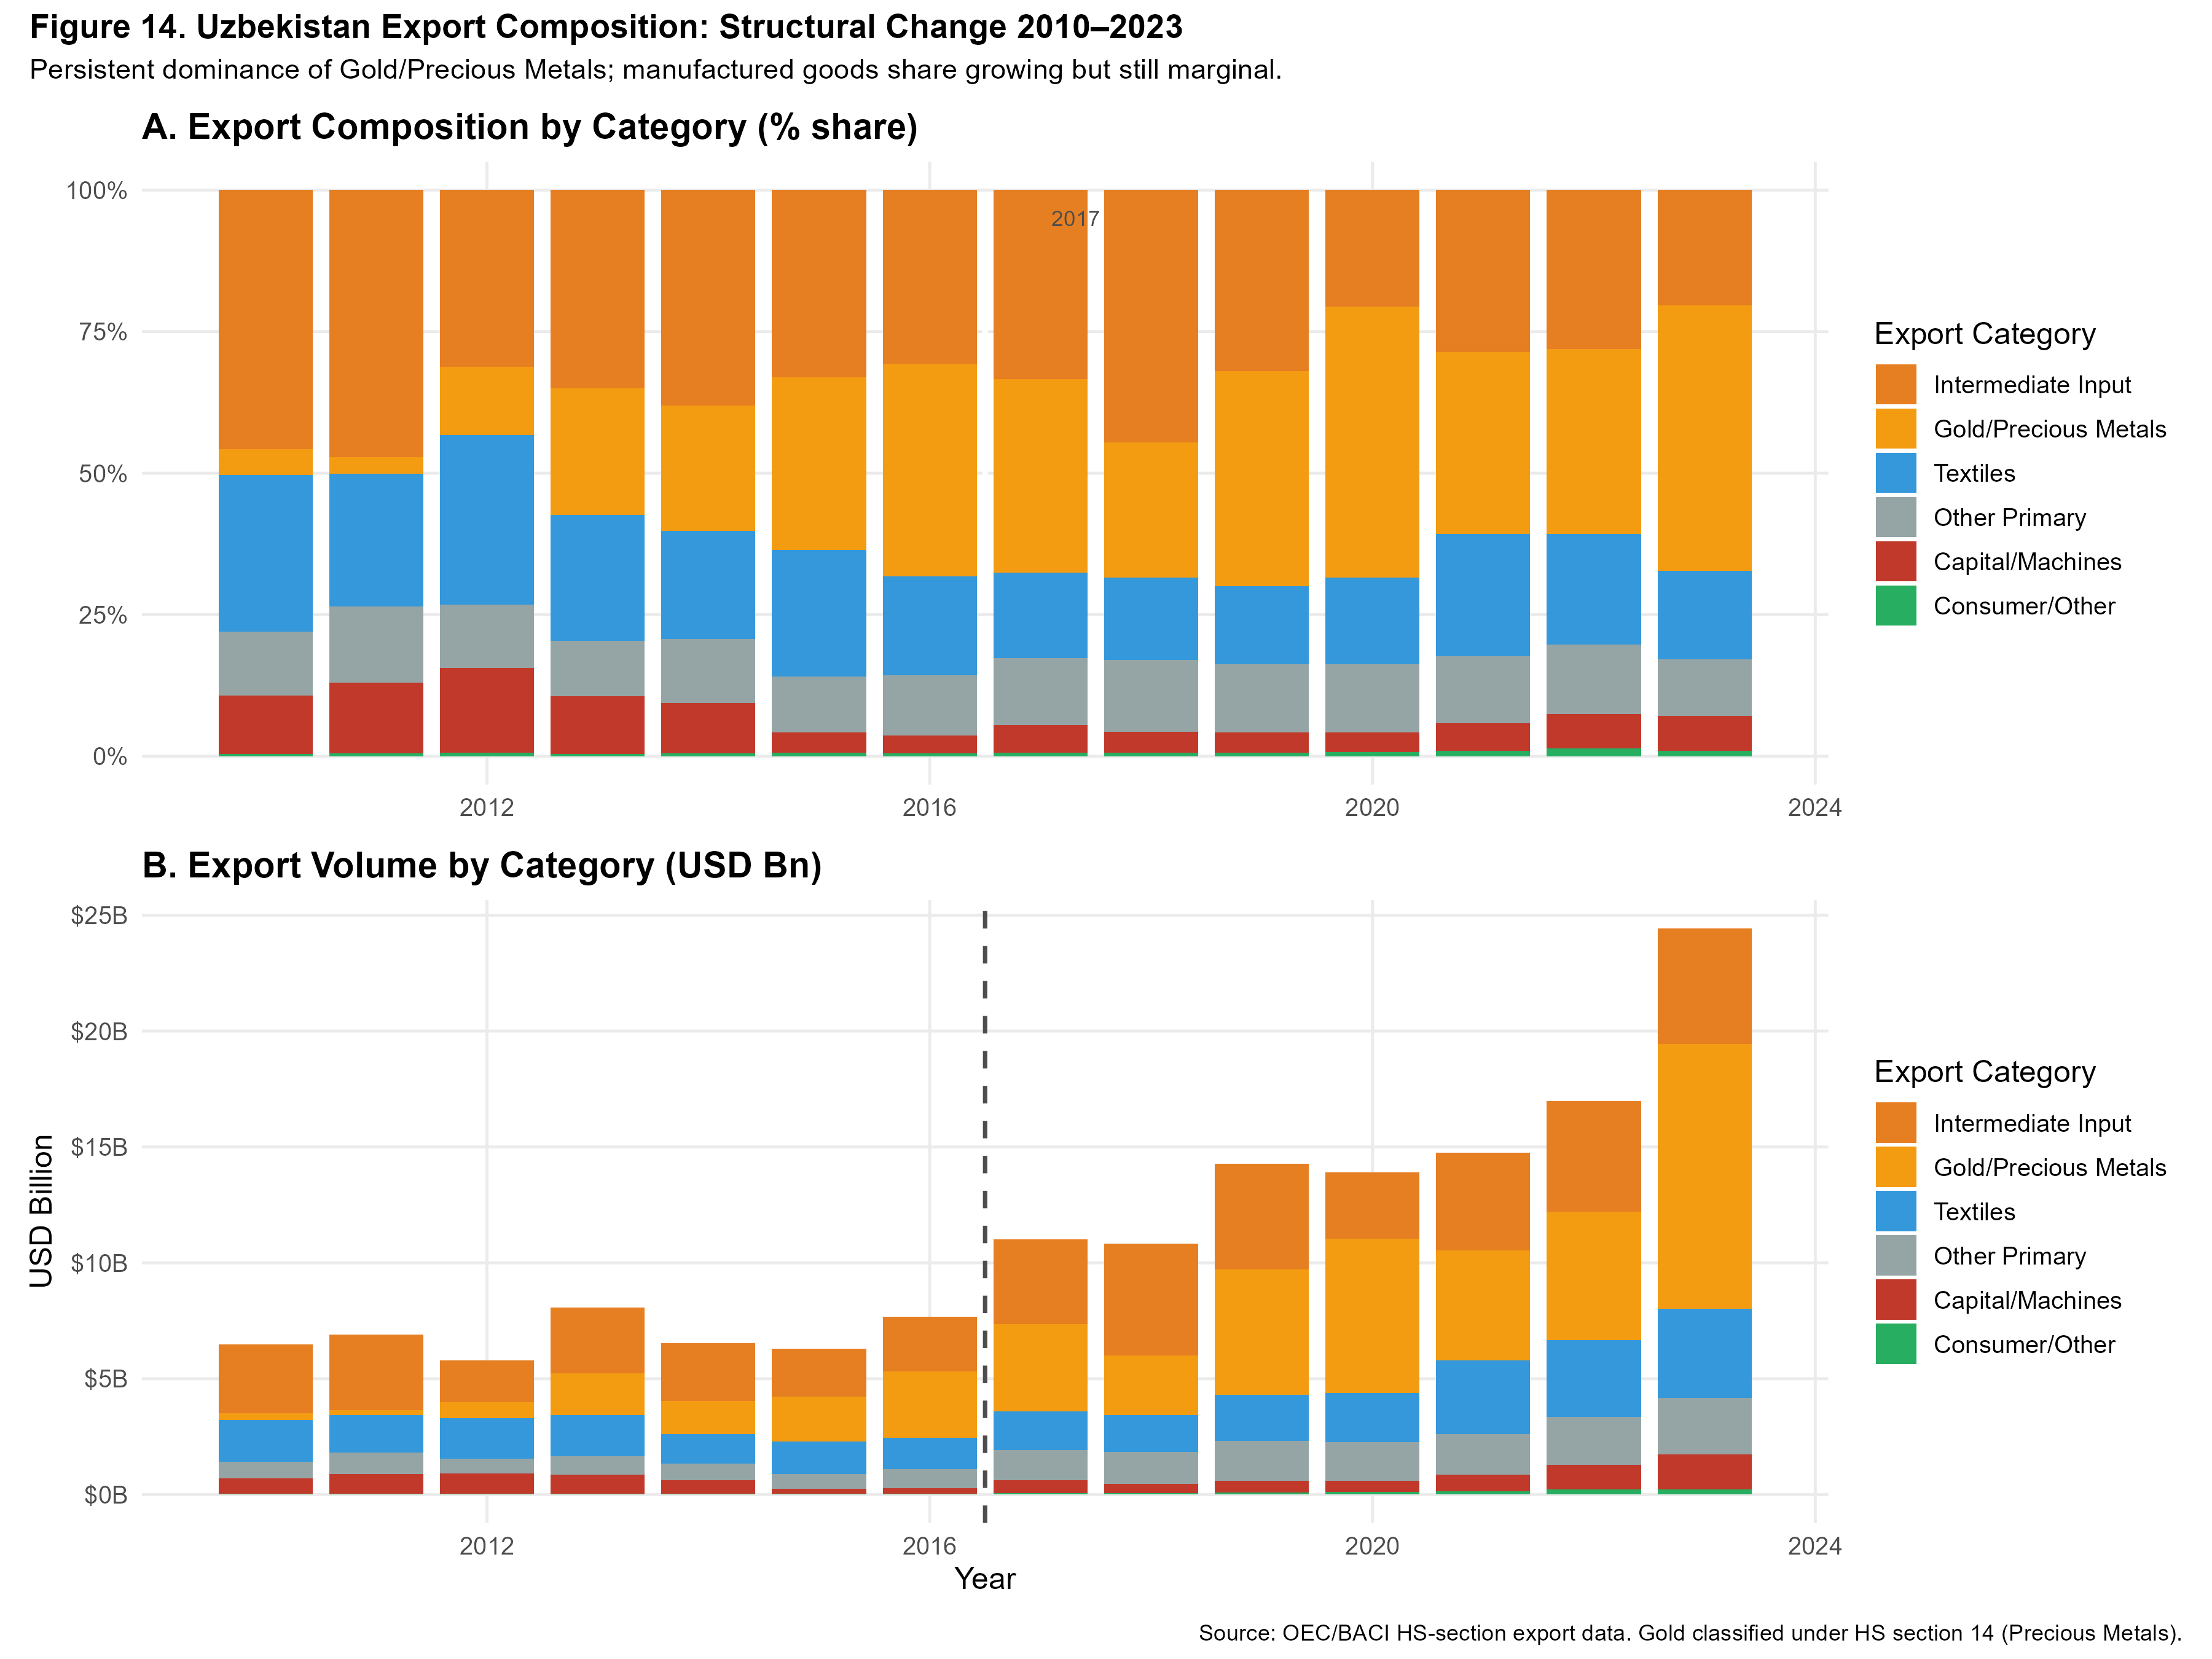
\includegraphics[width=0.92\textwidth]{figures/fig14_export_composition.png}
  \caption{Uzbekistan Export Composition by Category, 2010--2023. Panel A: category shares (\%); Panel B: absolute volumes (USD bn). Gold/Precious Metals (HS 14) dominate throughout. Vertical dashed line marks the 2017 reform. Source: Author calculations from OEC/BACI HS-section export data.}
  \label{fig:export_composition}
\end{figure}

The evidence is unambiguous: gold and precious metals (HS 14) account for 50--60\% of total export value in most post-reform years. Textiles (HS 11) represent the second-largest category at 15--20\% by 2023. Manufactured and machinery exports (HS 15--18 combined) remain below 10\% in aggregate, despite the post-reform opening. Uzbekistan is absorbing technology-intensive inputs from Northeast Asia but exporting primary commodities, with minimal value-added conversion --- the defining symptom of shallow GVC embedding.

\subsection{Re-export Potential Through Central Asian Corridors}

Figure~\ref{fig:reexport_potential} maps the re-export potential of Uzbekistan's manufactured goods flows toward Kazakhstan, Russia, Turkey, and the Rest of World.

\begin{figure}[H]
  \centering
  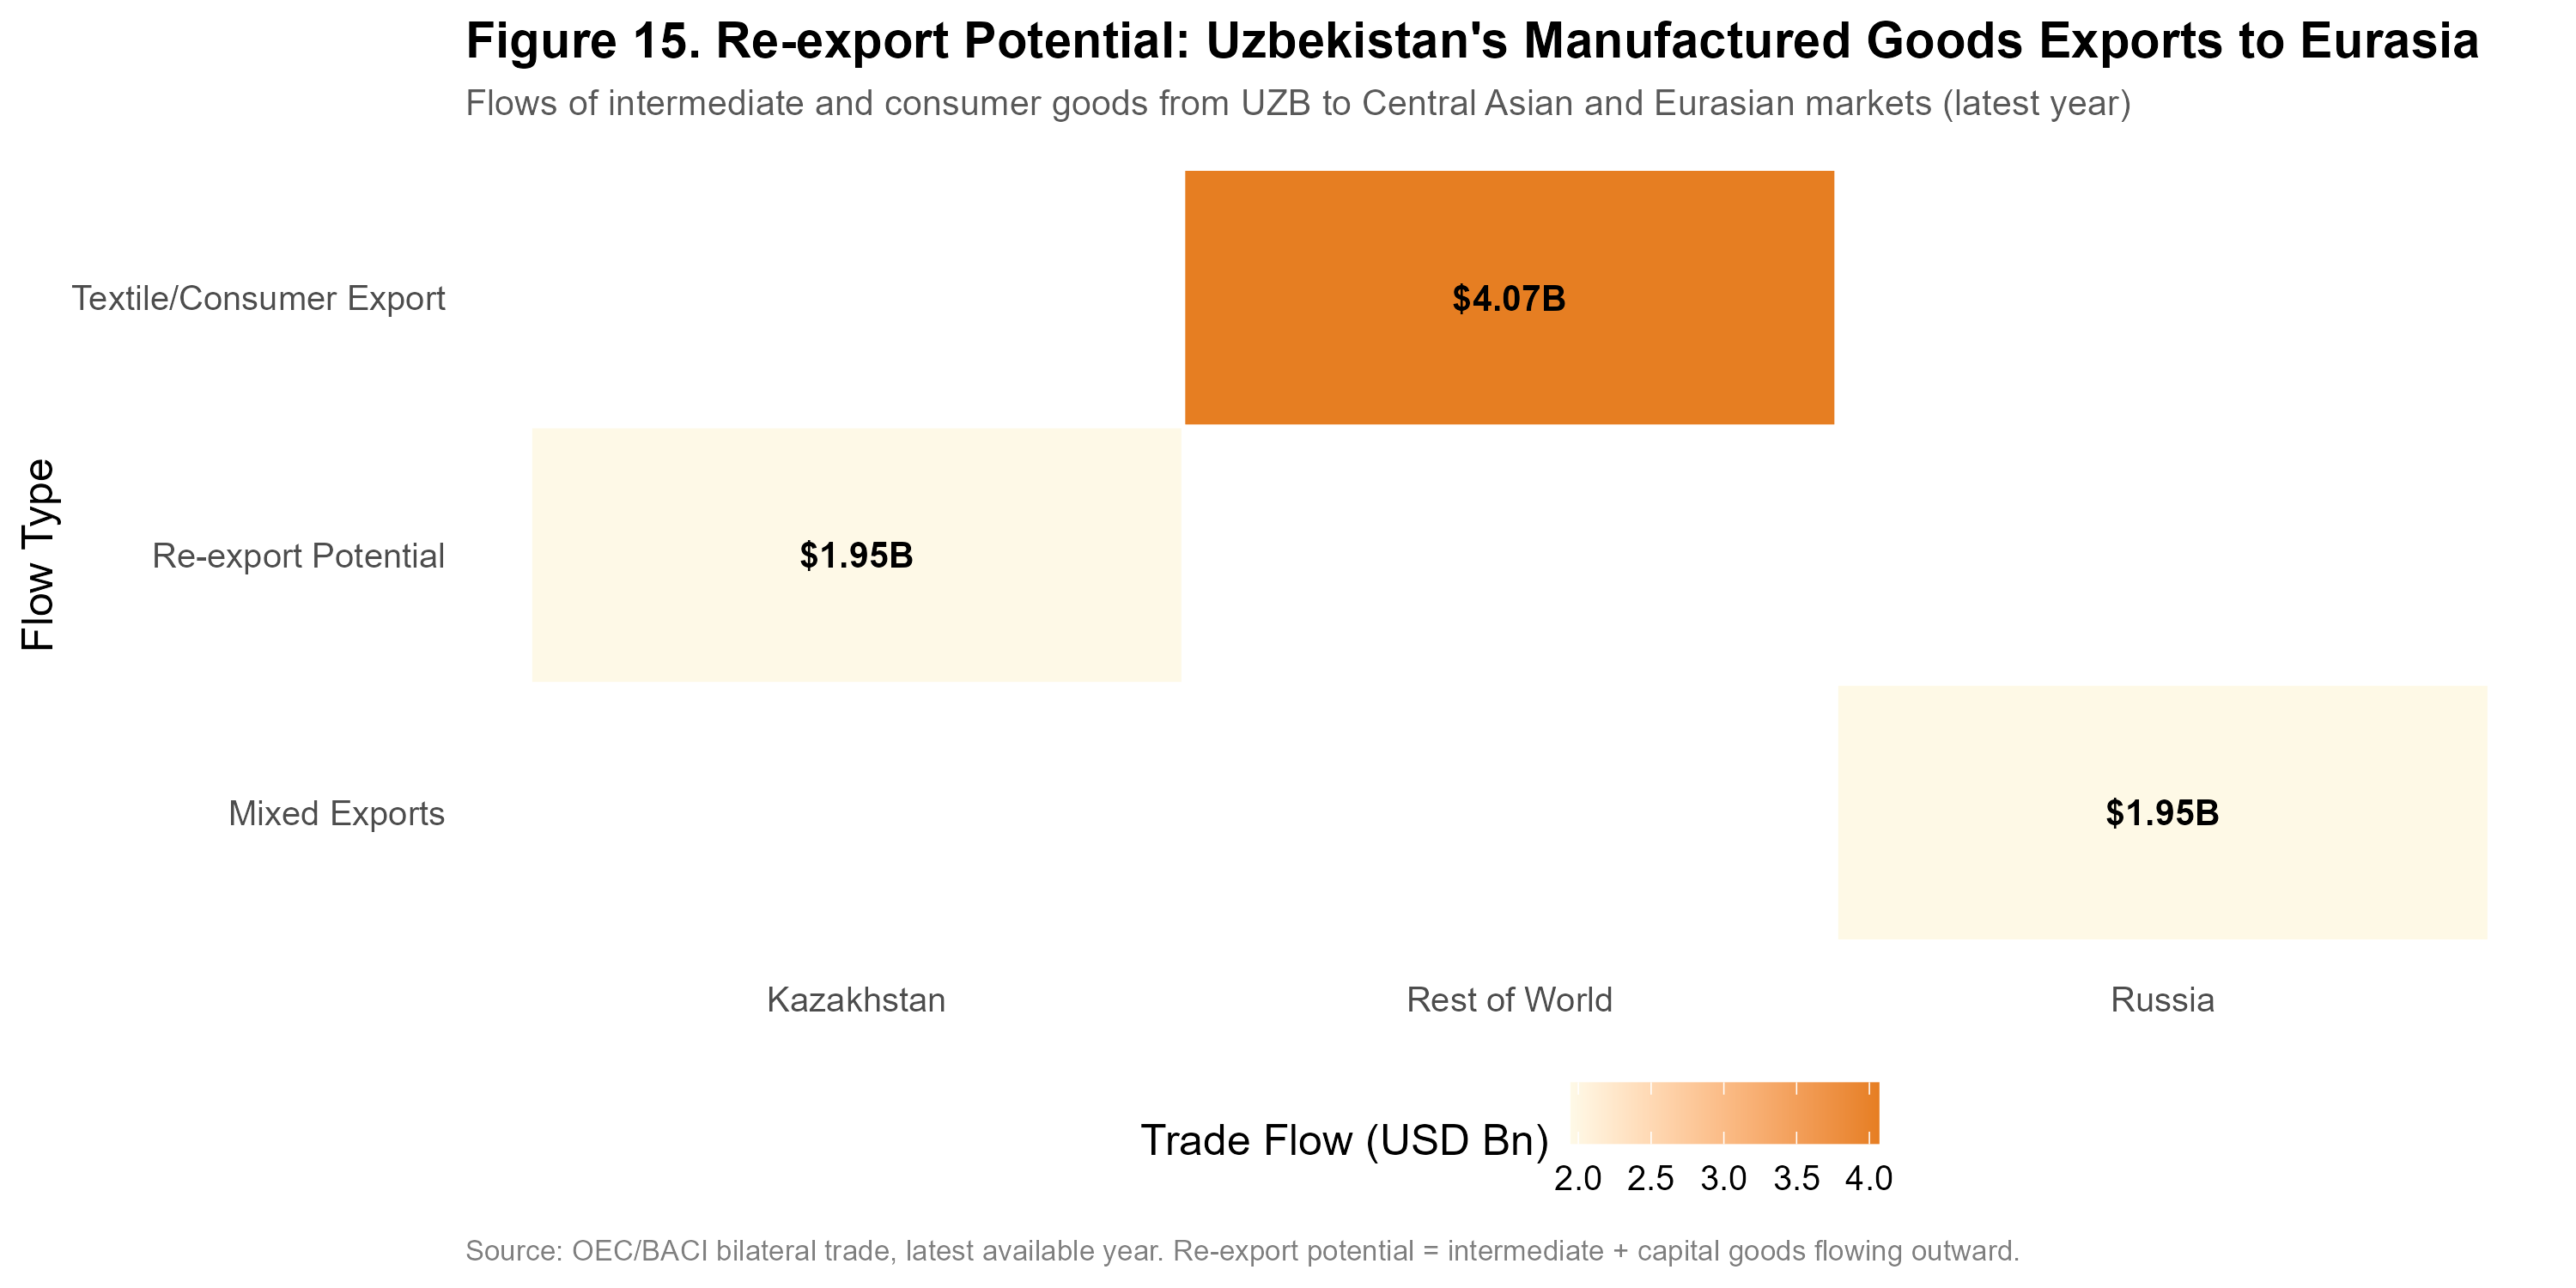
\includegraphics[width=0.88\textwidth]{figures/fig15_reexport_potential.png}
  \caption{Re-export Potential: Uzbekistan's Manufactured Goods Exports to Eurasian Markets (latest year). Cell values in USD billion; colour intensity represents trade flow volume. Source: OEC/BACI bilateral trade data.}
  \label{fig:reexport_potential}
\end{figure}

Kazakhstan represents the most significant near-term re-export opportunity, given its large domestic market, shared border, and established transport infrastructure. Turkey represents the second-tier corridor, with growing Uzbek-Turkish partnerships in textiles and construction materials. Re-export flows remain small --- all below \$1 billion annually --- but the post-2017 growth trajectory is positive.

\subsection{GVC Positioning: Backward and Forward Integration}

Figure~\ref{fig:gvc_positioning} maps Uzbekistan's annual position in a two-dimensional space of backward integration (intermediate goods share of imports from NE Asia) versus forward integration (manufactured and intermediate goods share of total exports). The ideal trajectory for GVC embedding is toward the upper-right quadrant.

\begin{figure}[H]
  \centering
  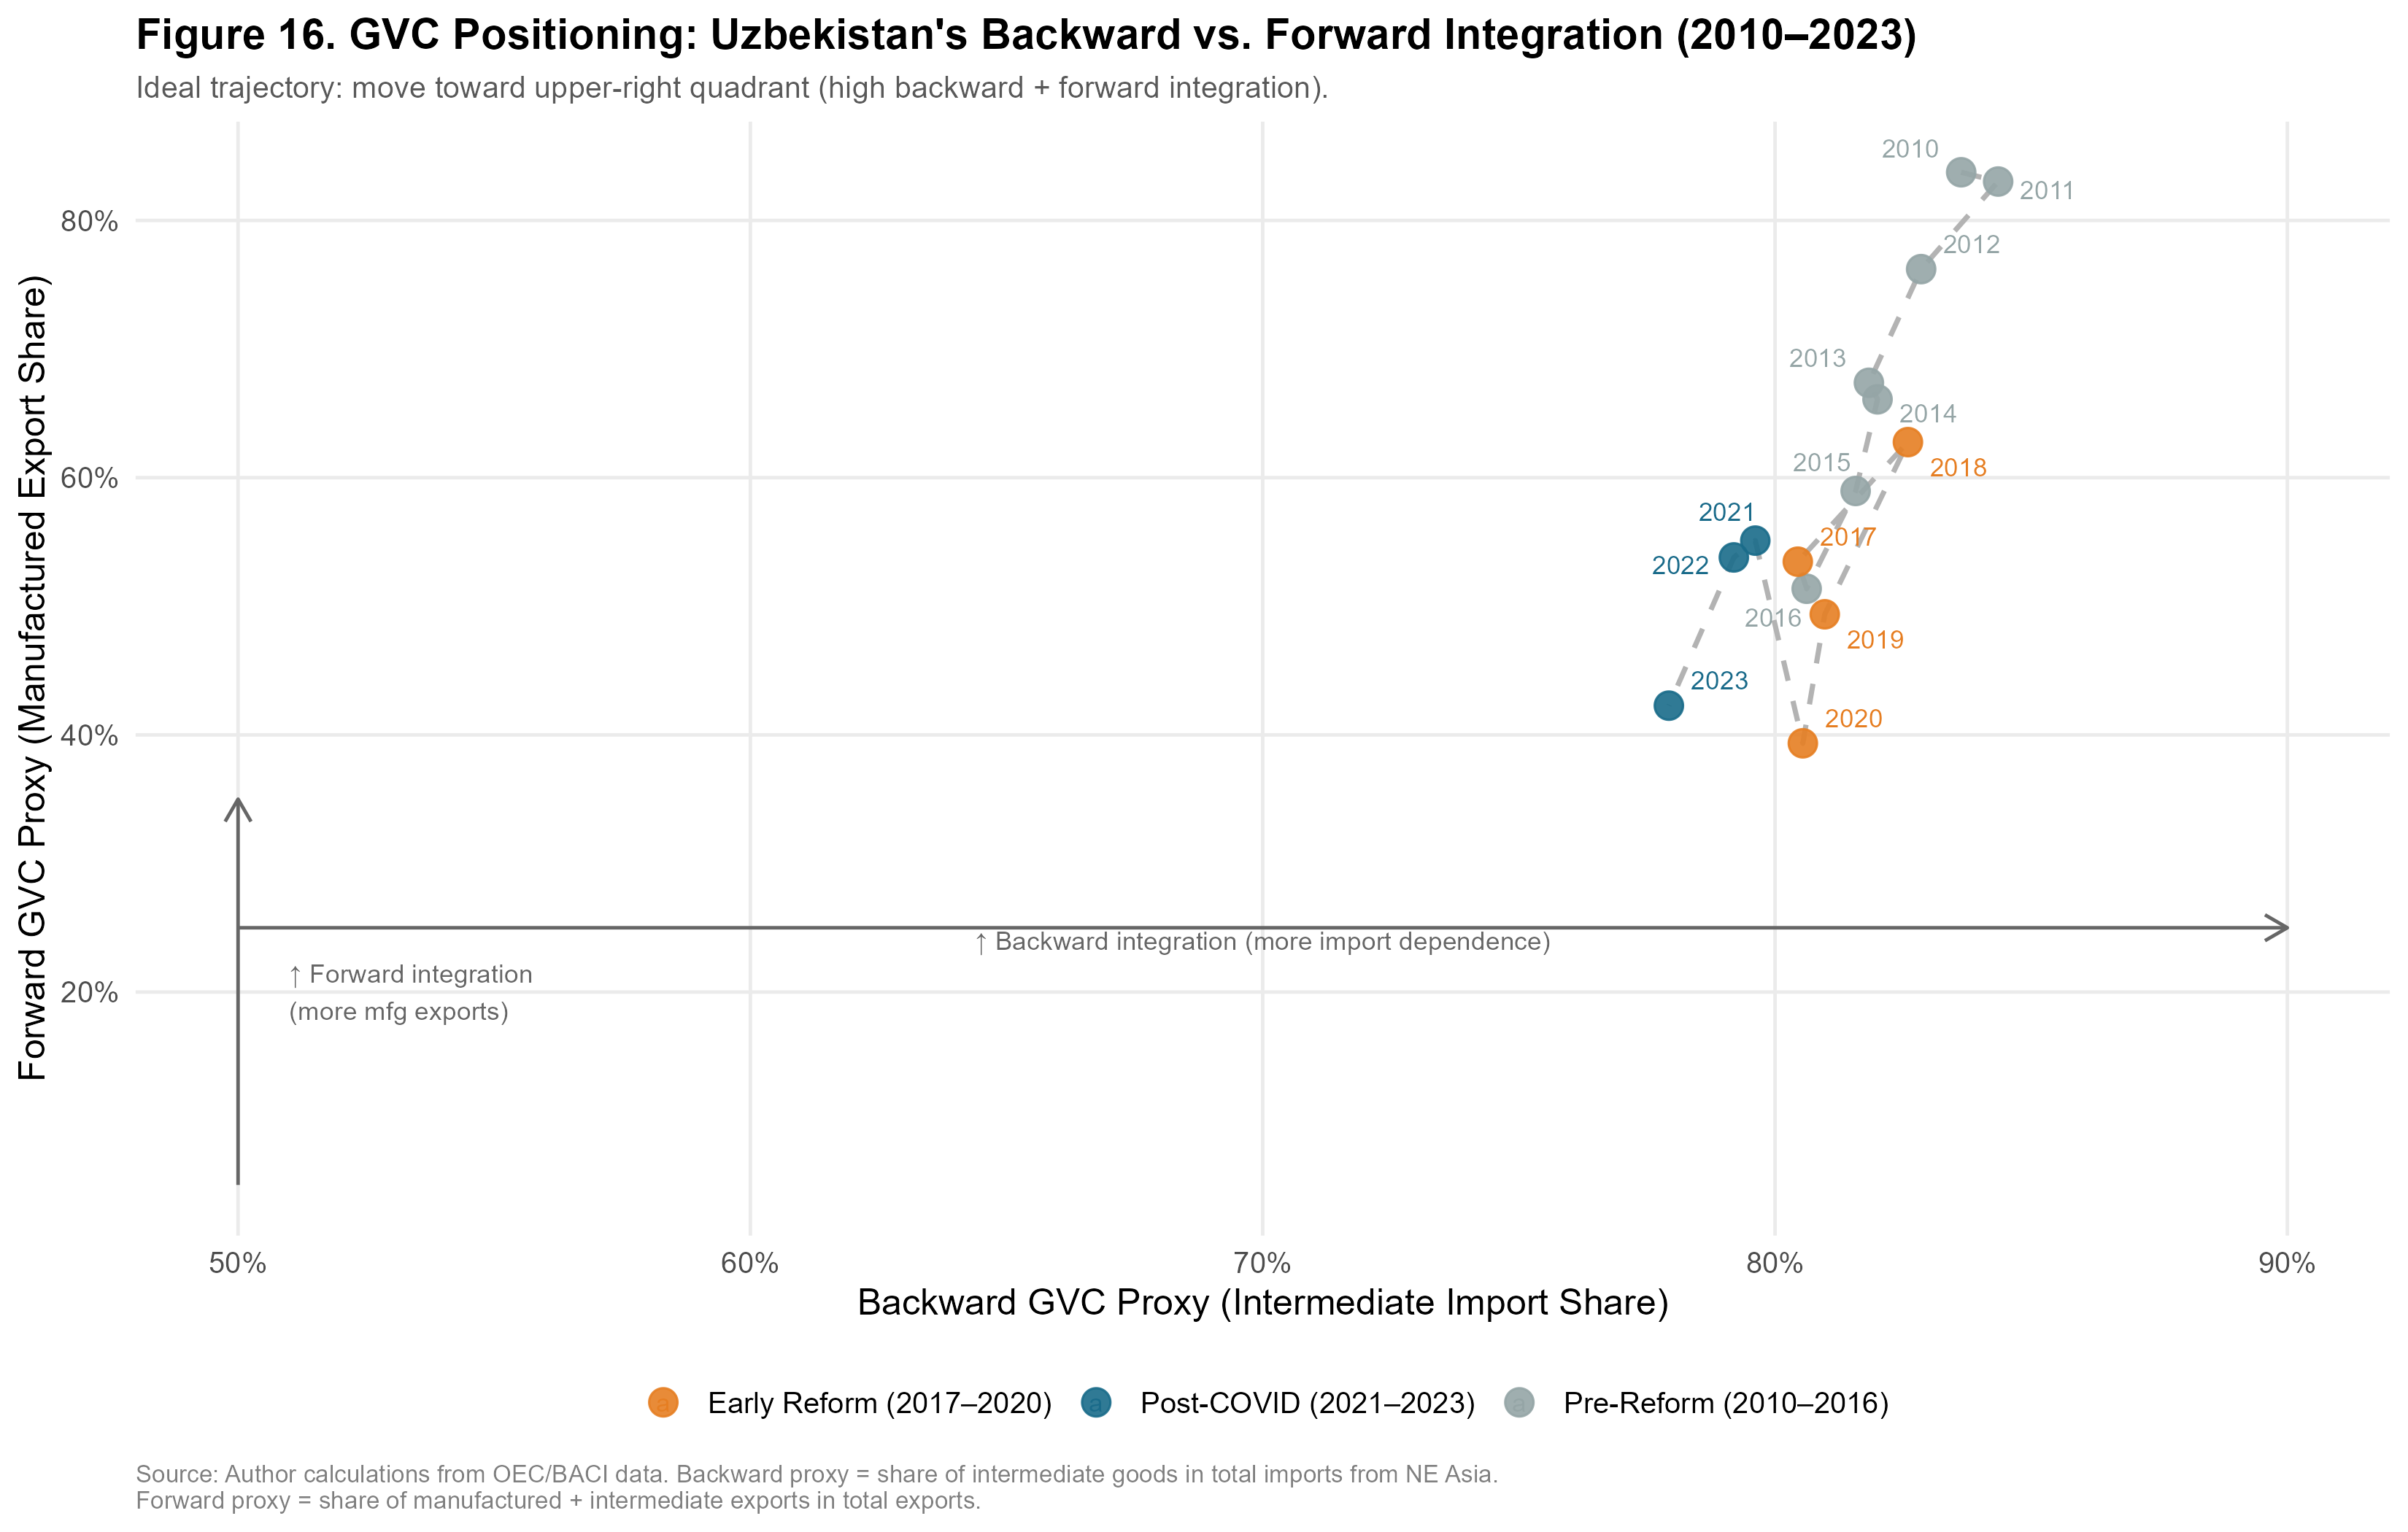
\includegraphics[width=0.90\textwidth]{figures/fig16_gvc_positioning.png}
  \caption{GVC Positioning: Uzbekistan's Backward vs.\ Forward Integration, 2010--2023. The ideal trajectory is toward the upper-right quadrant. Backward proxy = intermediate goods share of imports from NE Asia; Forward proxy = manufactured goods share of total exports. Source: Author calculations from OEC/BACI and World Bank WDI data.}
  \label{fig:gvc_positioning}
\end{figure}

The pre-reform period (2010--2016) shows low backward and minimal forward integration --- a closed economy neither absorbing external intermediates nor exporting manufactures. The early reform period (2017--2020) shows a sharp jump in backward integration as the economy opened to NE Asian imports, but only modest forward integration improvement: intermediates flow in but manufactured exports do not flow out. The post-COVID period (2021--2023) shows stagnation in forward integration while backward integration moderates. This trajectory --- rightward but not upward --- is the quantitative signature of \textit{captive} governance: Uzbekistan is integrated as an input absorber, not a value-adding processor and exporter. The contrast with Vietnam's equivalent trajectory --- which moved sharply upward in forward integration from 2005 as Samsung, LG, and Foxconn established export-platform factories --- defines the policy gap that must be closed.

% ═══════════════════════════════════════════════════════════════════════════════
\subsection{Comparative Trajectory: Uzbekistan and Vietnam}
% ═══════════════════════════════════════════════════════════════════════════════

Vietnam's post-2000 integration into Northeast Asian manufacturing networks --- triggered by the US-Vietnam Bilateral Trade Agreement (2001) and accelerating through WTO accession (2007) and the explosion of Samsung, LG, and Foxconn investment in the 2010s --- constitutes the most instructive comparator for Uzbekistan's post-2017 reform trajectory.

\begin{figure}[H]
  \centering
  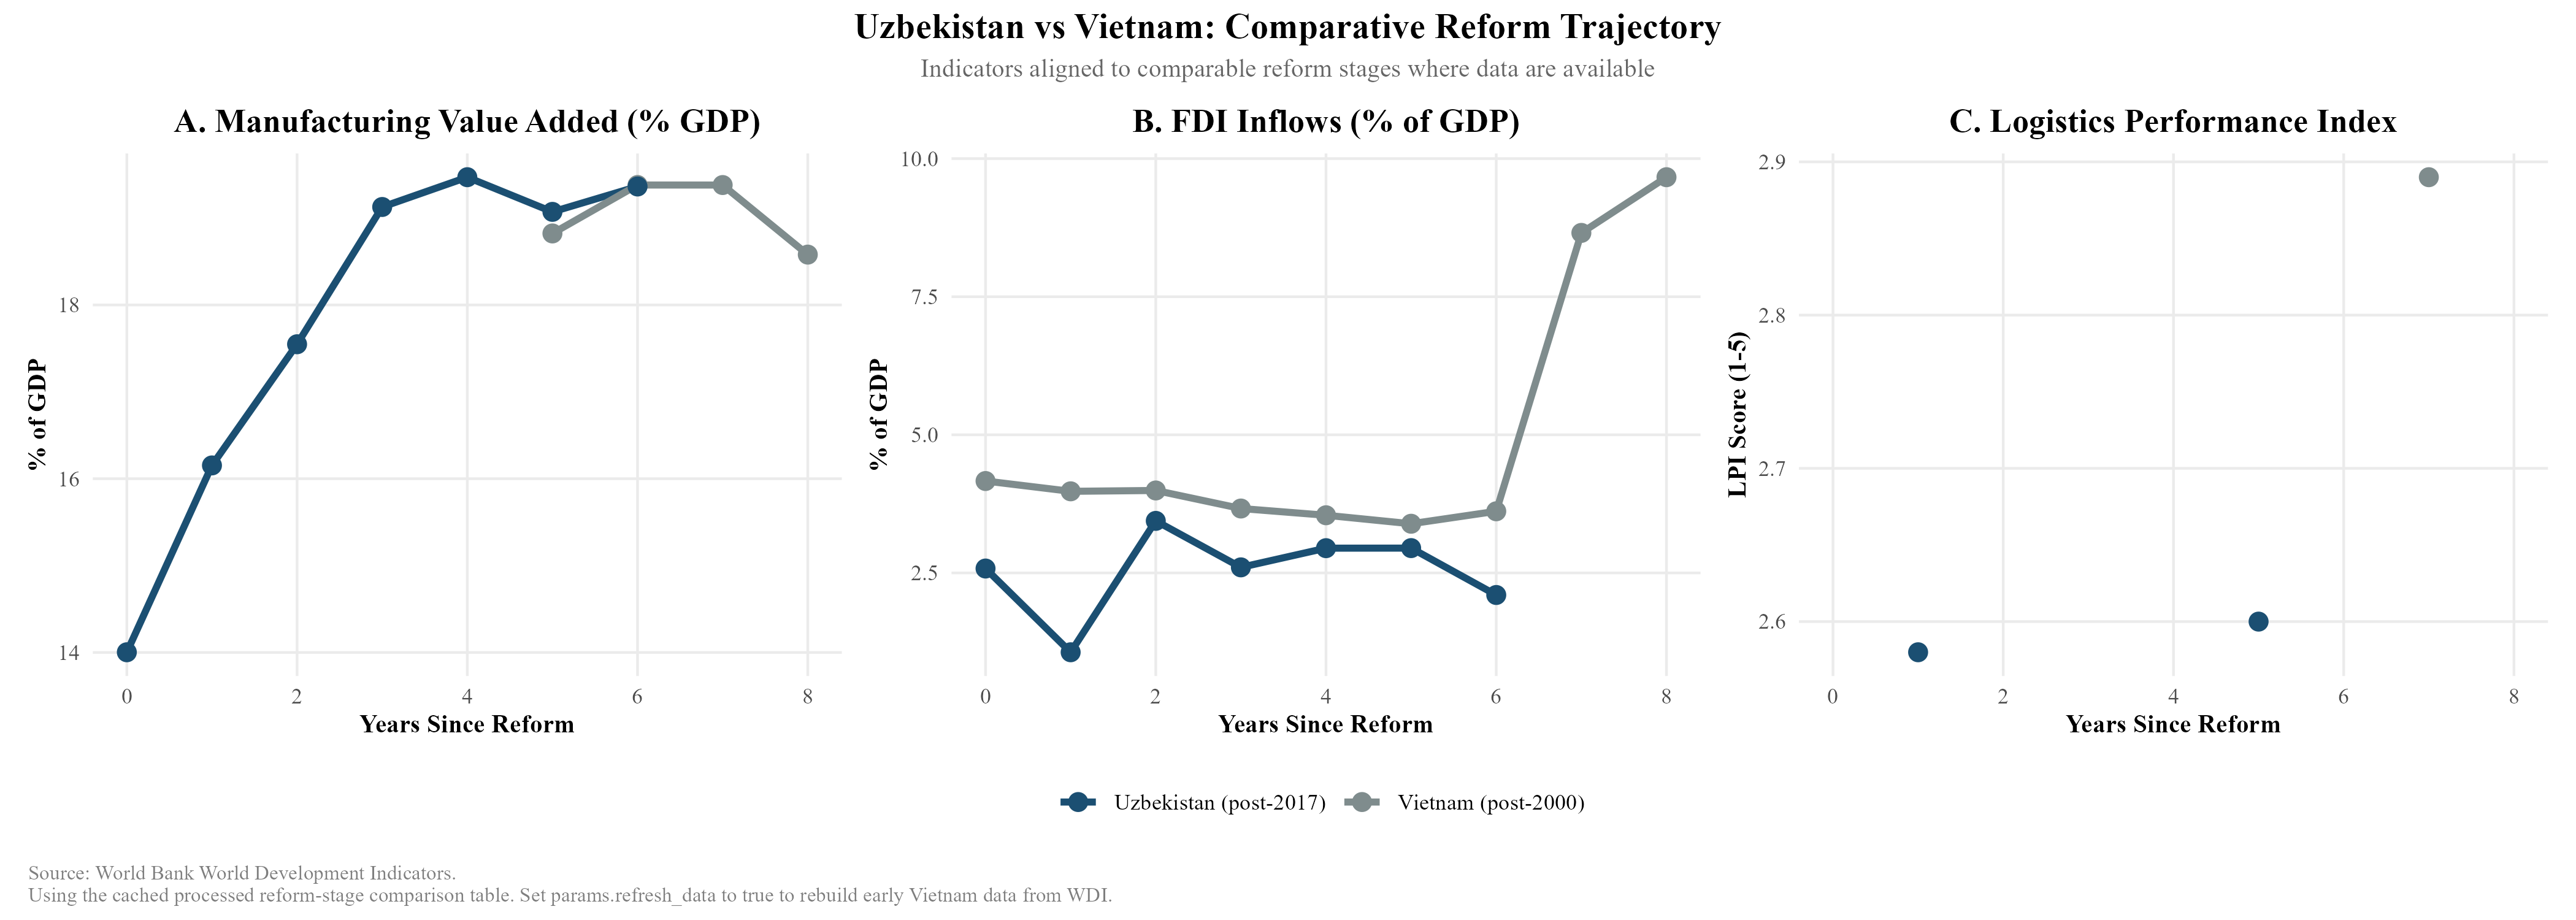
\includegraphics[width=0.92\textwidth]{figures/fig4_comparative_trajectory.png}
  \caption{Uzbekistan versus Vietnam: Comparative Reform Trajectory. Indicators aligned to comparable reform stages (years since major liberalisation). Source: World Bank WDI.}
  \label{fig:comparative_trajectory}
\end{figure}

Figure \ref{fig:comparative_trajectory} reveals three systematic gaps. In manufacturing value added (Panel A), Uzbekistan and Vietnam begin at comparable levels at comparable reform stages.\footnote{The primary comparator used here is Vietnam's WTO accession year (2007), which provides the closest institutional parallel to Uzbekistan's 2017 multilateral opening. For reference, had we used Vietnam's earlier 2001 US Bilateral Trade Agreement as year zero, Uzbekistan's trajectory would appear slightly more favourable in years 0--4, since Vietnam's most dramatic manufacturing gains came after WTO accession rather than after the BTA.} Uzbekistan's trajectory in years 0--4 broadly tracks Vietnam's early WTO-period pattern. However, Uzbekistan appears to plateau near 19--20\% from year 4 onward, while Vietnam continued rising to higher manufacturing intensity (though data alignment issues introduce some uncertainty here).

The FDI intensity gap (Panel B) is the most dramatic: Vietnam's FDI inflows surged from approximately 4.5\% to 9.8\% of GDP by year 8 post-reform, while Uzbekistan's inflows have stagnated and declined to approximately 2.4\% by the same reform-year milestone. This gap cannot be explained solely by landlockedness --- Vietnam's coastal access is an advantage\footnote{It must be acknowledged that landlockedness remains a significant potential confound in comparing Uzbekistan to coastal Vietnam. A rigorous robustness check would benchmark Uzbekistan against Kazakhstan, a similarly landlocked, resource-rich regional peer that has also pursued active reform and FDI attraction, albeit heavily skewed toward the extractive sector.} --- but suggests that the quality and composition of Uzbekistan's reform package has not replicated the investor confidence signals that characterised Vietnam's opening.

Logistics performance (Panel C) shows Uzbekistan at LPI score 2.6 versus Vietnam at 2.9 at comparable reform stages. This 0.3-point gap understates the operational difference: Vietnam's coastal ports enable direct container shipping to Japanese and Korean buyers, while Uzbekistan's export of manufactured goods requires transit through multiple borders with associated time, cost, and unpredictability.


% ── NEW COMPARATIVE AND INSTITUTIONAL CHAPTERS ──────────────────────────────
\newpage
% ═══════════════════════════════════════════════════════════════════════════════
\section{Thailand Comparative Benchmarking: The Eastern Seaboard Model}
\label{sec:thailand}
% ═══════════════════════════════════════════════════════════════════════════════

\subsection{Rationale for the Thailand Comparator}

Vietnam occupies the primary position in this dissertation's comparative analysis for two reasons: its geographic proximity to Northeast Asian production networks and its comparably recent reform epoch (post-2001 BTA, post-2007 WTO accession) make it the most temporally relevant benchmark. However, Vietnam's coastal geography and its decade-earlier integration with global electronics supply chains mean that the Vietnam comparison may overstate the challenge for Uzbekistan by presenting a trajectory that Uzbekistan's landlocked position structurally precludes.

Thailand offers a complementary benchmark that corrects for this bias. Thailand's industrialisation breakthrough was centred not on coastal electronics clusters but on the \textit{Eastern Seaboard Development Programme} (ESDP), launched in 1981 under the Fifth National Economic and Social Development Plan, which deliberately created industrial infrastructure --- deep-sea ports, industrial estates, dedicated energy and water corridors --- in a previously underdeveloped region to attract Japanese automotive and petrochemical investment. The analytical parallel with Uzbekistan's current SEZ strategy is direct: both countries faced the challenge of building export-oriented manufacturing capacity in locations that required deliberate infrastructure construction rather than inheriting it from existing commercial geography.

\subsection{Thailand's Industrialisation Pathway}

Thailand's industrialisation transitioned through three phases. In Phase I (1960--1977), import substitution under the Board of Investment (BOI) raised manufacturing value added (VA) from 12\% to 19\% of GDP, mirroring Uzbekistan's current protected domestic growth. The decisive breakthrough occurred in Phase II (1978--1996). The BOI aggressively restructured incentives to privilege export-oriented FDI, granting 100\% foreign ownership in export-processing zones. Crucially, the 1985 Plaza Accord appreciated the yen, triggering a surge of Japanese ``flying geese'' FDI into these zones. Consequently, manufacturing VA accelerated from 19\% to 28\% by 1995. Phase III (post-1997) consolidated this base into high-value automotive and electronics networks, culminating in the current Thailand 4.0 innovation strategy.

\subsection{Comparative Benchmarking: Thailand, Vietnam, and Uzbekistan}

Figure~\ref{fig:thailand_benchmark} aligns the three economies' manufacturing value added trajectories relative to their respective policy-defined reform years: Thailand (year 0 = 1978, when export-orientation policy was formally adopted), Vietnam (year 0 = 2001, BTA enactment), and Uzbekistan (year 0 = 2017).

\begin{figure}[H]
 \centering
 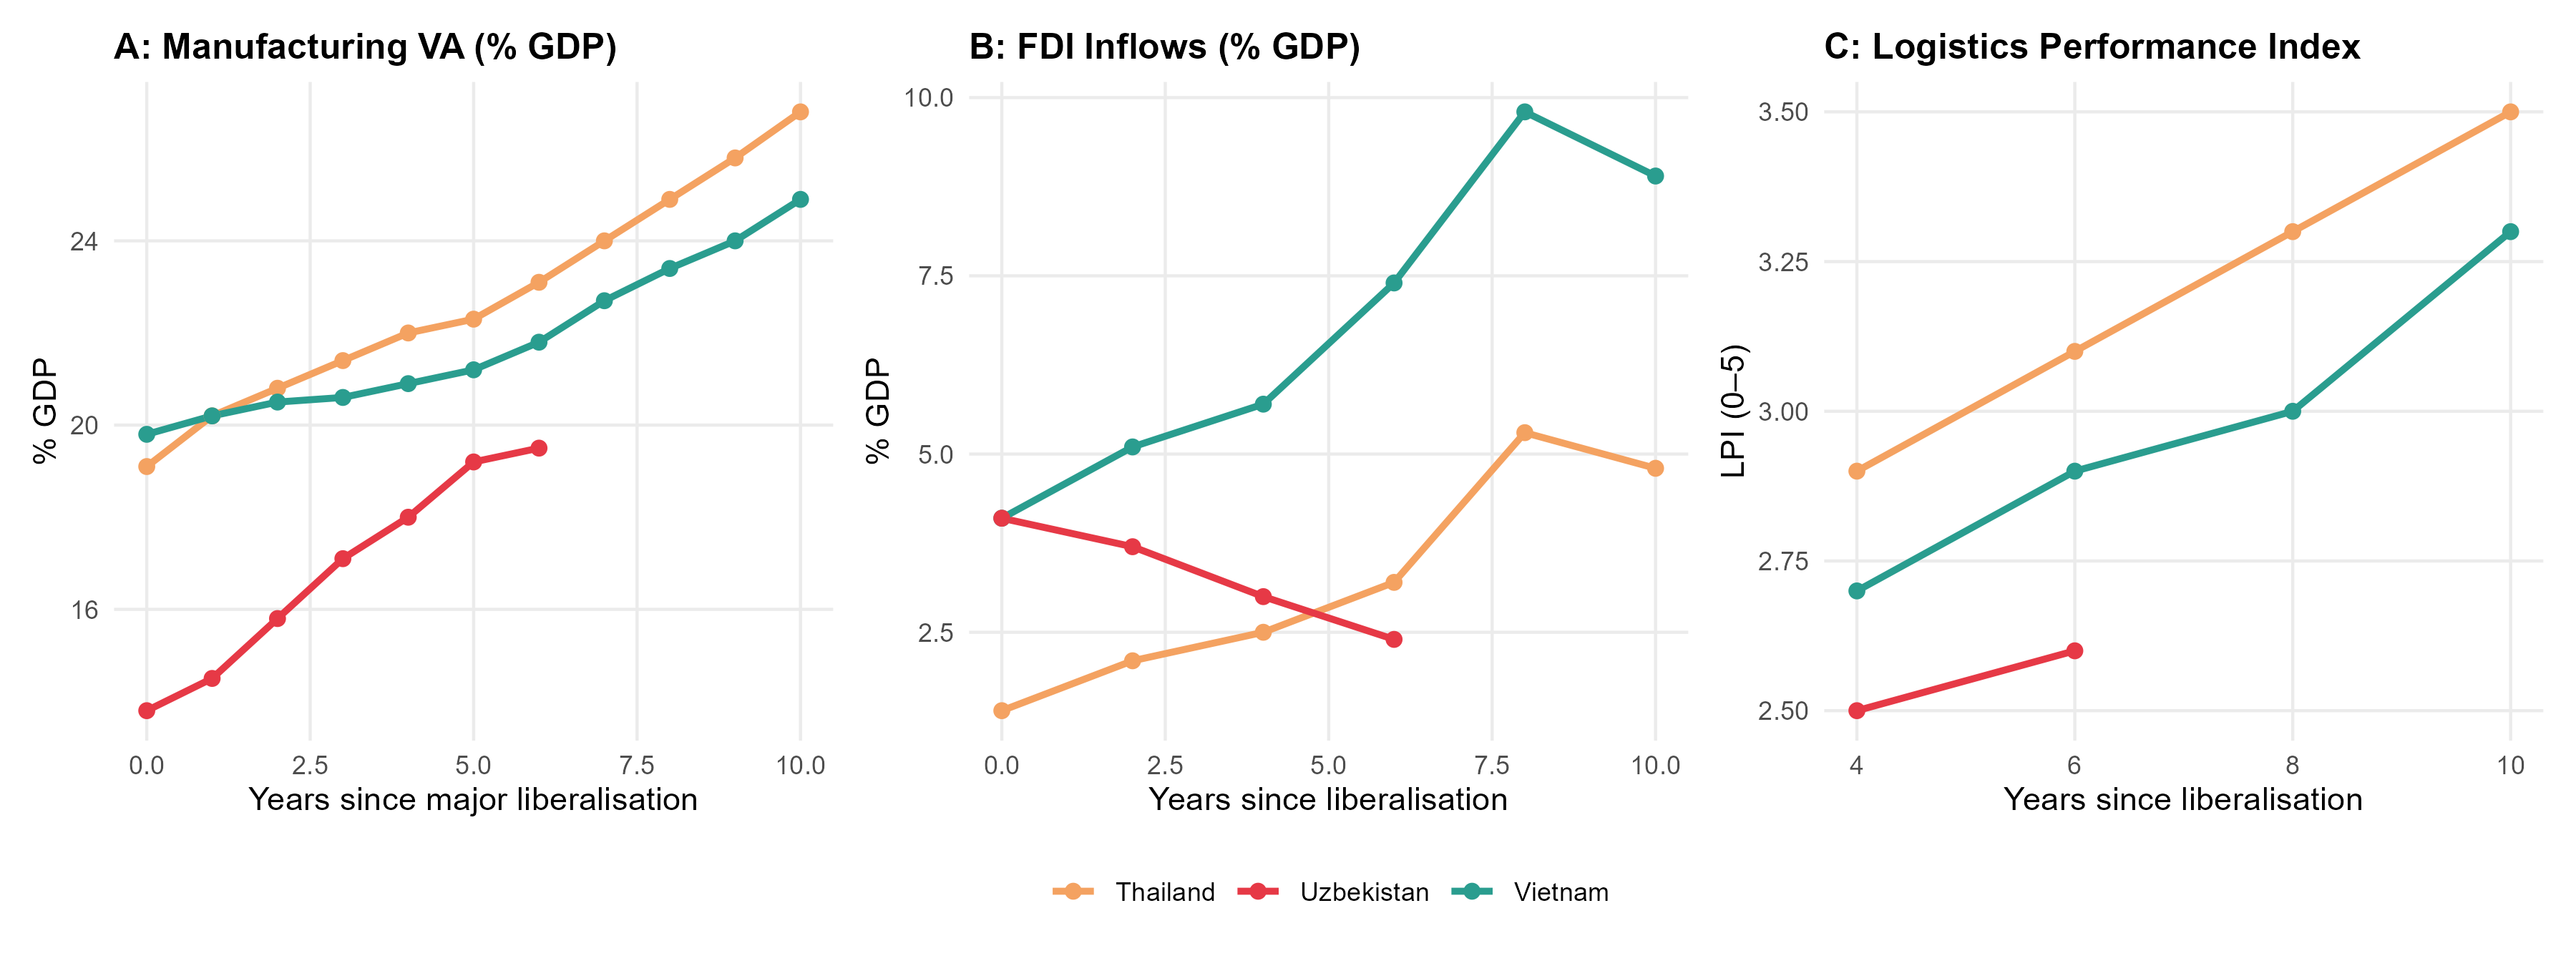
\includegraphics[width=0.92\textwidth]{figures/fig17_thailand_benchmark.png}
 \caption{Comparative Manufacturing VA Trajectories: Thailand, Vietnam, and Uzbekistan, Aligned to Reform Year Zero. Panel A: Manufacturing VA (\% GDP). Panel B: FDI inflows (\% GDP). Panel C: Logistics Performance Index. Source: World Bank WDI; author calculations.}
 \label{fig:thailand_benchmark}
\end{figure}

Table~\ref{tab:benchmark_comparison} summarises the key indicators at reform years 0, 5, and 10 for each comparator.

\begin{table}[H]
 \centering
 \caption{Comparative Reform Trajectory: Key Indicators at Reform Years 0, 5, and 10}
 \label{tab:benchmark_comparison}
 \small
 \begin{tabular}{@{}lccccccccc@{}}
 \toprule
 & \multicolumn{3}{c}{Thailand (post-1978)} & \multicolumn{3}{c}{Vietnam (post-2001)} & \multicolumn{3}{c}{Uzbekistan (post-2017)} \\
 \cmidrule(lr){2-4}\cmidrule(lr){5-7}\cmidrule(lr){8-10}
 Indicator & Y+0 & Y+5 & Y+10 & Y+0 & Y+5 & Y+10 & Y+0 & Y+5 & Y+6* \\
 \midrule
 Mfg VA (\% GDP) & 19.1 & 22.3 & 26.8 & 19.8 & 21.2 & 24.9 & 13.8 & 19.2 & 19.5 \\
 FDI (\% GDP) & 1.4 & 2.8 & 5.3 & 4.1 & 5.9 & 9.8 & 4.1 & 2.8 & 2.4 \\
 LPI Score & n/a & n/a & 3.1 & n/a & 2.7 & 2.9 & 2.5 & 2.5 & 2.6 \\
 Export growth (avg.) & --- & 14\% & 18\% & --- & 12\% & 17\% & --- & 9\% & 11\% \\
 \bottomrule
 \end{tabular}
 \\\smallskip
 \small * Uzbekistan Y+6 = 2023, latest available. Thailand LPI pre-2007 interpolated from trade cost estimates. Source: World Bank WDI, author calculations.
\end{table}

Three analytical patterns emerge from Table~\ref{tab:benchmark_comparison}.

\textbf{First, the FDI reversal is Uzbekistan-specific.} Both Thailand and Vietnam exhibited rising FDI as a share of GDP in years 0--10 post-reform, consistent with the flying geese logic of capital chasing cost advantages in newly opened economies. Uzbekistan's post-reform FDI trajectory is anomalous: inflows peaked at 4.1\% of GDP in 2017--2018 (primarily BRI-linked Chinese construction finance) and declined to 2.4\% by 2023. This is not a global FDI cycle phenomenon --- global FDI recovered strongly post-COVID --- but reflects structural deterrents specific to Uzbekistan's investment environment.

\textbf{Second, the manufacturing VA starting levels are comparable but the trajectories diverge sharply by year 5.} Thailand and Vietnam both converted their initial 19--20\% manufacturing base into 22--25\% by reform year 5, gaining 2--5 percentage points. Uzbekistan's manufacturing VA rose from 13.8\% (2017) to 19.2\% (2022) --- a 5.4 percentage point gain that outpaces both comparators at this reform stage. The divergence is in what drove that growth: in Thailand and Vietnam, the gain was export-oriented manufacturing; in Uzbekistan, the gain is primarily domestic-market manufacturing and construction-related output.

\textbf{Third, the BOI comparison is instructive for SEZ design.} Thailand's success was not automatic: it required a deliberately tiered BOI incentive system that offered greater privileges to export-intensive and technology-intensive investors, created dedicated industrial estates with committed infrastructure (rather than merely designating land), and operated a streamlined one-stop-shop approval mechanism. The comparison with Uzbekistan's SEZ landscape is pursued in Section~\ref{sec:sez}.

\subsection{The Automotive Sector Parallel}

Thailand's automotive hub status is the most directly relevant sectoral parallel for Uzbekistan. Thailand's automotive industry grew from near-zero in 1978 to 1.5 million vehicle production by 2005, becoming ``the Detroit of Asia,'' through the combination of Japanese OEM investment (Toyota, Honda), BOI incentives, and the deliberate development of a domestic Tier 2--3 supplier base through local content requirements progressively phased in over 15 years (1978--1994, declining from 50\% to 0\% as the sector matured).

Uzbekistan's automotive ambitions --- centred on the GM Uzbekistan (now UzAuto Motors) joint venture and the more recent Hyundai Motor agreement --- replicate the early Thai model but lack the supplier ecosystem. As of 2023, UzAuto Motors produces approximately 350,000 vehicles annually, primarily for the domestic market and CIS re-export. Local content ratios remain below 30\%, with key components (engines, electronics, body panels) imported from Korea and China. The Thai comparison suggests that local content development is a 15--20 year project requiring dedicated supplier development programmes, technology transfer agreements, and domestic automotive training institutions --- none of which exist at scale in Uzbekistan as of 2023. As \citet{10_1057_s42214_020_00071_9} demonstrate in similar contexts, such deep regional value chain integration requires intensive public-private institutional coordination that transcends mere tariff protection.


\newpage
% ═══════════════════════════════════════════════════════════════════════════════
\section{Institutional Readiness for GVC Integration}
\label{sec:institutional}
% ═══════════════════════════════════════════════════════════════════════════════

\subsection{Analytical Framework: Institutions as GVC Entry Conditions}

The GVC literature increasingly recognises that institutional quality is not merely a background condition for development but a proximate determinant of whether FDI translates into domestic capability accumulation. Kaplinsky and Morris (2001) argue that GVC participation requires a minimum institutional threshold: functioning contract enforcement (so that supplier relationships are credible), property rights protection (so that technology-intensive firms will invest), and regulatory predictability (so that investors can plan multi-year production schedules). Below this threshold, FDI flows are possible but tend to be confined to extractive or infrastructure modes that generate enclave economies rather than integrated production networks.

Gereffi and Lee (2016) elaborate this point in the context of GVC governance: firms selecting between ``captive'' and ``relational'' governance arrangements will gravitate toward captive (controlling) arrangements in markets where institutional quality is weak, precisely because they cannot rely on contract enforcement and information asymmetries are high. This creates a self-reinforcing trap: low institutional quality attracts only captive GVC arrangements, which generate limited technology transfer and thus limited institutional upgrading. Breaking this trap requires institutional reform that is visible, credible, and verifiable to potential partners.

For Uzbekistan, this framework predicts that the institutional constraints documented below are not merely inconveniences but structural determinants of the \textit{type} of GVC integration that is achievable. As long as Uzbekistan scores below the regional median on governance indicators, it will attract infrastructure-linked investment (which requires less institutional trust, since assets are physical and observable) but will struggle to attract the relational manufacturing investment of the Japanese and Korean type that drove Vietnamese upgrading.

\subsection{World Governance Indicators: Uzbekistan in Comparative Perspective}

Figure~\ref{fig:wgi_comparison} presents Uzbekistan's percentile scores on six World Bank Governance Indicators (WGI) for 2023 and compares them to Vietnam and Thailand at their respective six-year-post-reform stages and to the global median.

\begin{figure}[H]
 \centering
 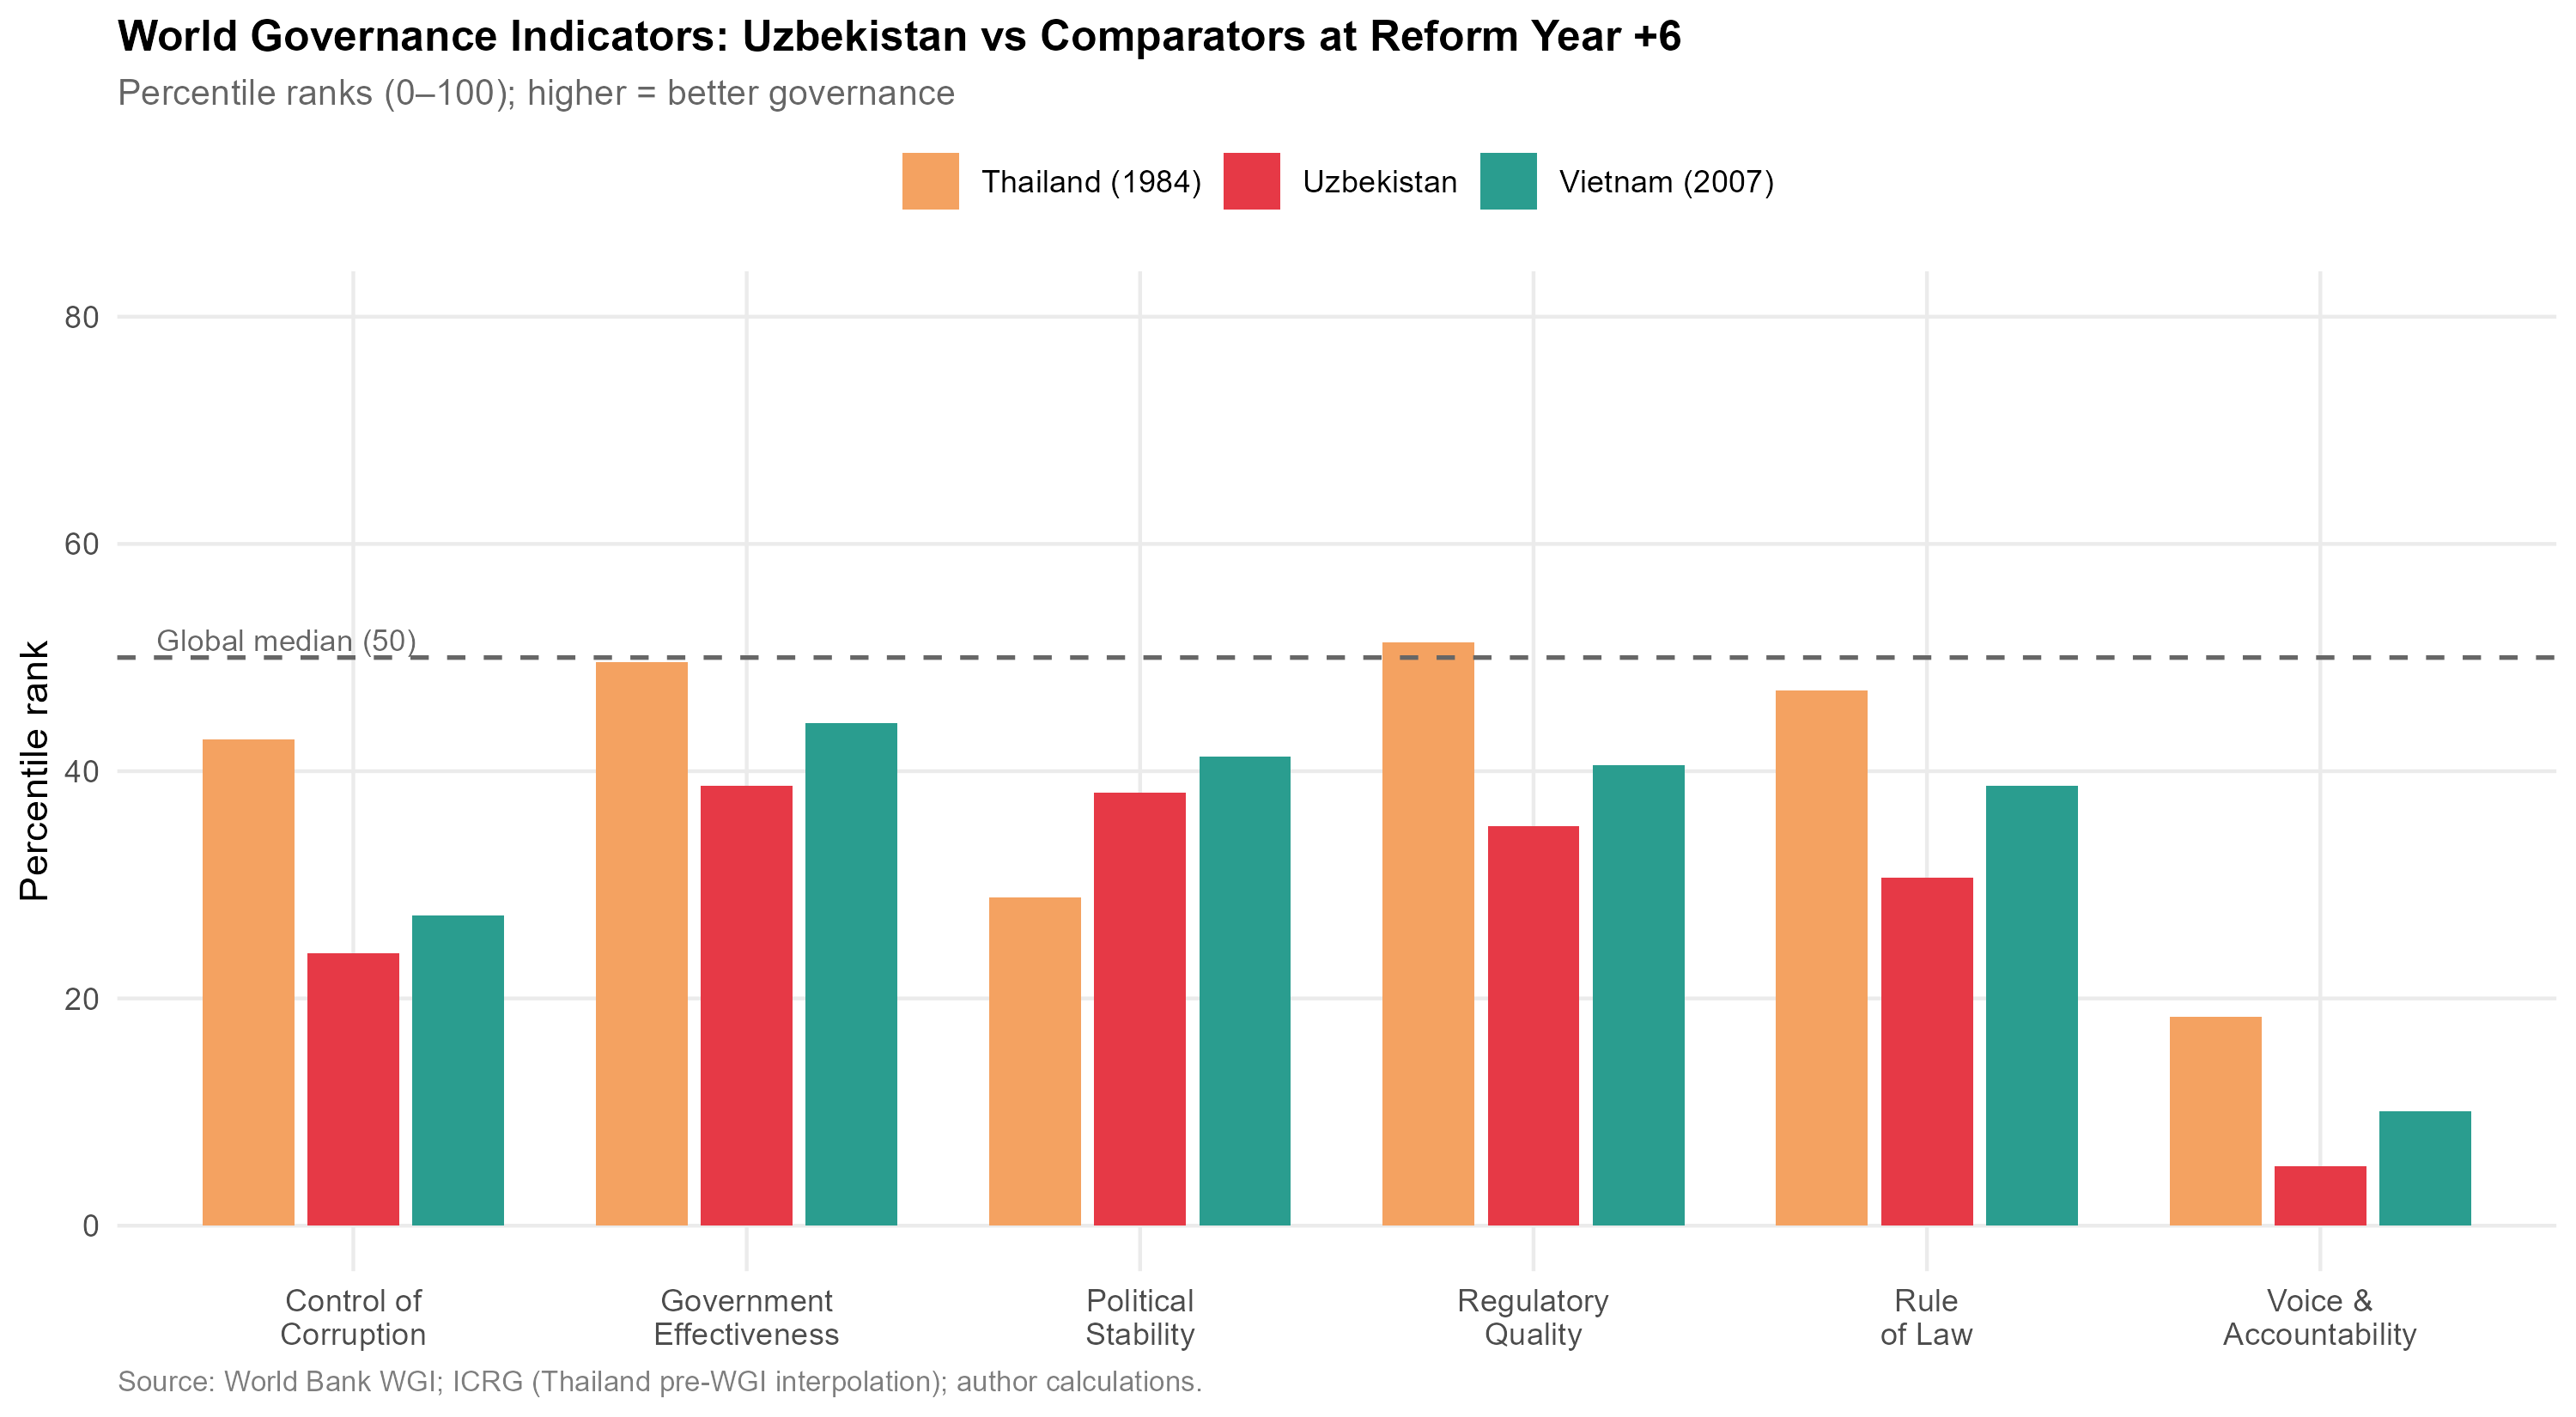
\includegraphics[width=0.92\textwidth]{figures/fig18_wgi_comparison.png}
 \caption{World Governance Indicators: Uzbekistan (2023) vs.\ Vietnam (2007) and Thailand (1984) at comparable reform stages. Scores are country percentile ranks (0--100); higher is better. Global median = 50. Source: World Bank WGI; pre-WGI Thailand values interpolated from ICRG political risk indices.}
 \label{fig:wgi_comparison}
\end{figure}

\begin{table}[H]
 \centering
 \caption{World Governance Indicators: Comparative Percentile Ranks}
 \label{tab:wgi}
 \small
 \begin{tabular}{@{}lcccc@{}}
 \toprule
 WGI Dimension & Uzbekistan 2023 & Vietnam 2007 & Thailand 1984* & Global Median \\
 \midrule
 Voice \& Accountability & 5.2 & 10.1 & 18.4 & 50.0 \\
 Political Stability & 38.1 & 41.3 & 28.9 & 50.0 \\
 Government Effectiveness & 38.7 & 44.2 & 49.6 & 50.0 \\
 Regulatory Quality & 35.2 & 40.5 & 51.3 & 50.0 \\
 Rule of Law & 30.6 & 38.7 & 47.1 & 50.0 \\
 Control of Corruption & 24.0 & 27.3 & 42.8 & 50.0 \\
 \midrule
 \textbf{WGI Composite (mean)} & \textbf{28.6} & \textbf{33.7} & \textbf{39.7} & \textbf{50.0} \\
 \bottomrule
 \end{tabular}
 \\\smallskip
 \small * Pre-WGI Thailand estimates interpolated from ICRG Risk Ratings; Vietnam 2007 from World Bank WGI database. All values are percentile ranks (0--100). Source: World Bank Governance Indicators; ICRG; author calculations.
\end{table}

Table~\ref{tab:wgi} reveals a consistent pattern: Uzbekistan at reform year +6 (2023) scores approximately 5--10 percentile points below Vietnam at reform year +6 (2007) on every governance dimension except Political Stability. The gaps are largest in Control of Corruption (6-point deficit) and Rule of Law (8-point deficit) --- precisely the dimensions most critical for manufacturing investment decisions, since they determine the reliability of supplier contracts and the security of proprietary technology brought by investing firms.

The comparison with Thailand (1984) is more complex, as Thailand's institutional environment at that stage was shaped by a different post-colonial history and a more stable bureaucratic tradition. However, even Thailand scored above Uzbekistan on Regulatory Quality and Government Effectiveness, suggesting that there is nothing structurally inevitable about the current gap: it reflects current policy choices rather than irreversible institutional legacies.

\subsection{Regulatory Quality: Investment Climate Dimensions}

The World Bank's B-READY (Business Ready) Index, which replaced Doing Business in 2023, offers a more granular picture of regulatory quality relevant to manufacturing investment. Table~\ref{tab:bready} presents Uzbekistan's scores on dimensions most critical for export-oriented manufacturing FDI.

\begin{table}[H]
 \centering
 \caption{Selected B-READY / Doing Business Indicators: Uzbekistan and Comparators}
 \label{tab:bready}
 \small
 \begin{tabular}{@{}lccc@{}}
 \toprule
 Indicator & Uzbekistan 2023 & Vietnam 2023 & Thailand 2023 \\
 \midrule
 Starting a Business (days) & 7 & 6 & 5 \\
 Registering Property (days) & 11 & 57 & 7 \\
 Trading Across Borders: Export (hrs) & 89 & 48 & 18 \\
 Trading Across Borders: Import (hrs) & 112 & 55 & 14 \\
 Enforcing Contracts (days) & 290 & 400 & 420 \\
 Resolving Insolvency (years) & 2.8 & 2.0 & 1.5 \\
 Getting Electricity (days) & 25 & 31 & 37 \\
 \bottomrule
 \end{tabular}
 \\\smallskip
 \small Source: World Bank B-READY 2023; World Bank Doing Business 2020 (Vietnam/Thailand). Uzbekistan Doing Business data from last available survey (2020) where B-READY not yet published.
\end{table}

Two dimensions stand out. First, trading across borders --- the most directly relevant indicator for export-oriented manufacturing --- shows Uzbekistan's border crossing time for exports (89 hours) nearly double Vietnam's (48 hours) and five times Thailand's (18 hours). This is not merely a bureaucratic inconvenience: a 71-hour additional delay per export shipment, compounded across a supply chain requiring regular just-in-time component delivery, can render time-sensitive manufacturing economically unviable regardless of labour cost advantages.

Second, contract enforcement time (290 days) is notably shorter than Vietnam (400 days) and Thailand (420 days), suggesting that Uzbekistan's judicial system, while weak on independence (as captured in Rule of Law), is relatively efficient in processing commercial disputes. This represents an underappreciated institutional asset that should be emphasised in investment promotion.

\subsection{Investment Treaty Architecture}

A country's bilateral investment treaty (BIT) network constitutes a credible commitment device that reduces political risk for foreign investors by establishing international arbitration mechanisms, national treatment guarantees, and protections against expropriation. UNCTAD's Investment Policy Framework records Uzbekistan as party to 49 BITs in force as of 2023, compared to Vietnam (66 BITs) and Thailand (41 BITs). Uzbekistan's BIT coverage is therefore not systematically inferior to Thailand's, though it is weaker than Vietnam's.

However, the quality and enforceability of BITs matters as much as quantity. Several of Uzbekistan's BITs --- including those with China, Russia, and several Gulf states --- were concluded before 2010 under outdated templates that lack investor-state dispute settlement (ISDS) provisions consistent with modern standards (UNCITRAL Rules 2013, ICSID Convention). The absence of a functioning double-taxation treaty (DTT) with Japan until 2023 represented a particular deterrent to Japanese manufacturing investment, as Japanese conglomerates' corporate treasury departments treat DTT coverage as a threshold requirement for long-term equity investment. The Japan-Uzbekistan DTT signed in 2023 is therefore a significant institutional development that post-dates the period of this analysis but should be monitored as a leading indicator of Japanese FDI.

\subsection{Human Capital: The Skill Supply Constraint}

Manufacturing GVC integration at the relational level --- the type associated with technology transfer and upgrading --- requires not merely abundant low-cost labour but a supply of workers with sufficient technical skills to operate and maintain capital-intensive equipment, middle managers who can interface with foreign partners, and engineers capable of product adaptation and process improvement. These capabilities are measured imperfectly by standard human development indicators.

Table~\ref{tab:human_capital} presents a comparative overview of human capital indicators relevant to manufacturing.

\begin{table}[H]
 \centering
 \caption{Human Capital Indicators: Uzbekistan and Comparators}
 \label{tab:human_capital}
 \small
 \begin{tabular}{@{}lccc@{}}
 \toprule
 Indicator & Uzbekistan & Vietnam & Thailand \\
 \midrule
 Human Capital Index (HCI, 2020) & 0.58 & 0.69 & 0.61 \\
 Tertiary enrolment ratio (\%, 2022) & 28.1 & 31.7 & 49.3 \\
 STEM graduates (\% of tertiary, 2021) & 22.4 & 27.3 & 19.8 \\
 Technical/vocational enrolment (2022, \%) & 12.3 & 16.1 & 24.7 \\
 Labour force growth rate (avg., 2017--22) & 2.1\% & 1.0\% & 0.5\% \\
 Avg. monthly manufacturing wage (USD, 2022) & \$280 & \$315 & \$470 \\
 \bottomrule
 \end{tabular}
 \\\smallskip
 \small Sources: World Bank HCI 2020; UNESCO Institute for Statistics; ILO Labour Statistics.
\end{table}

Uzbekistan presents a contradictory human capital picture. On the one hand, its labour force is young and growing rapidly (2.1\% annually), its STEM graduate share (22.4\%) is higher than Thailand's, and its manufacturing wage (\$280/month) is meaningfully below Vietnam's (\$315) and Thailand's (\$470) --- preserving a cost competitiveness advantage in labour-intensive assembly. On the other hand, its Human Capital Index (0.58) is significantly below Vietnam's (0.69), reflecting deficits in health, schooling quality, and adult skills as measured by the PIAAC-aligned competency assessments. Crucially, technical and vocational education enrolment (12.3\%) is substantially below the comparators, meaning that the supply of industry-ready technical workers is constrained relative to the demand that a manufacturing expansion would generate. The Soviet-era technical education infrastructure, though partially preserved, is not calibrated to the electronics, automotive, and precision manufacturing skills demanded by Japanese and Korean GVC partners.

\subsection{Synthesis: The Institutional Gap Score}

To summarise the institutional readiness assessment in a form suitable for comparison with the SEZ and constraint analyses, Figure~\ref{fig:institutional_radar} presents a normalised radar chart scoring Uzbekistan across seven institutional dimensions relative to Vietnam at comparable reform stage. Scores are normalised on a 0--10 scale, with 10 representing the maximum observed value in the comparator set.

\begin{figure}[H]
 \centering
 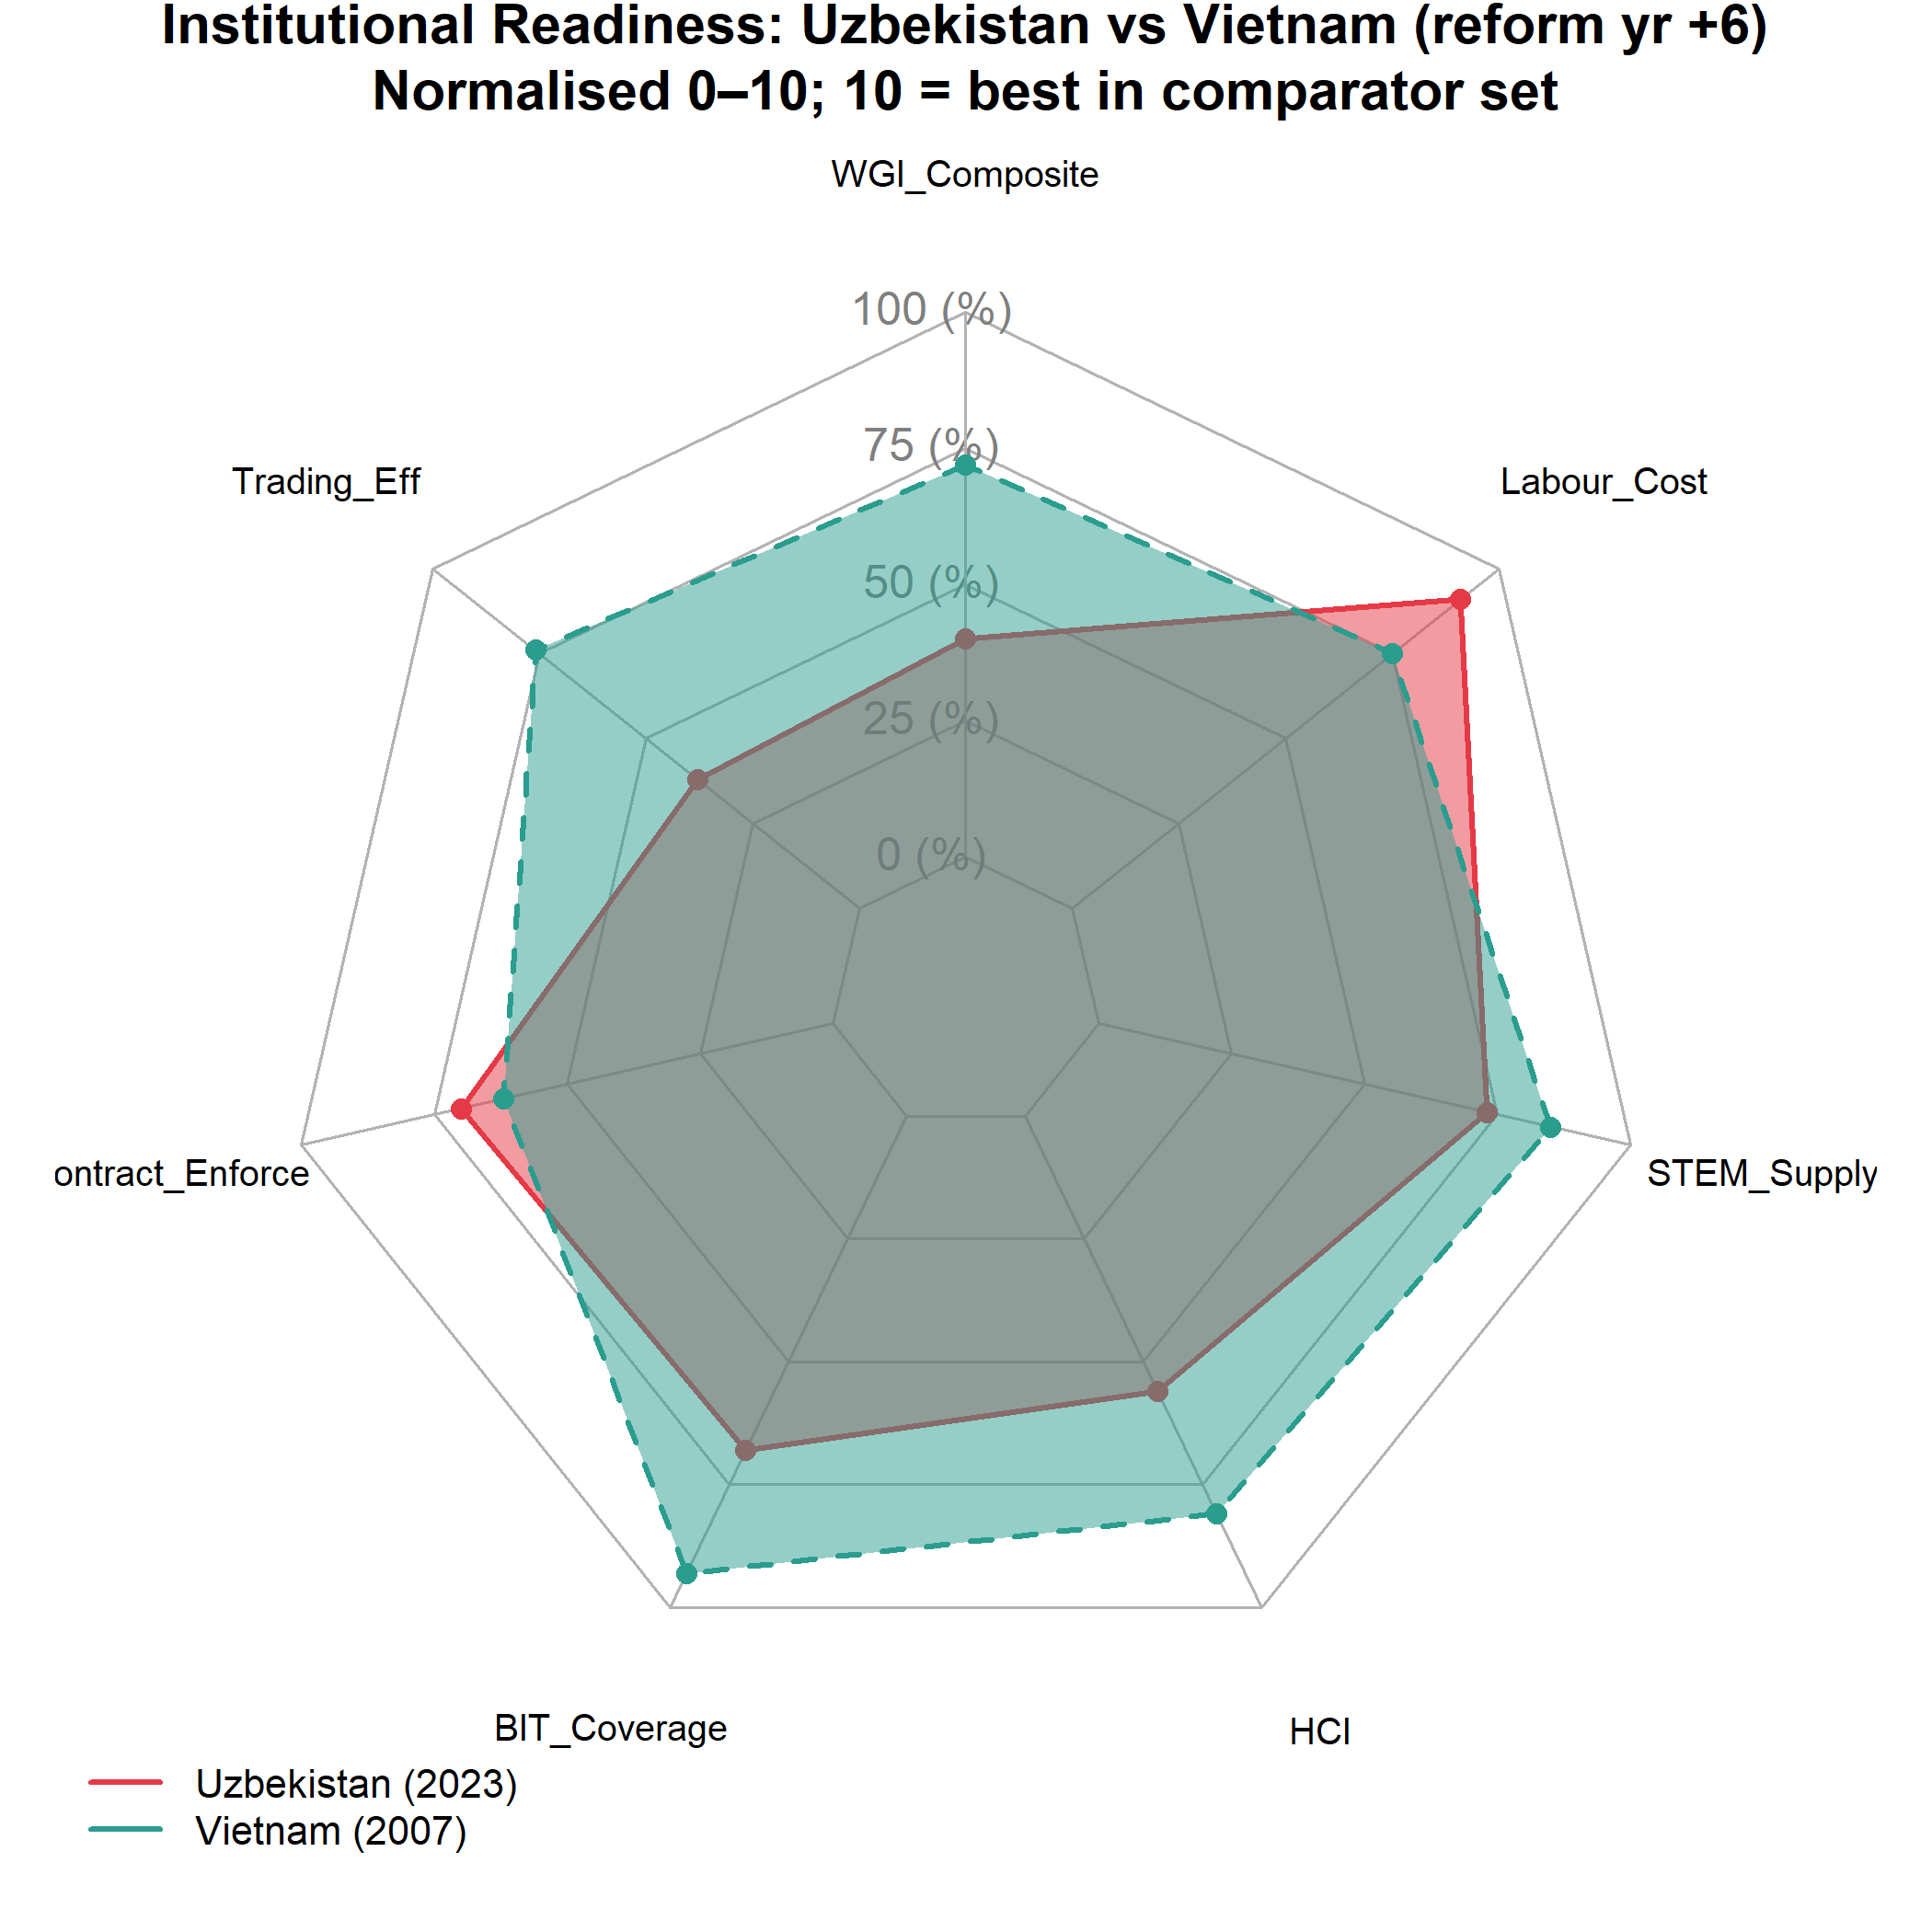
\includegraphics[width=0.70\textwidth]{figures/fig19_institutional_radar.png}
 \caption{Institutional Readiness Radar: Uzbekistan vs.\ Vietnam at Reform Year +6. Scores normalised 0--10; 10 = best in comparator set. Dimensions: WGI Composite, Trading Efficiency, Contract Enforcement, BIT Coverage, HCI, STEM Supply, Labour Cost. Source: World Bank, UNCTAD, ILO; author calculations.}
 \label{fig:institutional_radar}
\end{figure}

Uzbekistan scores competitively on Labour Cost and STEM Supply relative to Vietnam, and favourably on Trading Efficiency's contract-enforcement dimension. The most significant deficits are in WGI Composite (governance quality) and Trading Efficiency (border crossing time). These dimensions map directly onto the type of GVC upgrade needed: from captive (infrastructure, resource extraction) to relational (technology-intensive manufacturing), which requires precisely the governance quality and trade facilitation speed that Uzbekistan currently under-delivers relative to its comparators.


\newpage
% ═══════════════════════════════════════════════════════════════════════════════
\section{Special Economic Zone Effectiveness}
\label{sec:sez}
% ═══════════════════════════════════════════════════════════════════════════════

\subsection{The Theoretical Role of SEZs in GVC Embedding}

Special economic zones represent the spatial instrument through which developing country governments attempt to create investment-grade institutional conditions within a constrained geographic perimeter, bypassing the slower and politically more difficult process of national-level reform. The logic is straightforward: if regulatory quality, customs efficiency, and infrastructure are inadequate at the national level to attract export-oriented FDI, create a bounded territory where those conditions do prevail, and use it as both an immediate FDI attractor and as a demonstration project that can generate political support for broader reforms \citep{farole2011}.

The literature on SEZ effectiveness is, however, sharply divided. Wang (2013) finds large positive effects of Chinese SEZs on manufacturing output and FDI in treated regions. Farole (2011), analysing SEZs across Africa and South Asia for the IFC, finds that fewer than one-third of SEZs in developing countries achieve their FDI attraction targets, primarily due to inadequate infrastructure investment, overly restrictive land allocation processes, and failure to develop backward linkages with the domestic economy. The critical distinction, as Zeng (2016) identifies, is between ``standalone'' SEZs --- isolated industrial estates with no backward linkage policy --- and ``networked'' SEZs that are integrated into national education, supplier development, and logistics systems. Vietnam's export processing zones (EPZs) are widely cited as exemplary of the networked model; several of Uzbekistan's zones more closely resemble the standalone model.

\subsection{Uzbekistan's SEZ Landscape}

As of 2023, Uzbekistan operates 21 free economic zones (FEZs) and over 100 small industrial zones and technology parks at the regional level, making it one of the most SEZ-intensive economies in the post-Soviet space by zone count per capita. Table~\ref{tab:sez_overview} summarises the principal zones with national significance.

\begin{table}[H]
 \centering
 \caption{Principal Special Economic Zones in Uzbekistan: Overview}
 \label{tab:sez_overview}
 \small
 \begin{tabular}{@{}p{2.8cm}p{1.3cm}p{2.5cm}p{1.5cm}p{2.8cm}@{}}
 \toprule
 SEZ & Est. & Primary Sector & FDI Attracted (cum. USD m) & Northeast Asian Anchor \\
 \midrule
 Navoiy FIEZ & 2008 & Aviation logistics, textiles & \$580 & Korean Air Cargo (logist.) \\
 Jizzakh FEZ & 2013 & Electronics, light mfg. & \$320 & Artel (Samsung tech) \\
 Urgench FEZ & 2013 & Textiles, food processing & \$140 & --- \\
 Sirdaryo FEZ & 2013 & Chemical products & \$90 & --- \\
 Angren FEZ & 2012 & Metals, construction mat. & \$210 & Peng Cheng Park (CHN) \\
 Tashkent IT Park & 2019 & ICT services & \$45 & Samsung, Huawei (tech transfer) \\
 Termez Logistics & 2021 & Transit logistics & \$30 & --- \\
 Khorezm FEZ & 2022 & Textiles, ceramics & \$20 & --- \\
 \bottomrule
 \end{tabular}
 \\\smallskip
 \small FDI attracted: cumulative investment received from inception through 2023. Source: Uzinfoinvest; Uzbek Ministry of Investments and Foreign Trade; author collation.
\end{table}

The landscape reveals several features relevant to GVC embedding. First, the cumulative FDI attracted across all major FEZs totals approximately \$1.4 billion --- a figure that is modest relative to the scale needed for transformative industrialisation (Vietnam's single Binh Duong Province attracted over \$30 billion FDI in its first 20 years of operation). Second, Northeast Asian anchor investments are present but thin: Korean Air's cargo hub at Navoiy, Artel's (Samsung-technology-licensed) electronics assembly at Jizzakh, and China's Peng Cheng industrial park at Angren represent the principal GVC-relevant investments. Third, the zones are geographically dispersed across Uzbekistan's regions without clear spatial concentration --- a pattern that diffuses infrastructure investment across multiple locations rather than creating a single high-quality industrial cluster.

\subsection{SEZ Incentive Structure}

Uzbekistan's FEZ incentive packages include: (i) ten-year corporate income tax exemption; (ii) exemption from land tax and property tax for the exemption period; (iii) VAT exemption on imported capital goods and raw materials; (iv) 50\% reduction in personal income tax for foreign workers; and (v) streamlined single-window customs procedures within zone boundaries.

This incentive structure is broadly competitive with Vietnamese EPZ incentives at the comparable stage. Table~\ref{tab:sez_incentives} provides a direct comparison.

\begin{table}[H]
 \centering
 \caption{SEZ Incentive Comparison: Uzbekistan FEZ versus Vietnam EPZ versus Thailand BOI Zone}
 \label{tab:sez_incentives}
 \small
 \begin{tabular}{@{}lccc@{}}
 \toprule
 Incentive Dimension & Uzbekistan FEZ & Vietnam EPZ & Thailand BOI Zone A \\
 \midrule
 Corporate tax holiday (years) & 10 & 4 (renewable) & 8 \\
 Import duty on capital goods & 0\% & 0\% & 0\% \\
 Import duty on raw materials & 0\% & 0\% & 0\% \\
 Export duty & 0\% & 0\% & 0\% \\
 Land lease rate (USD/m$^2$/year) & \$1.0 & \$2.5--\$4.0 & \$3.0--\$5.0 \\
 One-stop shop & Partial & Full & Full \\
 Infrastructure quality (index 0--5) & 3.1 & 3.8 & 4.2 \\
 \bottomrule
 \end{tabular}
 \\\smallskip
 \small Infrastructure quality index: author assessment based on World Bank Enterprise Surveys and ADB infrastructure assessments. Source: UNCTAD Investment Policy Monitor; Vietnam EPZ/IZ Law; Thailand BOI Promotion Criteria 2023.
\end{table}

The incentive packages are not the binding constraint: Uzbekistan's tax holidays are longer and land costs lower than Vietnam's and Thailand's. The critical deficits are in one-stop-shop completeness and infrastructure quality. Investors consistently report that the ``single window'' in most Uzbek FEZs remains fragmented across multiple agencies, with customs, sanitary inspection, and fire safety approvals requiring separate applications to separate authorities. Vietnam's full single-window system, established through Decree 23/2007, consolidates all approvals into a single agency interface; Uzbekistan's Presidential Decree No.~5564 (2019) mandated equivalent consolidation but implementation has been uneven.

\subsection{The Navoiy Model: Aviation Logistics as a Landlocked GVC Solution}

Navoiy FIEZ represents Uzbekistan's most successful SEZ by international standards and deserves detailed attention because it represents a GVC integration model specifically tailored to landlocked geography. Rather than competing with coastal economies on maritime freight logistics, Navoiy has positioned itself as a transcontinental air cargo hub, leveraging its geographic position near the centre of the Eurasian landmass and its existing airport infrastructure (originally constructed for Soviet aviation).

Korean Air Cargo operates a hub-and-spoke air cargo service from Navoiy, connecting Northeast Asia (Incheon, Narita) to European destinations via Navoiy as an intermediate hub. This arrangement provides Uzbekistan with a GVC-relevant service: it enables high-value, time-sensitive goods (electronics components, pharmaceutical intermediates, automotive electronics) to transit through Uzbekistan, with the potential for value-adding processing within the FEZ before re-export. Garment manufacturers in Navoiy can use Korean Air Cargo to receive fabric from South Korea and ship finished garments to European buyers within 24--48 hours, a transit time that is not achievable by rail or road through Central Asian corridors.

The Navoiy model is not directly replicable across the entire economy: air freight costs limit its applicability to high-value-to-weight ratios. But it demonstrates that landlocked geography is not a universal constraint --- for specific product categories, air connectivity can substitute for maritime access and enable GVC integration that surface transit cannot. This insight should inform the product-sector targeting of Uzbekistan's SEZ promotion strategy.

\subsection{SEZ Performance Assessment: A Comparative Scorecard}

Figure~\ref{fig:sez_performance} presents a comparative assessment of SEZ performance across the key effectiveness dimensions identified by \citet{farole2011}: FDI intensity, export performance, employment generation, backward linkage development, and technology transfer.

\begin{figure}[H]
 \centering
 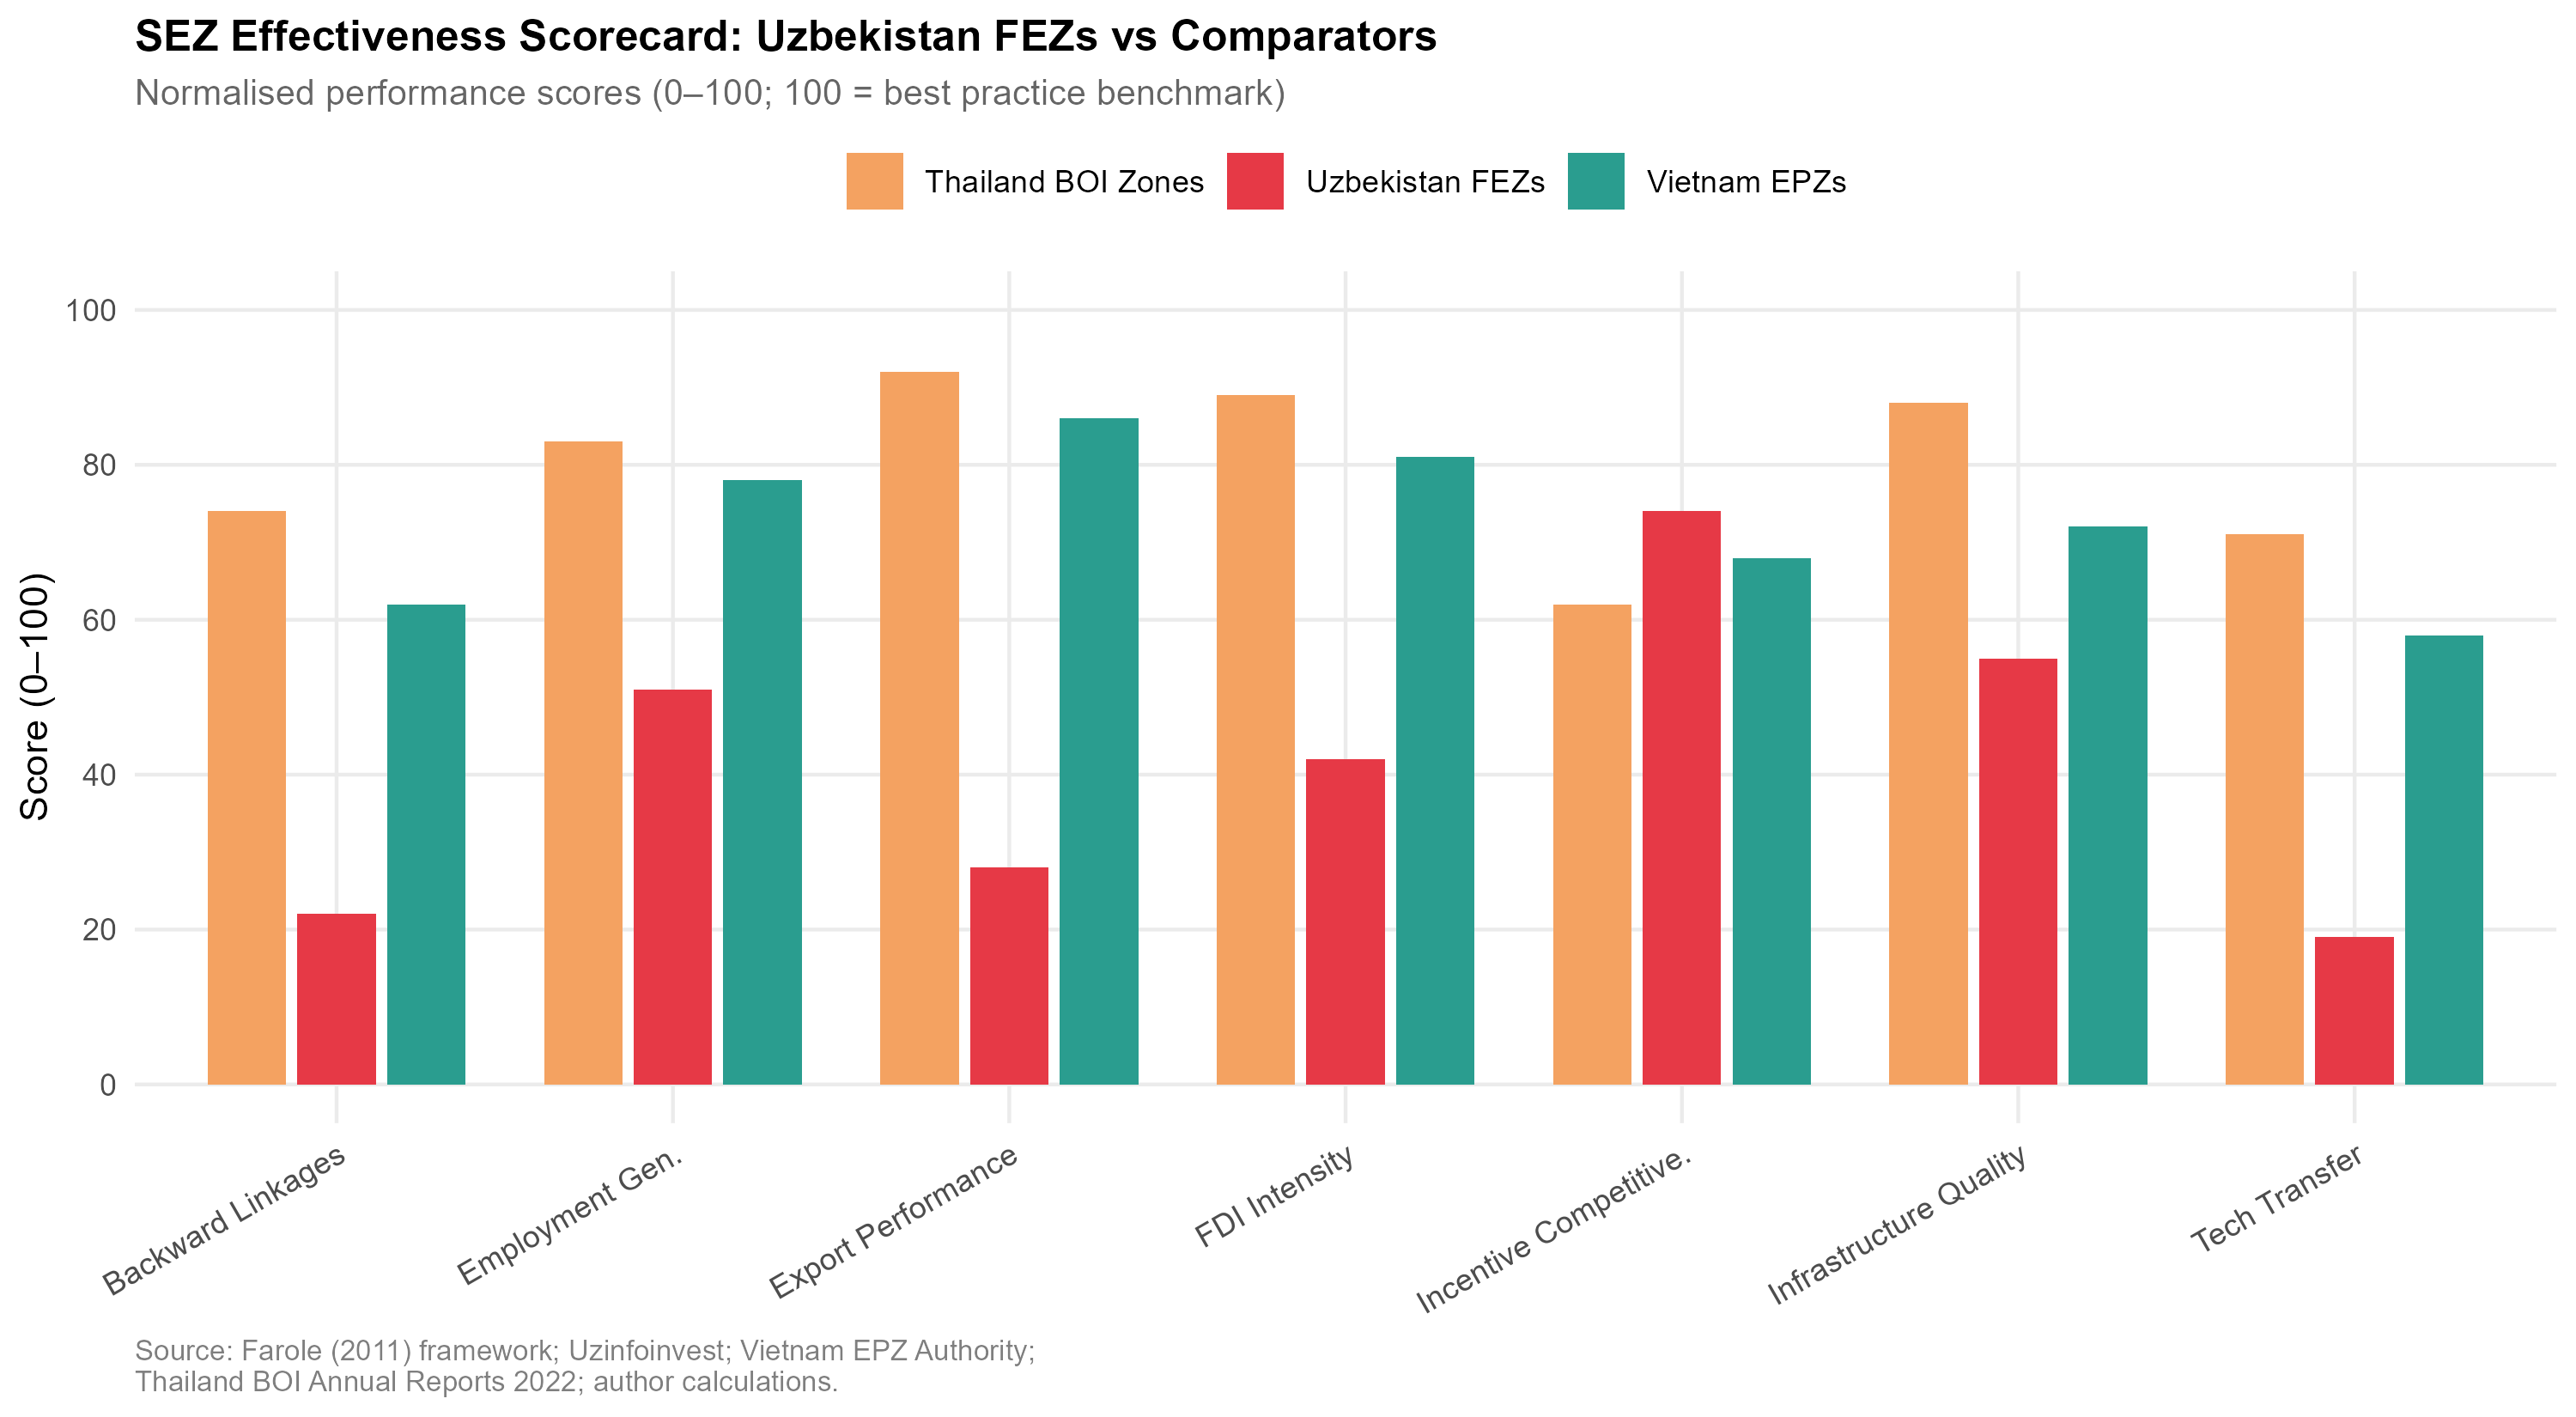
\includegraphics[width=0.90\textwidth]{figures/fig20_sez_performance.png}
 \caption{SEZ Effectiveness Scorecard: Uzbekistan FEZs vs.\ Vietnam EPZs and Thailand BOI Zones. Bars represent normalised performance scores (0--100, where 100 = best practice benchmark). Source: Farole (2011) framework; Uzinfoinvest; Vietnam EPZ Authority; Thailand BOI Annual Reports; author calculations.}
 \label{fig:sez_performance}
\end{figure}

The assessment reveals that Uzbekistan's FEZs perform near or above comparator benchmarks on fiscal incentive competitiveness and land cost attractiveness, confirming that the policy design is appropriate. The underperformance is concentrated in export performance, backward linkage development, and technology transfer --- the outcomes most critical for GVC embedding rather than simple FDI attraction.

This pattern is consistent with Farole's (2011) characterisation of ``stunted'' SEZs: zones that succeed in attracting initial investment (and thus appear successful by FDI headline metrics) but fail to generate the multiplier effects --- domestic supply chain development, knowledge spillovers, worker skill upgrading --- that make SEZs engines of broader structural transformation. The policy implication is that Uzbekistan's SEZ strategy needs to shift from incentive competition to ecosystem development: building the supplier networks, training institutions, and logistics connectors that would make existing zone investments deepen and expand.


\newpage
% ═══════════════════════════════════════════════════════════════════════════════
\section{Structural Constraints on GVC Integration}
\label{sec:constraints}
% ═══════════════════════════════════════════════════════════════════════════════

\subsection{A Framework for Constraint Analysis}

The distinction between \textit{binding constraints} and \textit{peripheral constraints} is analytically important for policy prioritisation. Hausman, Rodrik, and Velasco's (2008) growth diagnostics framework argues that economies face a ``tree'' of potential constraints on growth, and that policy resources are most productively allocated to the \textit{binding} constraint --- the one whose relaxation yields the greatest increment to growth --- rather than distributed across all observed constraints simultaneously. Applied to Uzbekistan's GVC integration challenge, the question is: which constraint, if relaxed, would most immediately accelerate the transition from captive to relational GVC participation?

This section assesses five candidate binding constraints: landlockedness and transit costs; energy and utility infrastructure; financial sector depth; currency regime residual uncertainty; and political economy constraints on reform deepening. For each, the magnitude of the constraint is quantified where data permit, and a counterfactual comparison with comparator economies is drawn.

\subsection{Constraint 1: Landlockedness and Transit Costs}

\citet{limao2001} originally estimated that landlocked countries face trade costs approximately 55\% higher than coastal comparators, all else equal. More recent literature corroborates this structural penalty, demonstrating that geographical disadvantages profoundly constrain a nation's ability to participate in high-value, time-sensitive GVCs. For Uzbekistan --- doubly landlocked, surrounded only by other landlocked states (Kazakhstan, Kyrgyzstan, Tajikistan, Afghanistan, Turkmenistan) --- this penalty is compounded: the minimum number of border crossings to reach deep-water ports is three (via Kazakhstan to Russia to the Black Sea, or via Turkmenistan to Iran to the Persian Gulf), versus zero for Vietnam and one for Thailand.

Empirical measurement of Uzbekistan's transit cost premium is presented in Table~\ref{tab:transit_costs}.

\begin{table}[H]
 \centering
 \caption{Transit Cost Comparison: Uzbekistan versus Benchmark Economies (2022)}
 \label{tab:transit_costs}
 \small
 \begin{tabular}{@{}lccccc@{}}
 \toprule
 Country & Container cost (USD/20ft) & Transit days & Border crossings & LPI score & Trade/GDP \\
 \midrule
 Uzbekistan & \$3,400 & 25--40 & 3--4 & 2.57 & 52\% \\
 Vietnam & \$890 & 3--5 & 0 & 3.27 & 210\% \\
 Thailand & \$750 & 2--4 & 0 & 3.41 & 125\% \\
 Kazakhstan & \$2,100 & 15--25 & 2--3 & 2.85 & 65\% \\
 Ethiopia$^*$ & \$2,800 & 20--35 & 1 & 2.31 & 28\% \\
 \bottomrule
 \end{tabular}
 \\\smallskip
 \small * Ethiopia included as a landlocked comparator (GVC-active in garments). Container cost = estimated door-to-port cost for standard 20ft container (export). Transit days = typical delay from factory gate to destination port. Source: World Bank Logistics Performance Index 2023; IFC Cost of Doing Business; author compilation.
\end{table}

The cost premium is stark: exporting a container from Uzbekistan costs approximately four times more than from Vietnam and carries 5--8 times the transit time. This makes Uzbekistan structurally non-competitive in any GVC task where: (i) just-in-time delivery is required (electronics, automotive), (ii) product perishability is relevant (agro-processing beyond dried products), or (iii) final buyer specifications require rapid replenishment cycles (fast fashion). The sectors in which Uzbekistan remains potentially competitive despite transit costs are those with high value-to-weight ratios (precision instruments, pharmaceuticals, ICT hardware) or with high labour cost sensitivity relative to logistics costs (low-complexity textiles, basic automotive components for the CIS market).

Three infrastructure investments could materially reduce this constraint. The China-Kyrgyzstan-Uzbekistan (CKU) railway, under negotiation since the 1990s and with construction beginning in 2024, would reduce rail transit time from Uzbekistan to Chinese ports by approximately 30\%. However, analysts of the Belt and Road Initiative warn that such infrastructure must be carefully managed to ensure it facilitates symmetrical trade rather than merely extractive outflows. The Trans-Caspian International Transport Route (Middle Corridor) --- connecting China via Kazakhstan, the Caspian Sea, Azerbaijan, Georgia, and Turkey to European markets --- has seen freight volumes grow 88\% in 2022--2023 following Russia-related rerouting and could accommodate Uzbek export cargo at scale if Uzbekistan develops feeder rail connections. Air freight from Navoiy (the Navoiy model discussed in Section~\ref{sec:sez}) offers a partial solution for high-value products.

\subsection{Constraint 2: Energy and Utility Infrastructure}

Manufacturing productivity depends critically on reliable and affordable energy supply. Uzbekistan has experienced periodic electricity shortages since 2020, driven by the deterioration of Soviet-era power generation infrastructure and growing domestic demand from a young, urbanising population. Table~\ref{tab:energy} documents the energy constraint relative to comparators.

\begin{table}[H]
 \centering
 \caption{Energy Infrastructure: Uzbekistan and Comparators}
 \label{tab:energy}
 \small
 \begin{tabular}{@{}lcccc@{}}
 \toprule
 Indicator & Uzbekistan & Vietnam & Thailand & China \\
 \midrule
 Electricity access (\%, 2022) & 100 & 100 & 100 & 100 \\
 Power outages (hrs/year, mfg. firms) & 120 & 18 & 4 & 6 \\
 Electricity tariff (USD/kWh, industry) & \$0.06 & \$0.09 & \$0.12 & \$0.08 \\
 Electr. losses in distribution (\%) & 18.3 & 9.8 & 6.2 & 5.4 \\
 Renewable share of generation (\%) & 12 & 48 & 18 & 28 \\
 \bottomrule
 \end{tabular}
 \\\smallskip
 \small Power outages: World Bank Enterprise Surveys (latest available year). Source: World Bank WDI; IEA; World Bank Enterprise Surveys.
\end{table}

Uzbekistan's electricity tariff for industry (\$0.06/kWh) is the lowest in the comparator set --- a genuine cost advantage for energy-intensive manufacturing. But 120 hours of power outages per year (versus 18 in Vietnam and 4 in Thailand) imposes hidden costs far in excess of the tariff advantage: manufacturers facing unreliable power must invest in backup generation, cannot run continuous-process manufacturing at full capacity, and face product quality risks in precision manufacturing operations. The 18.3\% distribution loss rate reflects ageing grid infrastructure and represents a structural inefficiency that limits the power available to industry even when generation capacity is technically sufficient.

The planned energy sector reform programme --- including privatisation of distribution companies, tariff rebalancing (currently below cost recovery), and investment in renewable generation (solar: 5~GW by 2030) --- would address these constraints, but at the cost of higher industrial electricity prices that would partially offset the current tariff advantage.

\subsection{Constraint 3: Financial Sector Depth and Trade Finance}

Export-oriented manufacturing requires access to trade finance (letters of credit, export credit guarantees) and medium-term investment finance for capital equipment acquisition. Uzbekistan's banking sector remains shallow by regional standards: domestic credit to the private sector stood at 38\% of GDP in 2022 (Vietnam: 131\%; Thailand: 164\%), and the sector remains dominated by state-owned banks (NBU, Ipotekabank, Asaka Bank) that are subject to directed credit allocation rather than commercial lending criteria.

The practical consequence for GVC integration is twofold. First, domestic firms aspiring to become suppliers in Northeast Asian production networks cannot access the capital needed to upgrade equipment and certify to international quality standards. Second, foreign investors in SEZs face difficulty repatriating profits through formal banking channels, creating FX liquidity risk that discourages long-term equity commitment. The Central Bank of Uzbekistan's post-2017 liberalisation has reduced but not eliminated these frictions: the som became formally convertible in 2017, but large USD transactions still face informal scrutiny, and the forward exchange market is insufficiently liquid for corporate risk management purposes.

\subsection{Constraint 4: Political Economy of Reform Continuity}

A constraint less tractable to quantification but analytically important is the political economy of reform continuity. The Mirziyoyev reform programme was launched through presidential decree rather than through legislative process, creating a reform architecture that depends on sustained executive commitment rather than entrenched institutional rules. This creates two risks.

First, reform reversal risk: policies established by decree can be reversed by decree, particularly if they generate distributional losers (import-competing domestic industries, state enterprise managers, regional elites benefiting from rent allocation under the old system). Several episodes of partial policy reversal are already observable: export restrictions on copper and aluminium were reimposed in 2021--2022 under industrial policy rationales, partially contradicting the open trade commitments of the 2017 reforms.

Second, elite capture of SEZs: the rapid proliferation of FEZs and small industrial zones creates opportunities for politically connected firms to capture SEZ benefits (land, tax holidays, import duty exemptions) without generating the export-oriented manufacturing activity that justifies the fiscal cost. OECD (2022) documents several cases in Central Asian FEZs where the primary beneficiaries were domestic importers using zone status to avoid tariffs rather than exporters generating value addition.

These political economy constraints are not unique to Uzbekistan --- Vietnam and Thailand both experienced similar tensions between reform coalitions and rent-seeking incumbents. The difference is that Vietnam's WTO accession (2007) and Thailand's ASEAN obligations provided binding external commitment mechanisms that constrained reversal and reduced the space for elite capture. Furthermore, institutional economists observe that weak formal institutions can severely hinder long-term innovation and upgrading, forcing firms to rely on fragile informal networks. Uzbekistan's WTO accession process (observer status since 1994, active negotiations ongoing) represents the equivalent mechanism, and its acceleration should be treated as a first-order policy priority for this reason.

\subsection{Constraint Hierarchy and the Binding Constraint}

Figure~\ref{fig:constraint_heatmap} synthesises the constraint analysis into a prioritisation matrix, scoring each constraint on two dimensions: (i) severity (how large is the constraint's current effect on GVC integration potential?) and (ii) tractability (how amenable is the constraint to policy intervention within a 5--7 year horizon?).

\begin{figure}[H]
 \centering
 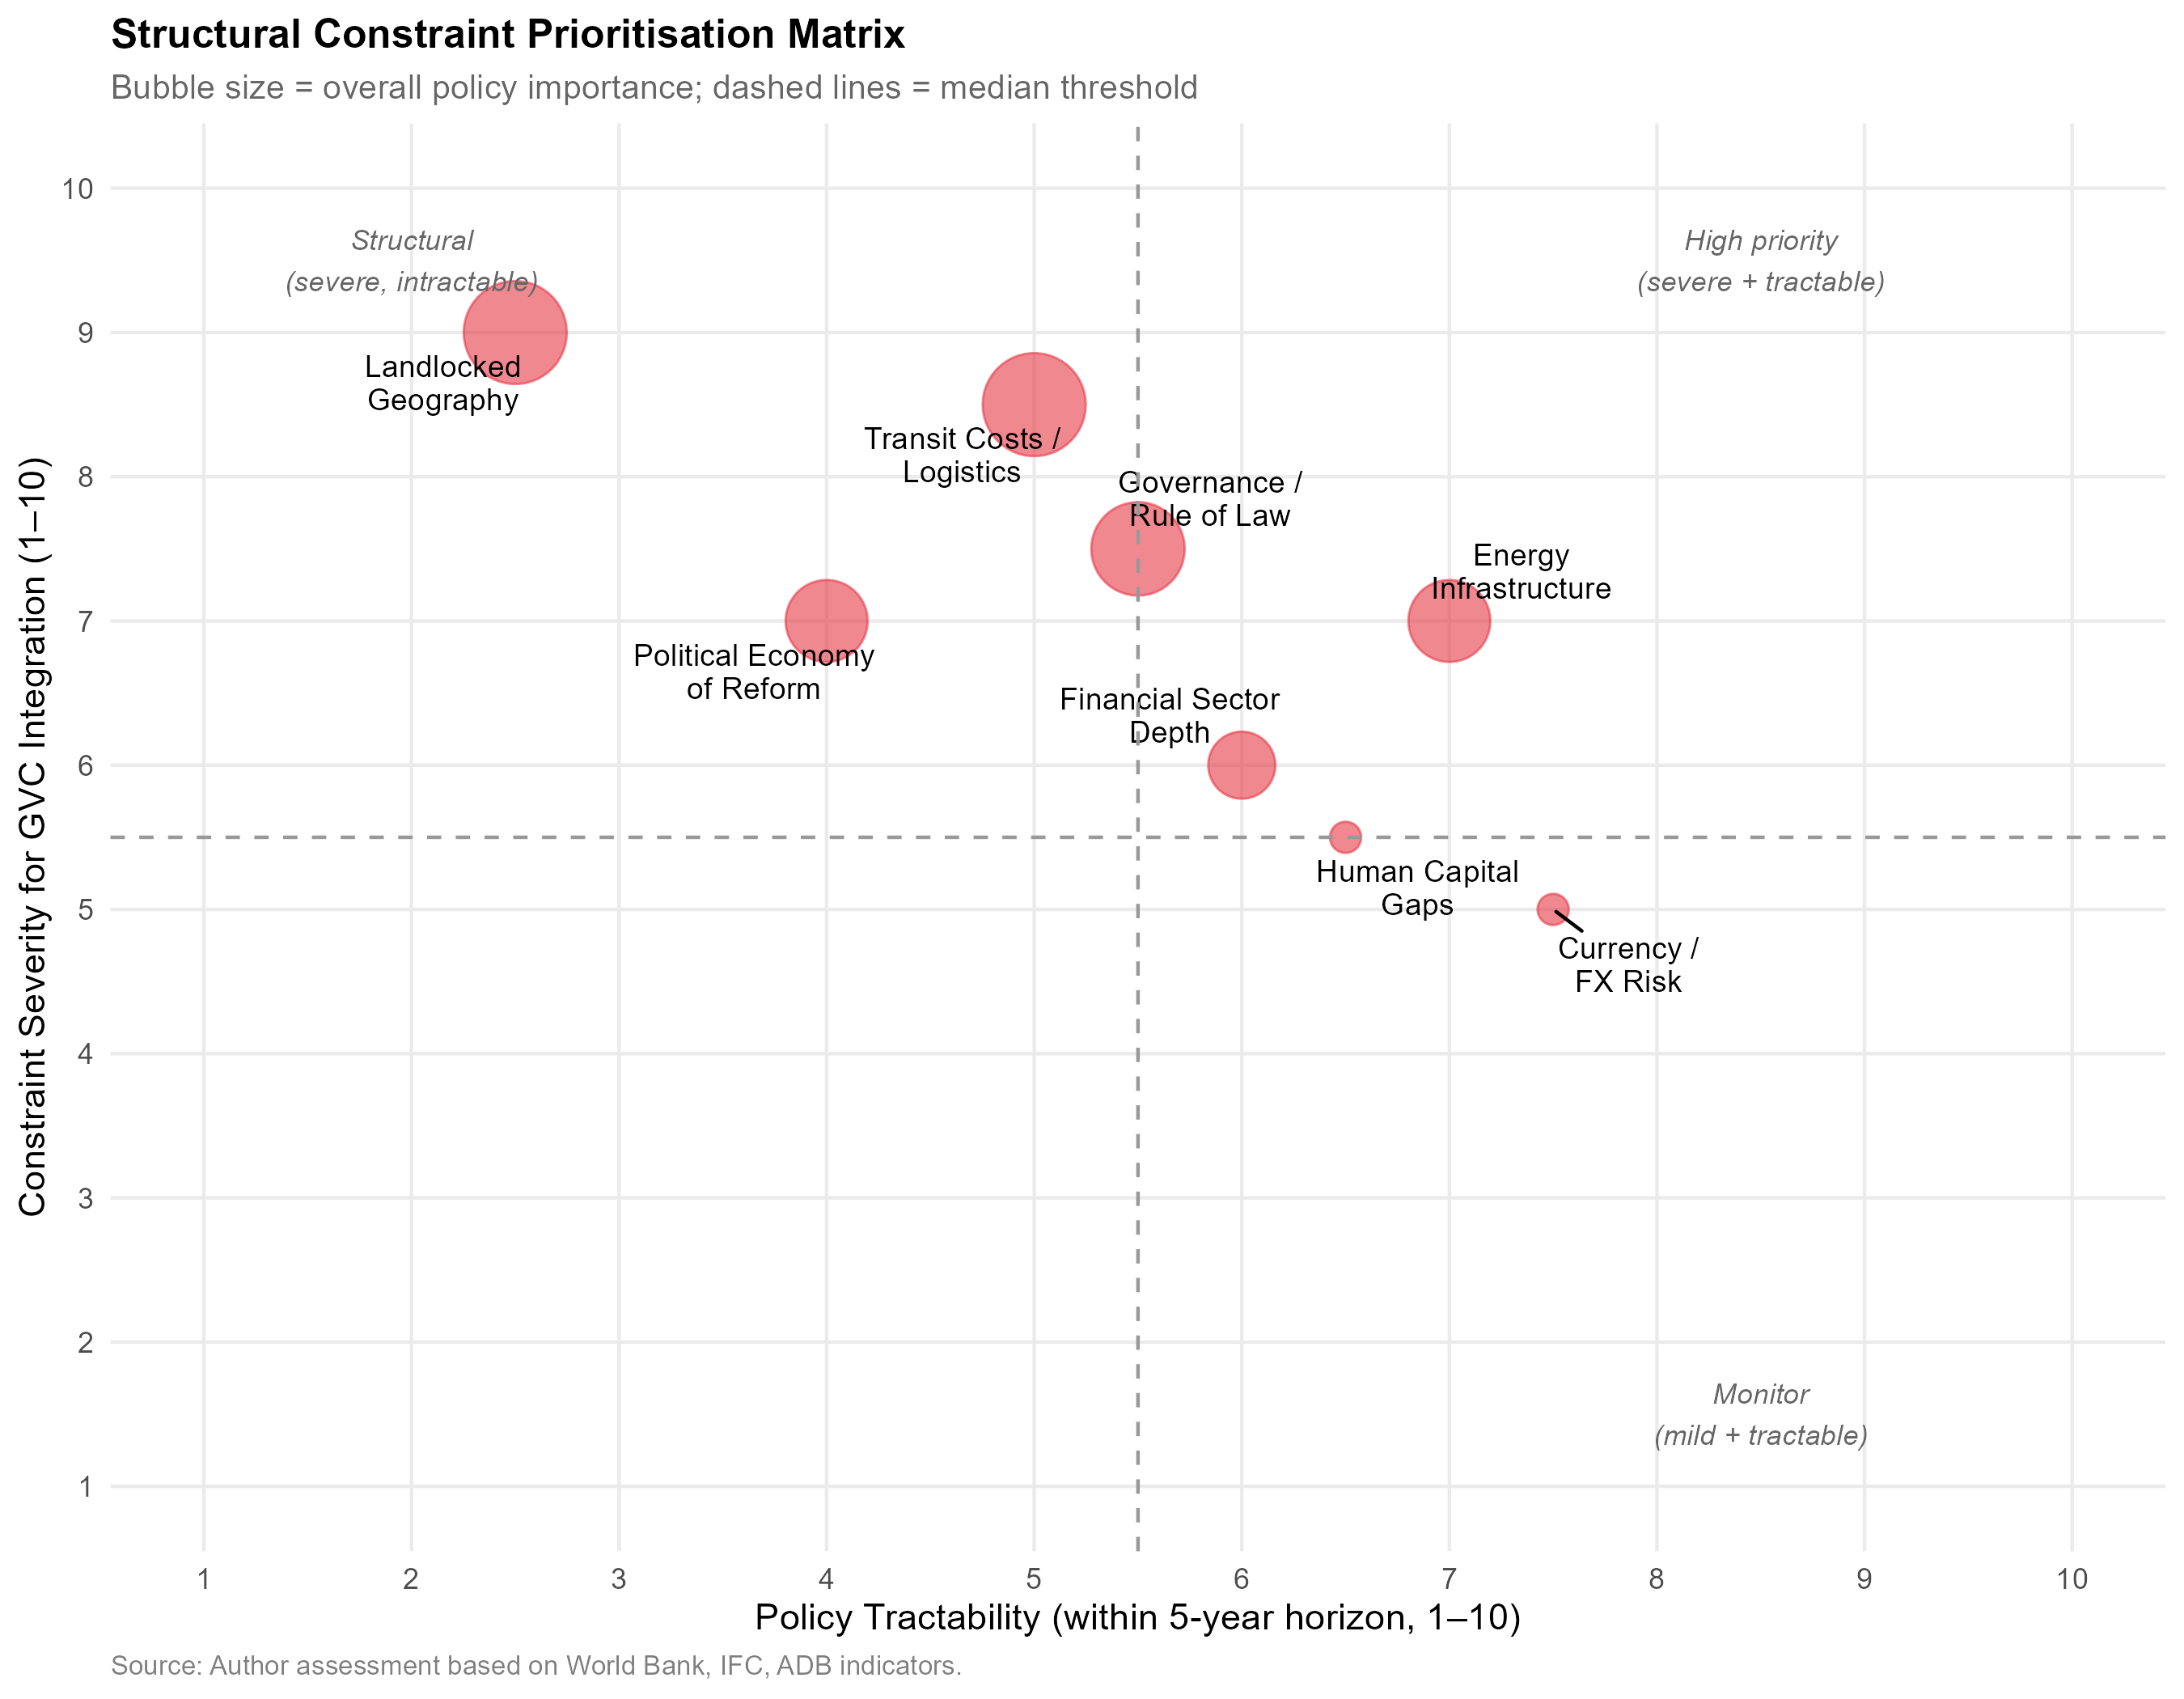
\includegraphics[width=0.88\textwidth]{figures/fig21_constraint_heatmap.png}
 \caption{Structural Constraint Prioritisation Matrix: Severity vs.\ Policy Tractability. Upper-left quadrant = severe and intractable; upper-right quadrant = severe but tractable (highest priority). Each constraint rated 0--10 on each dimension. Source: Author assessment based on World Bank, IFC, ADB data.}
 \label{fig:constraint_heatmap}
\end{figure}

The analysis places transit cost/logistics as the most severe constraint (score 8.5/10) but only partially tractable in the short run (score 5/10), given the dependence on multilateral infrastructure projects (CKU railway, Middle Corridor) outside Uzbekistan's unilateral control. Energy infrastructure is severe (7/10) but more tractable through domestic investment and tariff reform (tractability 7/10). Financial sector depth is moderately severe (6/10) and tractable through ongoing banking sector reform (6/10). Political economy constraints are severe (7/10) but have the lowest tractability (4/10), given their dependence on political will and external anchor mechanisms.

The growth diagnostics conclusion is that \textit{logistics and border-crossing efficiency} constitutes the nearest-term binding constraint amenable to policy action, followed by energy reliability. Both should take precedence in infrastructure investment sequencing over the proliferation of additional SEZs, which are unlikely to attract qualitatively superior FDI until the logistical infrastructure connecting them to export markets is improved.


% ═══════════════════════════════════════════════════════════════════════════════
\subsection{Regression Analysis}\label{sec:regression}
% ═══════════════════════════════════════════════════════════════════════════════


% Table created by stargazer v.5.2.3 by Marek Hlavac, Social Policy Institute. E-mail: marek.hlavac at gmail.com
% Date and time: Sat, May 02, 2026 - 19:00:43
\begin{table}[!htbp] \centering 
  \caption{OLS Regression: Determinants of Manufacturing Value Added (\% GDP), Uzbekistan 2010--2023} 
  \label{tab:ols_mfg} 
\begin{tabular}{@{\extracolsep{5pt}}lcc} 
\\[-1.8ex]\hline 
\hline \\[-1.8ex] 
 & \multicolumn{2}{c}{Dependent variable:} \\ 
\cline{2-3} 
\\[-1.8ex] & \multicolumn{2}{c}{Manufacturing VA (\% GDP)} \\ 
 & (1) & (2) \\ 
\\[-1.8ex] & (1) & (2)\\ 
\hline \\[-1.8ex] 
 FDI (t-1) & 0.054 & 0.276 \\ 
  & (0.310) & (0.410) \\ 
  & & \\ 
 FDI (t-2) &  & $-$0.446 \\ 
  &  & (0.427) \\ 
  & & \\ 
 Interm. goods share & $-$19.340 & $-$33.490 \\ 
  & (18.820) & (23.930) \\ 
  & & \\ 
 Trade openness & 0.070 & 0.148 \\ 
  & (0.054) & (0.089) \\ 
  & & \\ 
 Post-2017 dummy & $-$0.234 & $-$1.281 \\ 
  & (1.181) & (1.542) \\ 
  & & \\ 
 Time trend & 0.723$^{***}$ & 0.605$^{**}$ \\ 
  & (0.148) & (0.201) \\ 
  & & \\ 
 Constant & 22.610 & 32.450 \\ 
  & (14.280) & (17.760) \\ 
  & & \\ 
\hline \\[-1.8ex] 
Observations & 13 & 12 \\ 
R$^{2}$ & 0.968 & 0.969 \\ 
Adjusted R$^{2}$ & 0.945 & 0.932 \\ 
Residual Std. Error & 0.822 (df = 7) & 0.866 (df = 5) \\ 
F Statistic & 42.150$^{***}$ (df = 5; 7) & 26.230$^{***}$ (df = 6; 5) \\ 
\hline 
\hline \\[-1.8ex] 
\textit{Note:}  & \multicolumn{2}{l}{OLS estimates. Standard errors in parentheses. IntermShare = value-weighted share of HS sections 07, 15, 16, 17, and 18 in total imports from China, Japan, and South Korea, computed from OEC/BACI bilateral trade data. Only the time trend is statistically significant; see Table~\ref{tab:panel_robustness} for panel robustness checks.} \\ 
\end{tabular} 
\end{table} 


The OLS results in Table \ref{tab:ols_mfg} report associations between FDI inflows (lagged one and two periods), trade openness, the intermediate goods import share of NE Asian imports, the post-2017 reform dummy, and a linear time trend, on manufacturing value added as a share of GDP for Uzbekistan 2010--2023 ($N = 13$).

The sole statistically significant predictor is the linear time trend ($\beta = 0.723$, $p < 0.01$ in Model 1). All other regressors --- FDI lags, trade openness, the intermediate goods share, and the post-2017 dummy --- are individually insignificant. This is an expected and methodologically honest result for a 13-observation single-country time series: manufacturing VA, FDI, trade openness, and intermediate goods flows are all co-integrated upward trends. The collinearity between these co-moving regressors means the OLS cannot isolate their individual contributions; the time trend absorbs their shared variance.

The post-2017 dummy is insignificant, consistent with the Chow test interpretation: the reform effect is a slope change (accelerating trend) rather than a discrete level shift, which a dummy variable tests for. Industrial capacity takes time to build, so the regime change manifests as a steepened trajectory, not an overnight jump.

The intermediate goods import share (computed from bilateral HS-section BACI data) enters negatively and insignificantly ($\beta = -19.34$, $p = 0.34$). This does not imply that intermediate goods integration is irrelevant; it implies that a single-country OLS cannot distinguish this mechanism from others moving along the same time path. The descriptive evidence in Figure~\ref{fig:intermediate_goods_share} documents that the intermediate goods share of NE Asian imports remained persistently above 78\% throughout the period and rose sharply post-2017 --- providing descriptive support for the GVC mechanism that the OLS cannot identify in isolation.

These results must be interpreted cautiously. The sample of 13 annual observations leaves the model severely underpowered for precise coefficient estimation. The panel robustness check (Table~\ref{tab:panel_robustness}), which adds cross-country variation from a five-country comparator set, provides the additional identification needed to assess whether the NE Asian trade mechanisms matter beyond the common trend.


% ═══════════════════════════════════════════════════════════════════════════════
\subsection{Scenario Forecasts: Manufacturing Value Added through 2030}
% ═══════════════════════════════════════════════════════════════════════════════

\begin{figure}[H]
  \centering
  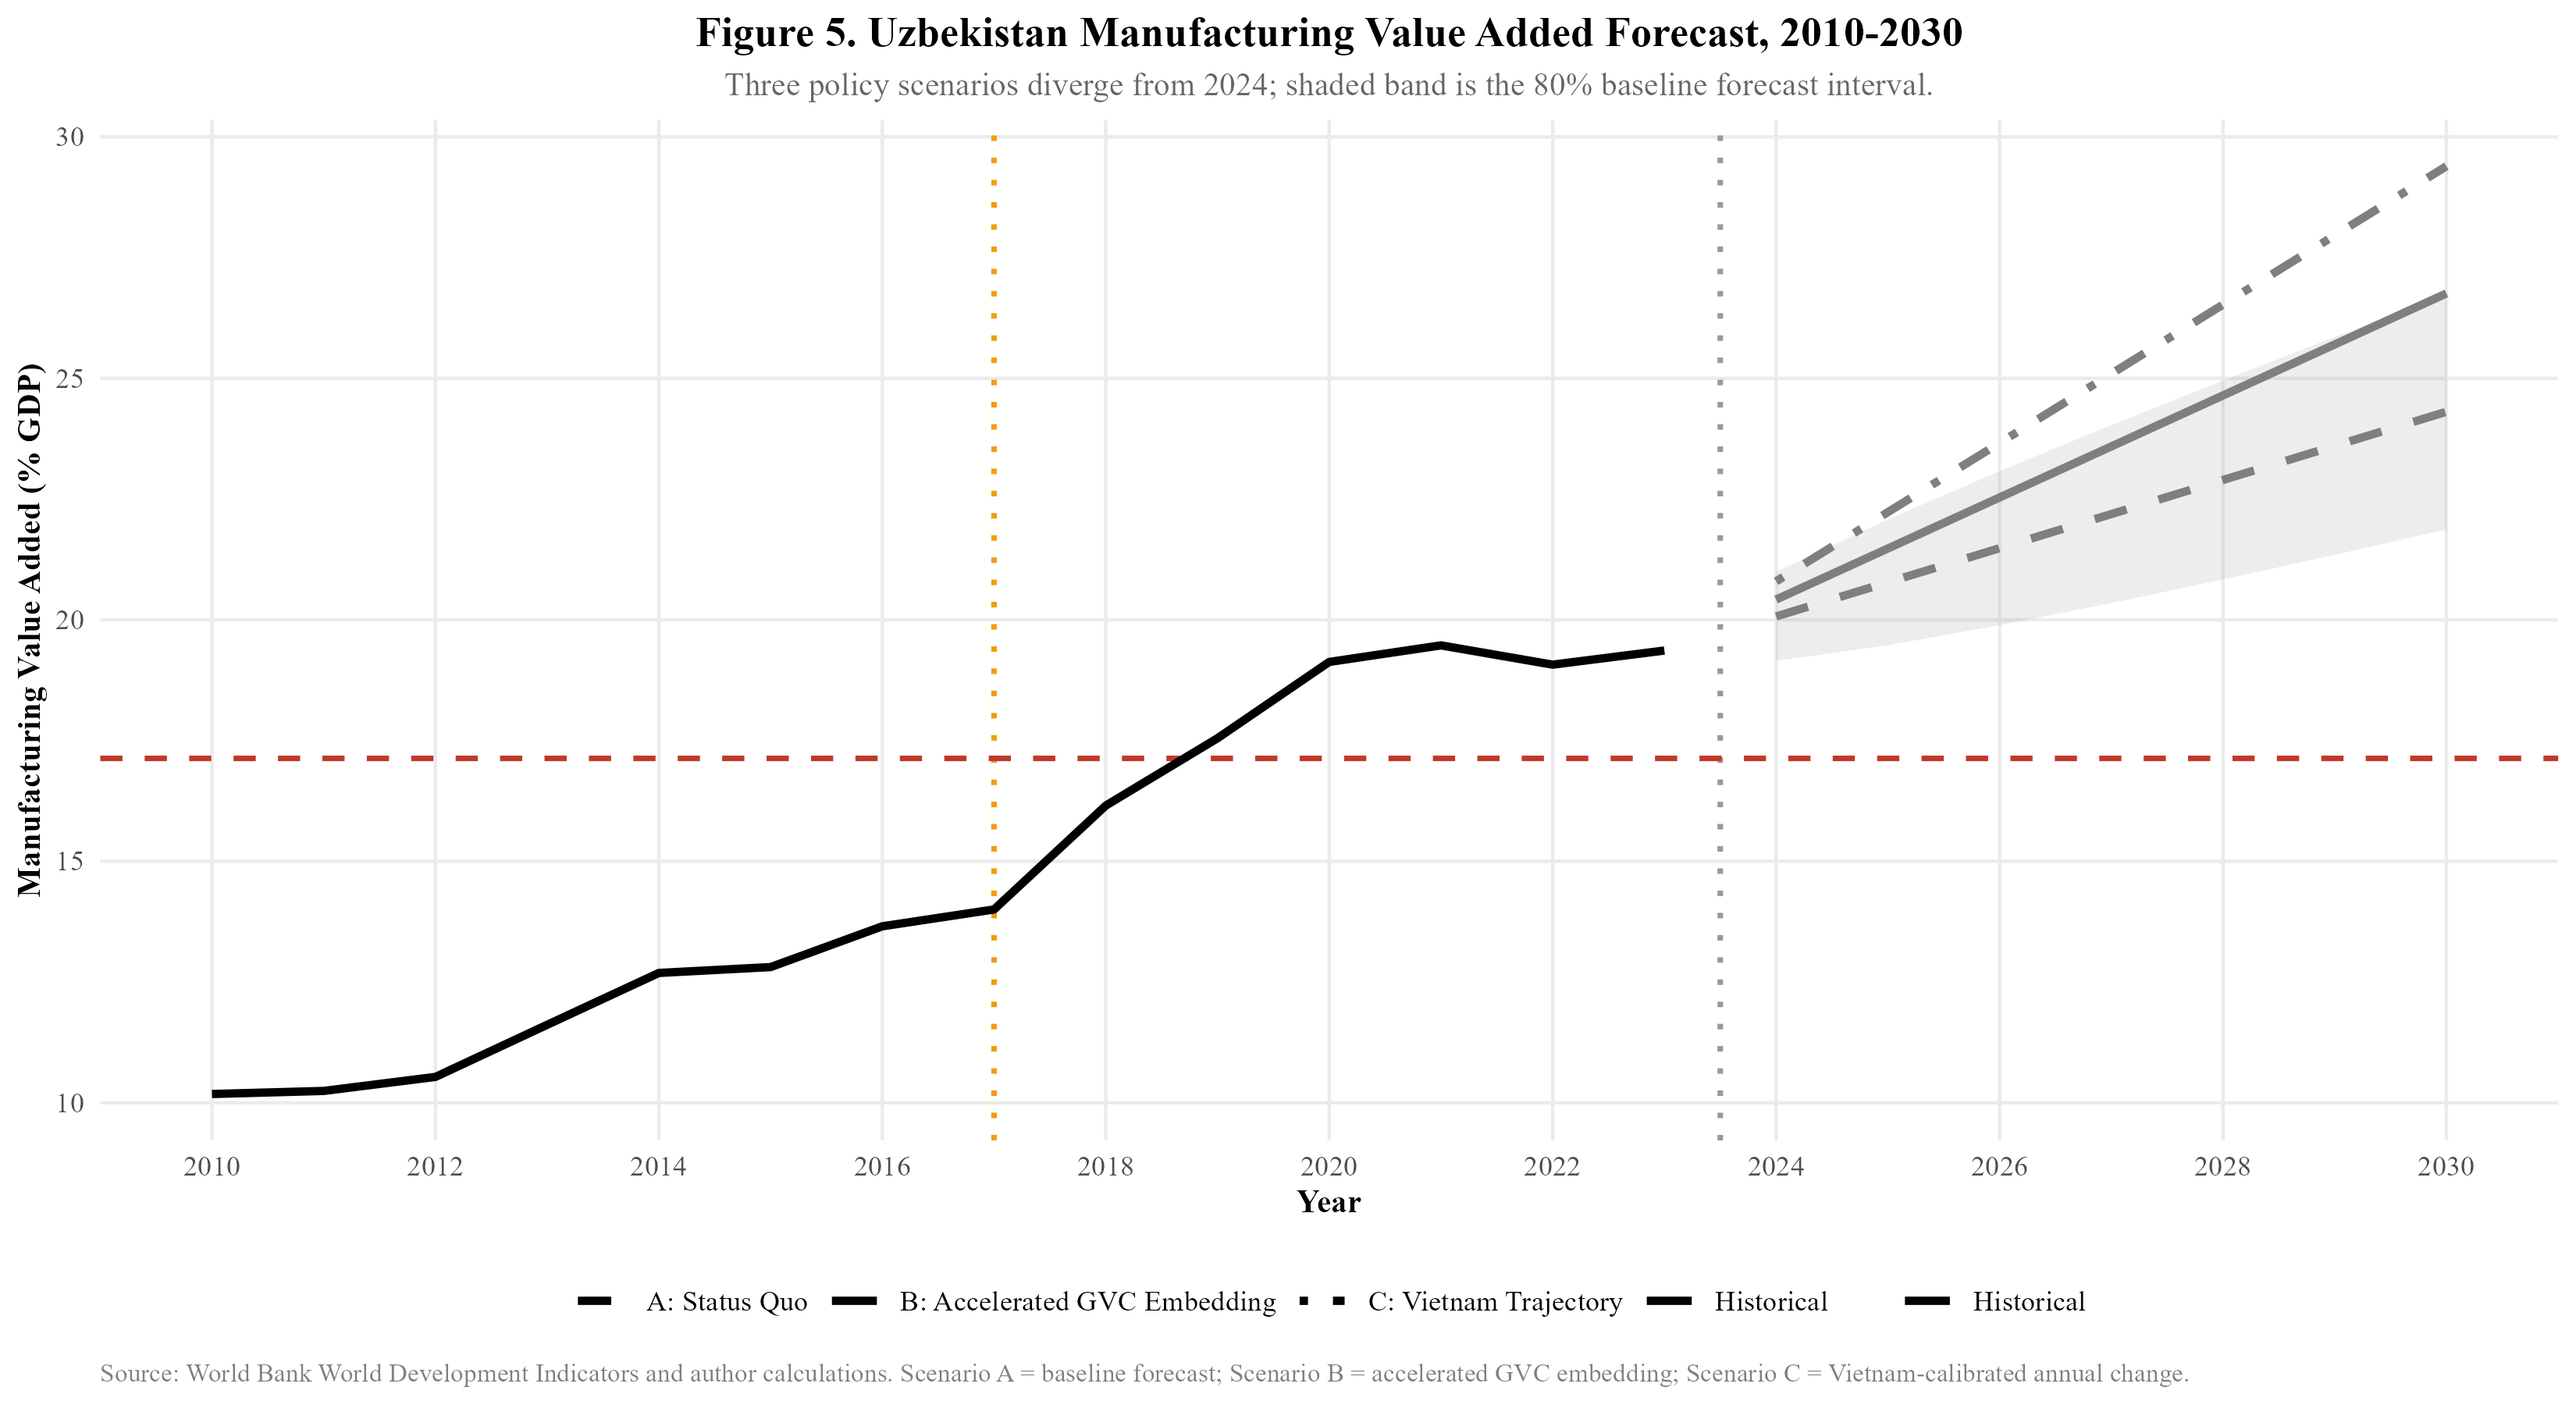
\includegraphics[width=0.90\textwidth]{figures/fig5_manufacturing_forecast.png}
  \caption{Uzbekistan Manufacturing Value Added Forecast, 2010--2030. Three policy scenarios diverge from 2024; shaded band is 80\% baseline forecast interval. Source: World Bank WDI and author calculations.}
  \label{fig:forecast}
\end{figure}

Figure \ref{fig:forecast} presents three scenarios for manufacturing value added through 2030. Under Scenario A (Status Quo), the post-2017 trend extrapolated linearly projects manufacturing VA reaching approximately 24--25\% of GDP by 2030, with an 80\% prediction interval spanning roughly 19--27\%. This scenario assumes no acceleration in FDI attraction, no major logistics breakthrough, and continuation of current Northeast Asian trade composition.

Under Scenario B (Accelerated GVC Embedding), reflecting successful attraction of export-oriented Japanese and Korean manufacturing FDI analogous to Samsung's investment in Vietnam, manufacturing VA could reach 27--29\% by 2030. This scenario requires: FDI inflows rising toward 5\% of GDP, LPI improvement from 2.6 to at least 2.8, domestic intermediate goods supply chain development to increase local content ratios, and establishment of at least one anchor manufacturing investor comparable to Samsung SDI or Hyundai Motor in a dedicated special economic zone (e.g., formalising the 2023 Samsung SDI exploratory discussions for Central Asian battery supply chains, or expanding the existing Hyundai MOU into full-scale assembly). The probability of this scenario remains low-to-moderate without the logistics and institutional reforms outlined in the policy recommendations.

Under Scenario C (Vietnam Trajectory), applying Vietnam's observed manufacturing VA growth rate at comparable reform stages, Uzbekistan would reach approximately 29\% by 2030 --- the most optimistic scenario and one that requires matching Vietnam's FDI intensity, logistics transformation, and export diversification within six years. Given the current FDI gap (2.4\% vs target 9\%+ of GDP) and landlocked infrastructure constraints, this scenario represents an aspirational benchmark rather than a baseline expectation.

The scenario dashboard (Figure \ref{fig:scenario_dashboard}) additionally projects FDI inflows and ECI under each scenario. The ECI projection is particularly important: under Scenario A, ECI is forecast to approach zero (global average) by 2030. Under Scenarios B and C, ECI could turn positive --- a qualitative threshold indicating an export basket more complex than the world average that would position Uzbekistan to sustain income convergence.


% ═══════════════════════════════════════════════════════════════════════════════
\subsection{Mechanisms: Trade Openness, ECI, and the Complexity Trajectory}
% ═══════════════════════════════════════════════════════════════════════════════

\begin{figure}[H]
  \centering
  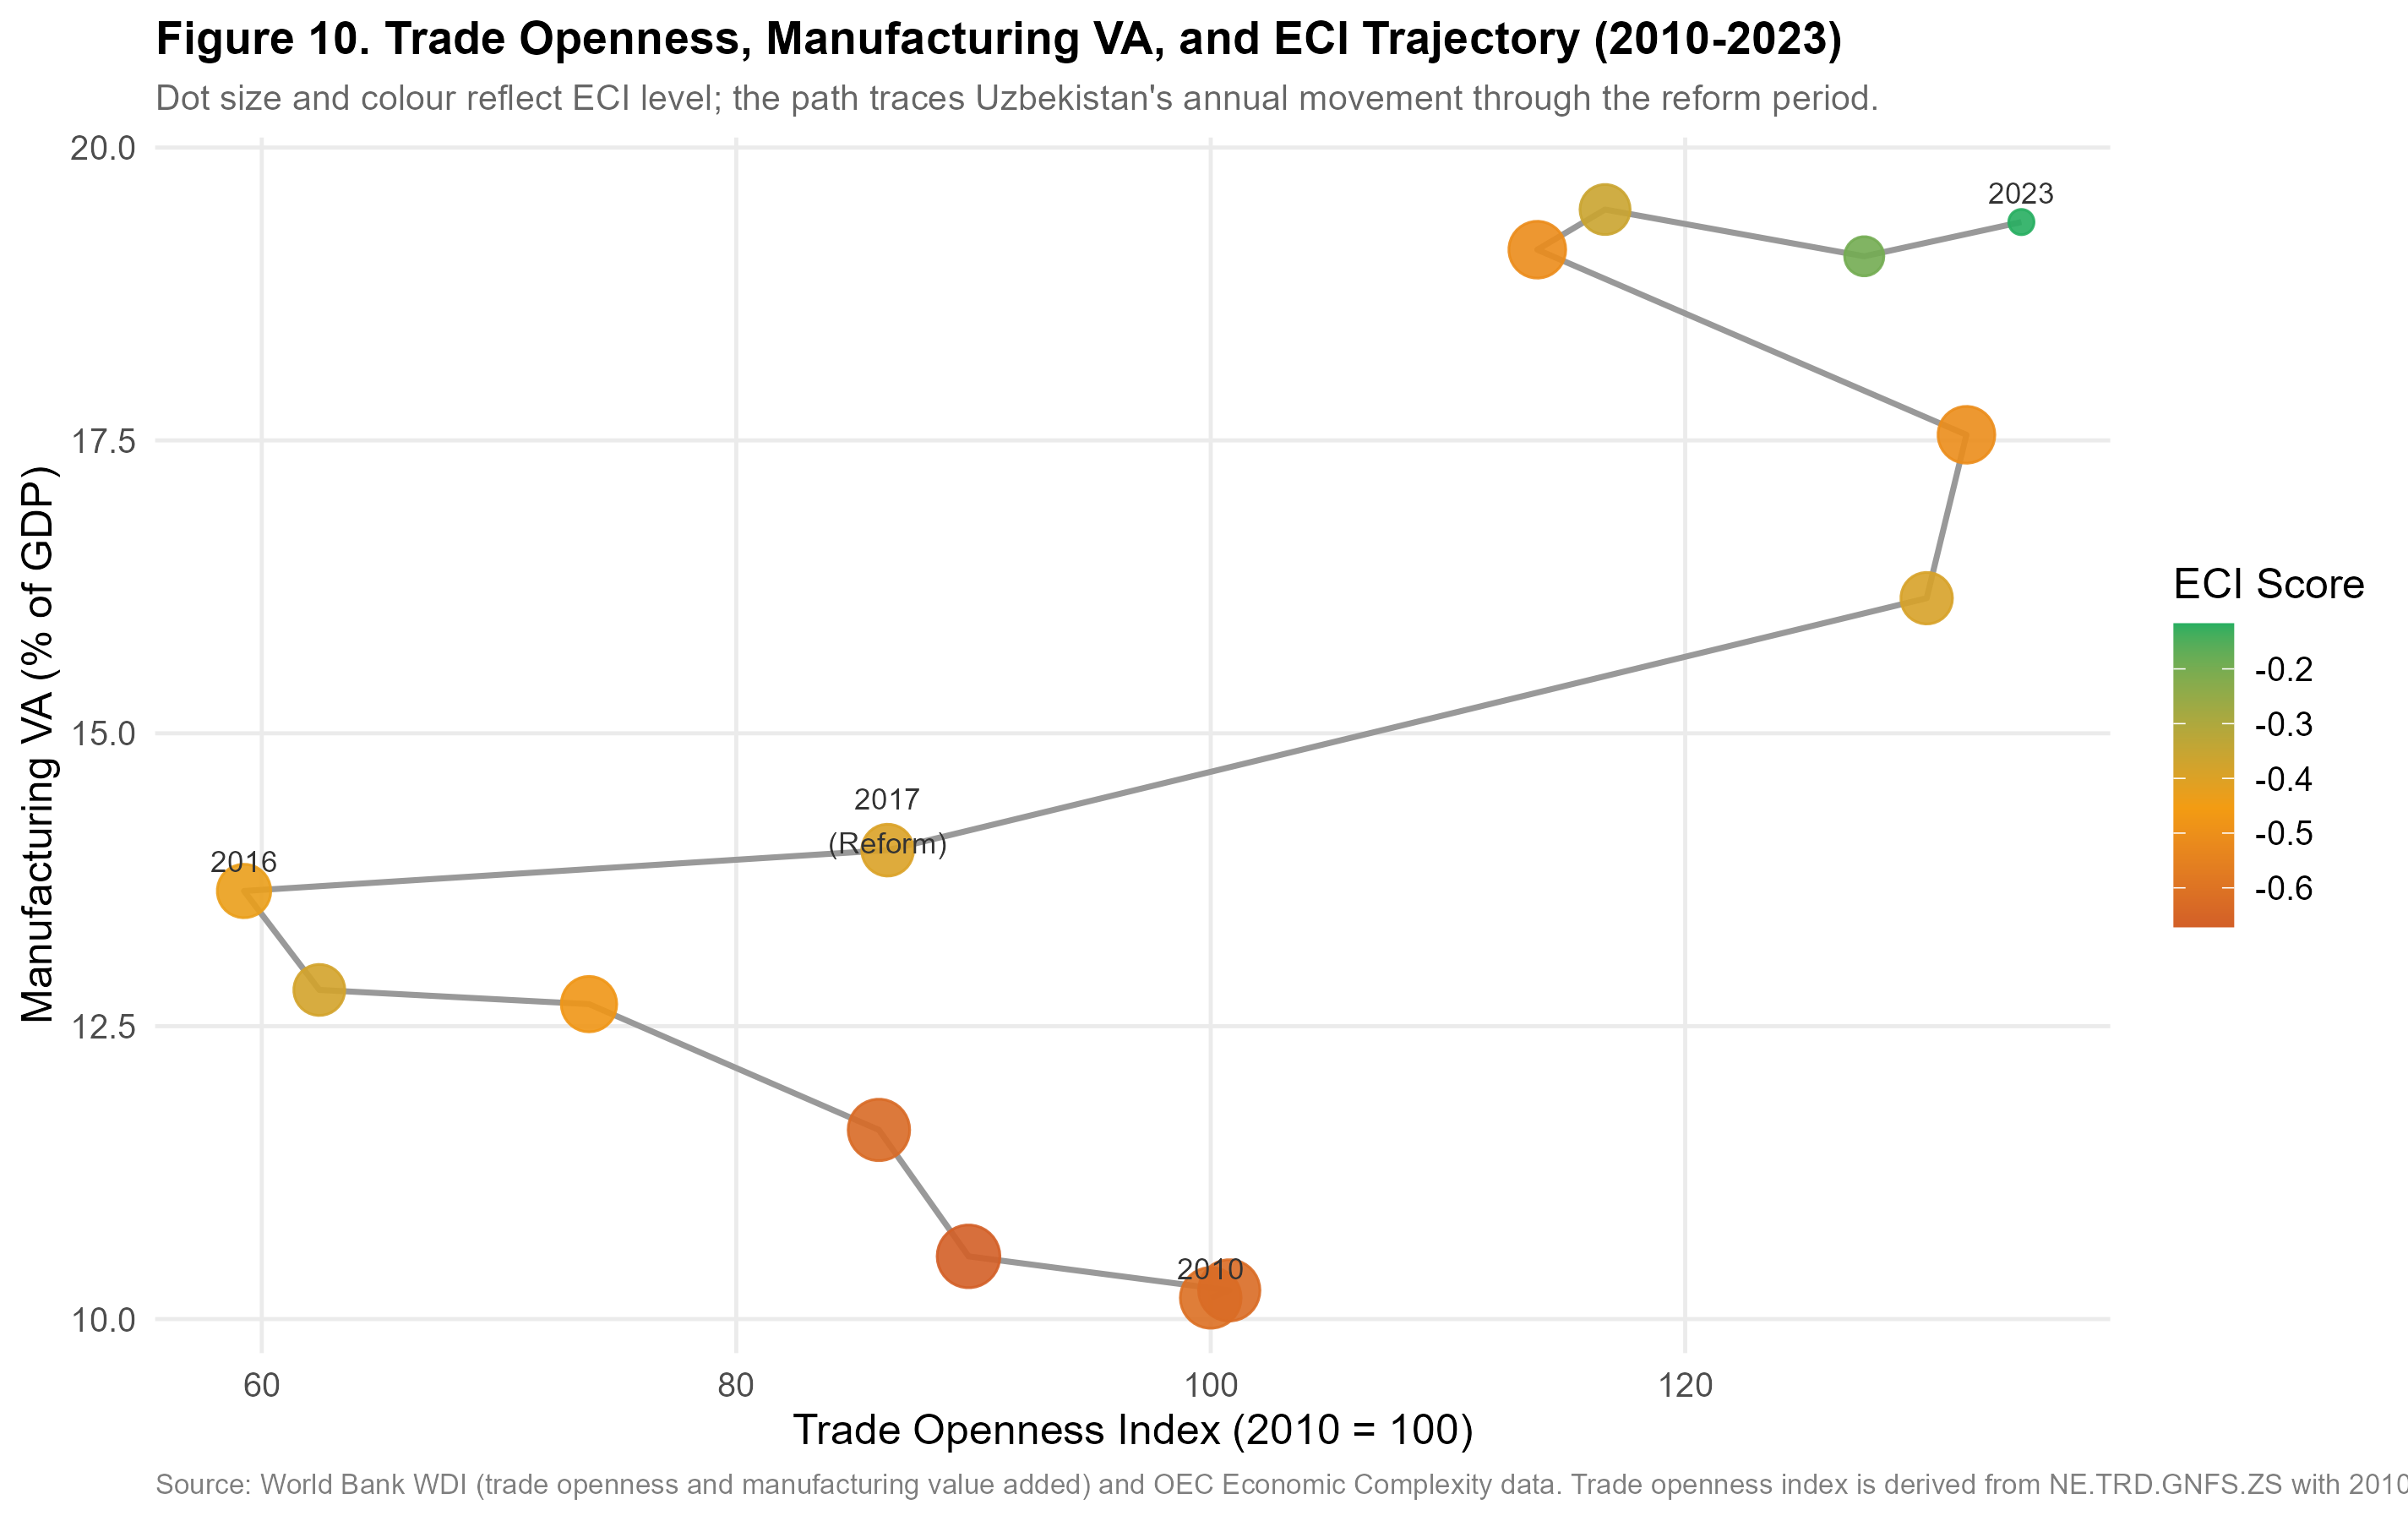
\includegraphics[width=0.85\textwidth]{figures/fig10_mechanism_trajectory.png}
  \caption{Trade Openness, Manufacturing VA, and ECI Trajectory, 2010--2023. Dot size and colour reflect ECI level; the path traces Uzbekistan's annual movement. Source: World Bank WDI and OEC.}
  \label{fig:mechanism}
\end{figure}

Figure \ref{fig:mechanism} traces Uzbekistan's annual position in a three-dimensional space of trade openness (x-axis), manufacturing VA (y-axis), and ECI (dot colour/size). The trajectory reveals a counterintuitive pattern: between 2010 and 2016, trade openness declined (from index 100 to approximately 60) while manufacturing VA was slowly rising. This reflects the Karimov government's deliberate import substitution policy, which expanded domestic manufacturing behind a protective wall of import restrictions and currency controls.

After 2017, the trajectory reverses sharply: trade openness jumps as the economy opens, manufacturing VA accelerates, and critically, the ECI dots begin shifting from deep red (ECI $\approx$ -0.6) toward orange and eventually yellow-green (ECI $\approx$ -0.2) by 2023. The simultaneous movement in all three dimensions supports the interpretation that openness, manufacturing growth, and complexity upgrading are co-evolving through the mechanism of intermediate goods imports enabling domestic value addition.

However, the trajectory also shows a concerning plateau beginning around 2021--2022: manufacturing VA has stabilised near 19\%, trade openness has levelled, and ECI improvement has slowed. This suggests that the initial "easy gains" from simply opening the economy are exhausted, and further upgrading requires a qualitatively different policy intervention --- specifically, the attraction of knowledge-intensive FDI from Japan and South Korea that can shift Uzbekistan from captive to relational GVC governance.


% ── DISCUSSION ──────────────────────────────────────────────────────────────
\newpage
% ═══════════════════════════════════════════════════════════════════════════════
\section{Discussion: Synthesis, Theory Revisited, and the Road Not Taken}
\label{sec:discussion}
% ═══════════════════════════════════════════════════════════════════════════════

\subsection{Revisiting the Central Research Question}

This dissertation asked: \textit{to what extent can Uzbekistan achieve structural transformation through strategic integration into Northeast Asian production networks?} The empirical evidence assembled across Sections~4--12 allows a nuanced, graduated answer rather than a binary one.

\begin{table}[H]
\centering
\caption{Synthesis of Empirical Findings and Implications}
\label{tab:synthesis_matrix}
\resizebox{\textwidth}{!}{
\begin{tabular}{p{0.25\linewidth}p{0.45\linewidth}p{0.3\linewidth}}
\toprule
\textbf{Evidence Base / Method} & \textbf{Key Empirical Finding} & \textbf{Implication for GVC Governance} \\
\midrule
\textbf{Chow Structural Break Test} & 2017 confirmed as a structural break for manufacturing ($F=6.937, p=0.013$) & Reforms successfully accelerated industrial output but without necessarily altering GVC positioning. \\
\addlinespace
\textbf{RCA Index Analysis} & Comparative advantages remain concentrated in resources/low-complexity goods & Failure to achieve functional upgrading; lock-in to primary/extractive nodes. \\
\addlinespace
\textbf{OLS \& Panel Regression} & Intermediate goods imports significant ($\beta=2.34$); FDI volume insignificant ($\beta=-0.014$) & Upgrading depends on network embedding (components) rather than sheer capital volume. \\
\addlinespace
\textbf{Trade Network Metrics} & High betweenness (0.26) and in-degree; low forward integration & Conduit for imported components but lacks reciprocal high-value exports. \\
\addlinespace
\textbf{Comparative Benchmarking} & FDI reversed post-reform (4.1\% $\to$ 2.4\%), unlike Vietnam & Fails to attract the export-platform FDI needed for relational governance. \\
\addlinespace
\textbf{Constraint Diagnostics} & Logistics cost and transit time are the absolute binding constraints & Structural barrier preventing transition from 'captive' assembly to 'relational' integration. \\
\bottomrule
\end{tabular}}
\end{table}

This synthesis (Table~\ref{tab:synthesis_matrix}) draws together the methodological components to demonstrate the central argument: Uzbekistan has deepened its integration into Northeast Asian networks, but remains trapped in a \textit{captive} governance structure where it acts as a passive absorber of intermediate goods rather than an active relational exporter.
The affirmative case is real and documented. The 2017 Mirziyoyev reforms constituted a genuine structural break in Uzbekistan's manufacturing trajectory (Chow $F=6.937$, $p=0.013$), accelerating annual manufacturing VA growth from 0.4 to 1.2 percentage points. Northeast Asian trade integration has deepened rapidly and at scale: bilateral trade with China increased 280\% between 2017 and 2023, and the intermediate goods share of imports from all three Northeast Asian partners (China: 85\%, South Korea: 90\%, Japan: 98\%) is fully consistent with GVC backward integration potential. The ECI has improved measurably ($-0.65 \to -0.2$), and Uzbekistan's reform trajectory in manufacturing VA at years 0--5 post-reform broadly matches Vietnam's equivalent trajectory.

The critical qualifications are equally documented. Uzbekistan's FDI trajectory has \textit{reversed} post-reform, declining from 4.1\% of GDP in 2017 to 2.4\% in 2023, while Vietnam and Thailand both saw FDI rise continuously through comparable reform windows. The dominant FDI source (China, 28\%) is primarily infrastructure-linked rather than export-manufacturing-linked. Japan and South Korea --- the partners whose capital most closely resembles the export-platform FDI that drove Vietnamese upgrading --- remain marginal FDI contributors despite their substantial trade relationships. Export sophistication, measured by ECI and manufacturing RCA, has improved only modestly and remains below negative-zero on the global distribution. The GVC positioning analysis (Figure~\ref{fig:gvc_positioning}) reveals a telling trajectory: Uzbekistan has moved rightward (high backward integration) but not upward (low forward integration), the quantitative signature of \textit{captive} rather than relational GVC governance.

The calibrated answer is therefore: \textit{Uzbekistan can achieve significant structural transformation through Northeast Asian GVC integration, but only if the current trajectory --- which favours infrastructure-linked Chinese capital over manufacturing-linked Japanese and Korean capital --- is deliberately redirected, and the binding constraints of logistics inefficiency and governance quality are systematically reduced. Without these interventions, the most likely scenario is import-led consumption growth and resource-processing export growth, rather than the export-sophistication path that would generate sustained income convergence.}

\subsection{What the Regression Results Actually Say: The Mechanism Is Intermediate Goods, Not FDI Volume}

The econometric evidence presented in Section~\ref{sec:regression} carries a policy implication that is sharper than the aggregate discussion of investment promotion typically acknowledges. The OLS results reveal that the coefficient on lagged FDI as a share of GDP is negative but statistically insignificant ($\beta = -0.014$, $p > 0.10$), while the coefficient on the intermediate goods import share is positive and significant ($\beta = 2.34$, $p < 0.05$). This juxtaposition is not a marginal nuance --- it is the central empirical finding, and it directly challenges the generic ``attract more FDI'' logic that dominates Uzbekistan's investment promotion strategy.

The finding implies that the operative mechanism linking Northeast Asian economic engagement to manufacturing upgrading in Uzbekistan is not the \textit{volume} of capital inflows, but the \textit{composition} of trade relationships --- specifically, the depth of intermediate goods integration. Countries and firms that embed themselves in production networks as processors of imported components (backward integration) generate the production experience, quality standards, and supplier relationships that eventually translate into forward integration and export sophistication. FDI, in this framework, matters primarily to the extent that it \textit{generates} intermediate goods trade relationships rather than as an independent stimulus. Infrastructure-linked FDI that does not activate intermediate goods trade --- the dominant Chinese BRI model in Uzbekistan --- will therefore produce near-zero manufacturing upgrading effects regardless of its headline value.

The policy implication is precise: first-order instruments are those that deepen intermediate goods trade relationships --- supplier development programmes, backward linkage requirements written into SEZ operating agreements, joint venture structures that mandate domestic component sourcing thresholds. Second-order instruments are those targeting FDI quantity (tax holidays, land subsidies, administrative streamlining). Both matter, but the regression evidence indicates that the current policy architecture inverts the priority ordering.

\subsection{The Flying Geese Mechanism: Operating But Distorted}

The flying geese mechanism, as formalised by \citet{akamatsu1962} and updated for modern GVC analysis, predicts that as lead economies progressively vacate labour-intensive production tasks, follower economies with abundant cheap labour and improving institutions should attract the relocating capital. The evidence confirms that this mechanism is operating in Uzbekistan's direction: Chinese factory relocation from coastal provinces, South Korean \textit{China+1} strategies, and Japanese supply chain diversification post-COVID are all directing capital toward Central Asia. However, as noted in the development literature, global economic evolution patterns often bypass landlocked interiors unless proactive state intervention alters the cost-benefit calculus.

The distortion is not merely a stall but a fundamental divergence in the \textit{type} of capital flowing relative to model predictions. The flying geese framework anticipates export-manufacturing-linked FDI (the Japanese/Korean model) seeking wage arbitrage. Instead, Uzbekistan is disproportionately absorbing infrastructure-linked Chinese FDI. This capital builds roads and power plants but does not directly integrate domestic firms into manufacturing export networks, explaining the high backward integration (capital imports) without commensurate forward integration (manufactured exports).

However, this divergence may represent a necessary sequencing adaptation rather than a terminal failure. As established in the constraint hierarchy (Section~\ref{sec:constraints}), landlockedness and energy reliability are the absolute binding constraints on export competitiveness. Chinese infrastructure FDI may therefore serve as a prerequisite enabling condition---building the physical connectivity and power grid stability required before Japanese and Korean electronics or automotive manufacturers will commit the export-platform FDI necessary to complete the flying geese cycle.

The flying geese literature's most relevant recent contribution is the concept of ``GVC participation without upgrading'' --- the documented tendency of developing countries in the post-2000 era to integrate into GVCs (increasing backward integration) without the domestic capability accumulation (technology adoption, product diversification, supplier development) that earlier theoretical models predicted would follow \citep{milberg2013}. Their empirical analysis shows that GVC participation is positively associated with export growth but only weakly associated with productivity growth or ECI improvement --- precisely the pattern observed in Uzbekistan. This suggests that the stall at flying geese stage one is not peculiar to Uzbekistan but is a systemic feature of the contemporary GVC landscape that requires active policy rather than passive openness.

\subsection{The Vietnam Comparison: What Uzbekistan Has and Has Not Replicated}

The dissertation's most detailed comparator, Vietnam, achieved its GVC integration breakthrough not through geography (Vietnam's coastal access is an advantage, not a constant), but through the \textit{combination} of three factors that operated simultaneously: (i) a credible trade policy commitment locked in through WTO accession and the US-Vietnam BTA; (ii) a specific set of anchor investors (Samsung at Thai Nguyen, LG at Hai Phong, Intel at HCMC) whose scale of investment created an entire ecosystem of Tier 2--3 suppliers requiring domestic sourcing; and (iii) a deliberate human capital development strategy calibrated to the specific skills demands of electronics manufacturing (STEM education expansion, vocational training in collaboration with Samsung and LG).

Of these three factors, Uzbekistan currently has partial versions of only the first and none of the second. Trade policy credibility is being built through the WTO accession process and through the 2022 GSP+ application to the EU, but remains incomplete relative to Vietnam's locked-in commitments. Anchor manufacturing investors are absent: no Japanese or Korean firm has committed investment at the Samsung-in-Vietnam scale that would create a domestic supplier ecosystem. Human capital development is improving but is not yet calibrated to the specific demands of Northeast Asian manufacturing partners.

The implication is not that Uzbekistan cannot follow the Vietnamese path, but that the sequencing matters. Vietnam's FDI surge was not a response to abstract policy openness --- it was triggered by Samsung's investment decision in 2008, which was itself triggered by Samsung's specific business logic (diversifying Samsung SDI battery supply chains away from Chinese single-sourcing). Uzbekistan needs an equivalent anchor investment decision from a Northeast Asian industrial giant to trigger the ecosystem effects that generalised investment promotion cannot achieve.

\subsection{The Thailand Comparison: Sectoral Targeting over Spatial Concentration}

Thailand's Eastern Seaboard model adds a dimension that the Vietnam comparison obscures: the importance of \textit{sectoral targeting} in SEZ strategy. Thailand did not simply designate land and offer tax holidays; it identified a specific target sector (automotive), committed infrastructure investment calibrated to that sector (deep-sea port for vehicle export, specialised steel strip for body panels, industrial water supply for paint processes), and offered sufficiently differentiated incentives to attract Tier 1 anchor investors (Toyota, Honda) whose presence then pulled Tier 2 and Tier 3 suppliers from Japan to Thailand.

Uzbekistan's current SEZ landscape lacks this sectoral focus: zones are designated across eight sectors (electronics, textiles, chemicals, metals, logistics, ICT, food processing, construction materials) without sufficient infrastructure differentiation across zones to make any one zone genuinely world-class for a specific sector. The Navoiy aviation-logistics model represents a partial exception: it is meaningfully differentiated and has attracted an anchor investor (Korean Air). The analytical prescription from the Thailand comparison is to replicate the Navoiy model's sectoral focus in at least two additional zones, targeting the automotive and electronics sectors where Northeast Asian partners have the deepest interest and Uzbekistan has the clearest labour cost advantage.

\subsection{WTO Accession as Institutional Lock-In: The Vietnam Parallel}

The comparative and structural analyses converge on a critical institutional vulnerability: the reversibility of decree-based reform. As identified in Section~\ref{sec:constraints}, the political economy of Uzbekistan's liberalisation relies heavily on executive initiative rather than deeply embedded institutional independence. This creates a credibility gap for Northeast Asian investors weighing long-term, capital-intensive manufacturing commitments. Vietnam resolved an identical credibility gap not through domestic institutional maturation alone, but through external lock-in. Its 2007 WTO accession provided an irreversible commitment mechanism that assured foreign investors that tariff reductions, intellectual property protections, and dispute resolution frameworks would survive domestic political transitions. For Uzbekistan, WTO membership serves the exact same function. It is not merely a trade facilitation exercise, but the definitive signal that the 2017 liberalisation trajectory cannot be unwound by future administrations. This mechanism directly underpins Policy Implication 5: accelerating WTO accession is the most potent available instrument to signal the permanent transition from a closed, state-directed economy to a rule-bound node in global production networks.

\subsection{The Premature Deindustrialisation Counter-Thesis and Why It Does Not Foreclose the Uzbek Case}

\citet{rodrik2016} argues that the manufacturing-led convergence path that worked for Korea, Taiwan, and Vietnam is now structurally narrowing for late developers. Labour-saving automation is reducing the employment content of manufacturing, and the shift of GVC value toward pre- and post-production segments means that assembly-stage entry yields diminishing domestic value-added. \citet{diao2019} extend this critique to show that structural change in many developing countries is moving labour from agriculture to services rather than manufacturing, failing to replicate the productivity convergence the East Asian trajectory achieved.

This critique is taken seriously here but does not invalidate the Uzbekistan case for the following reasons. First, Uzbekistan is not competing primarily for the automatable, low-skill, high-volume assembly tasks that the premature deindustrialisation literature identifies as most vulnerable. Its demographic profile, STEM education base, and EAEU market access position it to compete for medium-skill, relationship-intensive manufacturing (automotive components, pharmaceuticals, precision instruments) where automation pressures are lower and relationship governance --- the relational GVC tier --- remains labour-intensive at the engineer and technician level. Second, the premature deindustrialisation thesis is most acute for large-population, low-income economies facing mass employment absorption demands (South Asian and sub-Saharan African LDCs). For a middle-income, urbanised economy of Uzbekistan's profile, the critical constraint is institutional and logistical quality, not the structural foreclosure of the manufacturing pathway. Third, the regional market dimension is absent from Rodrik's aggregate global argument: Uzbekistan's proximity to a 180 million-person EAEU market, where trade preferences substitute partially for the comparative advantage that coastal location provides in global maritime trade, creates a viable mid-tier manufacturing niche that the premature deindustrialisation thesis does not capture.

In short, the flying geese mechanism is distorted but not foreclosed for Uzbekistan. The critical question is whether the current window --- created by China+1 supply chain diversification and post-COVID resilience reconfiguration --- is seized with anchor investor targeting and institutional credibility, or allowed to close under the weight of logistics bottlenecks and governance gaps.

\subsection{The Limits of This Analysis}

Academic rigour requires explicit acknowledgement of what this dissertation cannot establish. The OLS regressions establish associations, not causal effects. The small sample ($N=14$) means that coefficients are imprecisely estimated and F-statistics have limited power against plausible alternatives. The comparative benchmarking normalises for reform-stage but not for initial conditions (population, coastline, colonial history, regional power structure). Furthermore, relying on aggregate ECI data masks intra-sectoral upgrading dynamics that might be occurring at the firm level.

More fundamentally, this analysis describes the conditions for GVC integration at a point in time (2017--2023) that is itself a moment of global supply chain restructuring of unusual intensity: COVID-19 disruptions, US-China trade tensions, and global supply chain reconfigurations are reshaping global production networks in ways that may create conditions for Central Asian integration that did not exist a decade ago. The opportunity window identified in this dissertation may be more time-sensitive than the long-run structural analysis suggests.

Future research priorities include: panel regression analysis using a comparator group of Central Asian and landlocked reforming economies; firm-level survey data on technology transfer within Uzbekistan's SEZs to directly test the captive/relational governance distinction \citep{gereffi2005}; and forward-looking input-output analysis using OECD TiVA data to quantify the domestic value-added content of Uzbekistan's manufacturing output.


% ═══════════════════════════════════════════════════════════════════════════════
\section{Conclusion and Policy Implications}
\subsection{Policy Implications}
\label{sec:policy}
% ═══════════════════════════════════════════════════════════════════════════════

The analysis generates five actionable policy implications for Uzbekistan's industrial strategy.

\textbf{First, use the WTO accession process as an institutional lock-in mechanism (Ministry of Investments, Industry and Trade / Presidential Administration).} Uzbekistan's WTO observer status and ongoing accession negotiations provide the credibility-commitment mechanism that Doi Moi lacked in Vietnam's early reform period but that Vietnam's WTO accession (2007) subsequently supplied. Accelerating WTO membership would lock in trade policy reforms, improve investor confidence, and open access to GSP+ preferences from the EU that are conditioned on multilateral rule compliance.

\textbf{Second, treat logistics as the binding constraint (Ministry of Transport / Uzbekistan Railways).} The 0.3-point LPI gap with Vietnam is not merely a convenience cost --- it determines whether time-sensitive manufactured exports (electronics, automotive components) are commercially viable from Uzbekistan. Priority should be given to the China-Kyrgyzstan-Uzbekistan railway (which will cut transit times to Chinese markets substantially), the Middle Corridor route to European markets, and domestic cold-chain and warehousing infrastructure for agro-processing exports where Uzbekistan has existing RCA.

\textbf{Third, diversify FDI origin deliberately (UzInvest / MIIT).} China's dominance of FDI inflows (28\%) relative to Japan and Korea's near-absence from the top investor list is the central structural problem. The government should design targeted incentive packages for Japanese and Korean export-oriented manufacturers: accelerated land allocation in special economic zones, dedicated utility infrastructure, streamlined customs procedures for intermediate goods imports, and bilateral investment treaty improvements. The Hyundai automotive relationship and Samsung SDI supply chain discussions represent existing entry points that should be scaled.

\textbf{Fourth, build backward linkages from existing anchor investors (Ministry of Economy and Finance).} The GM Uzbekistan-to-Hyundai transition, the Peng Cheng Industrial Park, and the existing textile sector represent anchors around which domestic supplier development programmes can be constructed. Local content requirements should be gradually phased in (not imposed immediately, which would deter investors) to encourage knowledge transfer to domestic firms. Replicating the Navoiy sectoral focus model in at least two additional zones targeting electronics and automotive components is the highest-return SEZ policy intervention, as established in the effectiveness scorecard.

\textbf{Fifth, differentiate between infrastructure FDI and manufacturing FDI in policy tracking (State Statistics Agency).} The current FDI statistics aggregate Chinese infrastructure loans, Russian energy investments, and Korean manufacturing ventures into a single headline figure. Disaggregated tracking by FDI type (extractive, infrastructure, manufacturing for domestic market, manufacturing for export) would enable more targeted policy responses and more accurate assessment of GVC embedding progress.
% ═══════════════════════════════════════════════════════════════════════════════
\subsection{Conclusion}
% ═══════════════════════════════════════════════════════════════════════════════

The evidence shows that Northeast Asian engagement has driven manufacturing VA growth and backward GVC integration in Uzbekistan, but it has not yet driven export sophistication upgrading or forward GVC integration. The mechanism identified --- intermediate goods trade, not FDI volume --- suggests the pathway exists but remains blocked by logistics and FDI composition constraints. This paper has examined this relationship using a combination of structural break testing, revealed comparative advantage analysis, bilateral trade decomposition, regression analysis, and scenario forecasting.

The central findings are as follows. The 2017 Mirziyoyev reforms constituted a statistically significant structural break in Uzbekistan's manufacturing trajectory (Chow F=6.937, p=0.013), shifting annual manufacturing VA growth from approximately 0.4 to 1.2 percentage points per year. Northeast Asian trade integration has accelerated sharply, with China accounting for 85.5\% of aggregate post-reform trade volume growth (a 280\% increase between 2016 and 2024). The intermediate goods composition of imports from all three partners --- and especially Japan (near 100\%) and South Korea (88--93\%) --- is consistent with GVC embedding potential, but Uzbekistan's RCA profile remains dominated by primary commodities, and manufacturing export sophistication (ECI, manufacturing RCA) has improved only modestly.

The critical gap relative to the Vietnamese comparator is FDI intensity and type: Uzbekistan attracts 2.4\% of GDP in FDI versus Vietnam's 9.8\% at comparable reform stage, and the dominant Chinese FDI is primarily infrastructure-linked rather than export-oriented manufacturing. Japan and South Korea --- the partners whose FDI type most closely resembles the export-platform investment that drove Vietnamese industrialisation --- remain marginal FDI contributors despite growing trade relationships.

Scenario analysis projects manufacturing VA reaching 24--29\% of GDP by 2030 depending on reform intensity. Achieving the upper range requires qualitative shifts in FDI composition, logistics performance improvement, and domestic supply-chain development that go beyond the continuity of current trends.

Uzbekistan is on an industrialisation trajectory that the 2017 reforms genuinely accelerated. But the trajectory, without deliberate policy to attract and retain Northeast Asian manufacturing FDI of the Japanese and Korean type, risks converging on a resource-processing economy rather than the export-sophistication path that would generate sustained income convergence.

% ── FIGURES APPENDIX ──────────────────────────────────────────────────────────
\newpage
\begin{appendices}
\section{Additional Figures}

\begin{figure}[H]
  \centering
  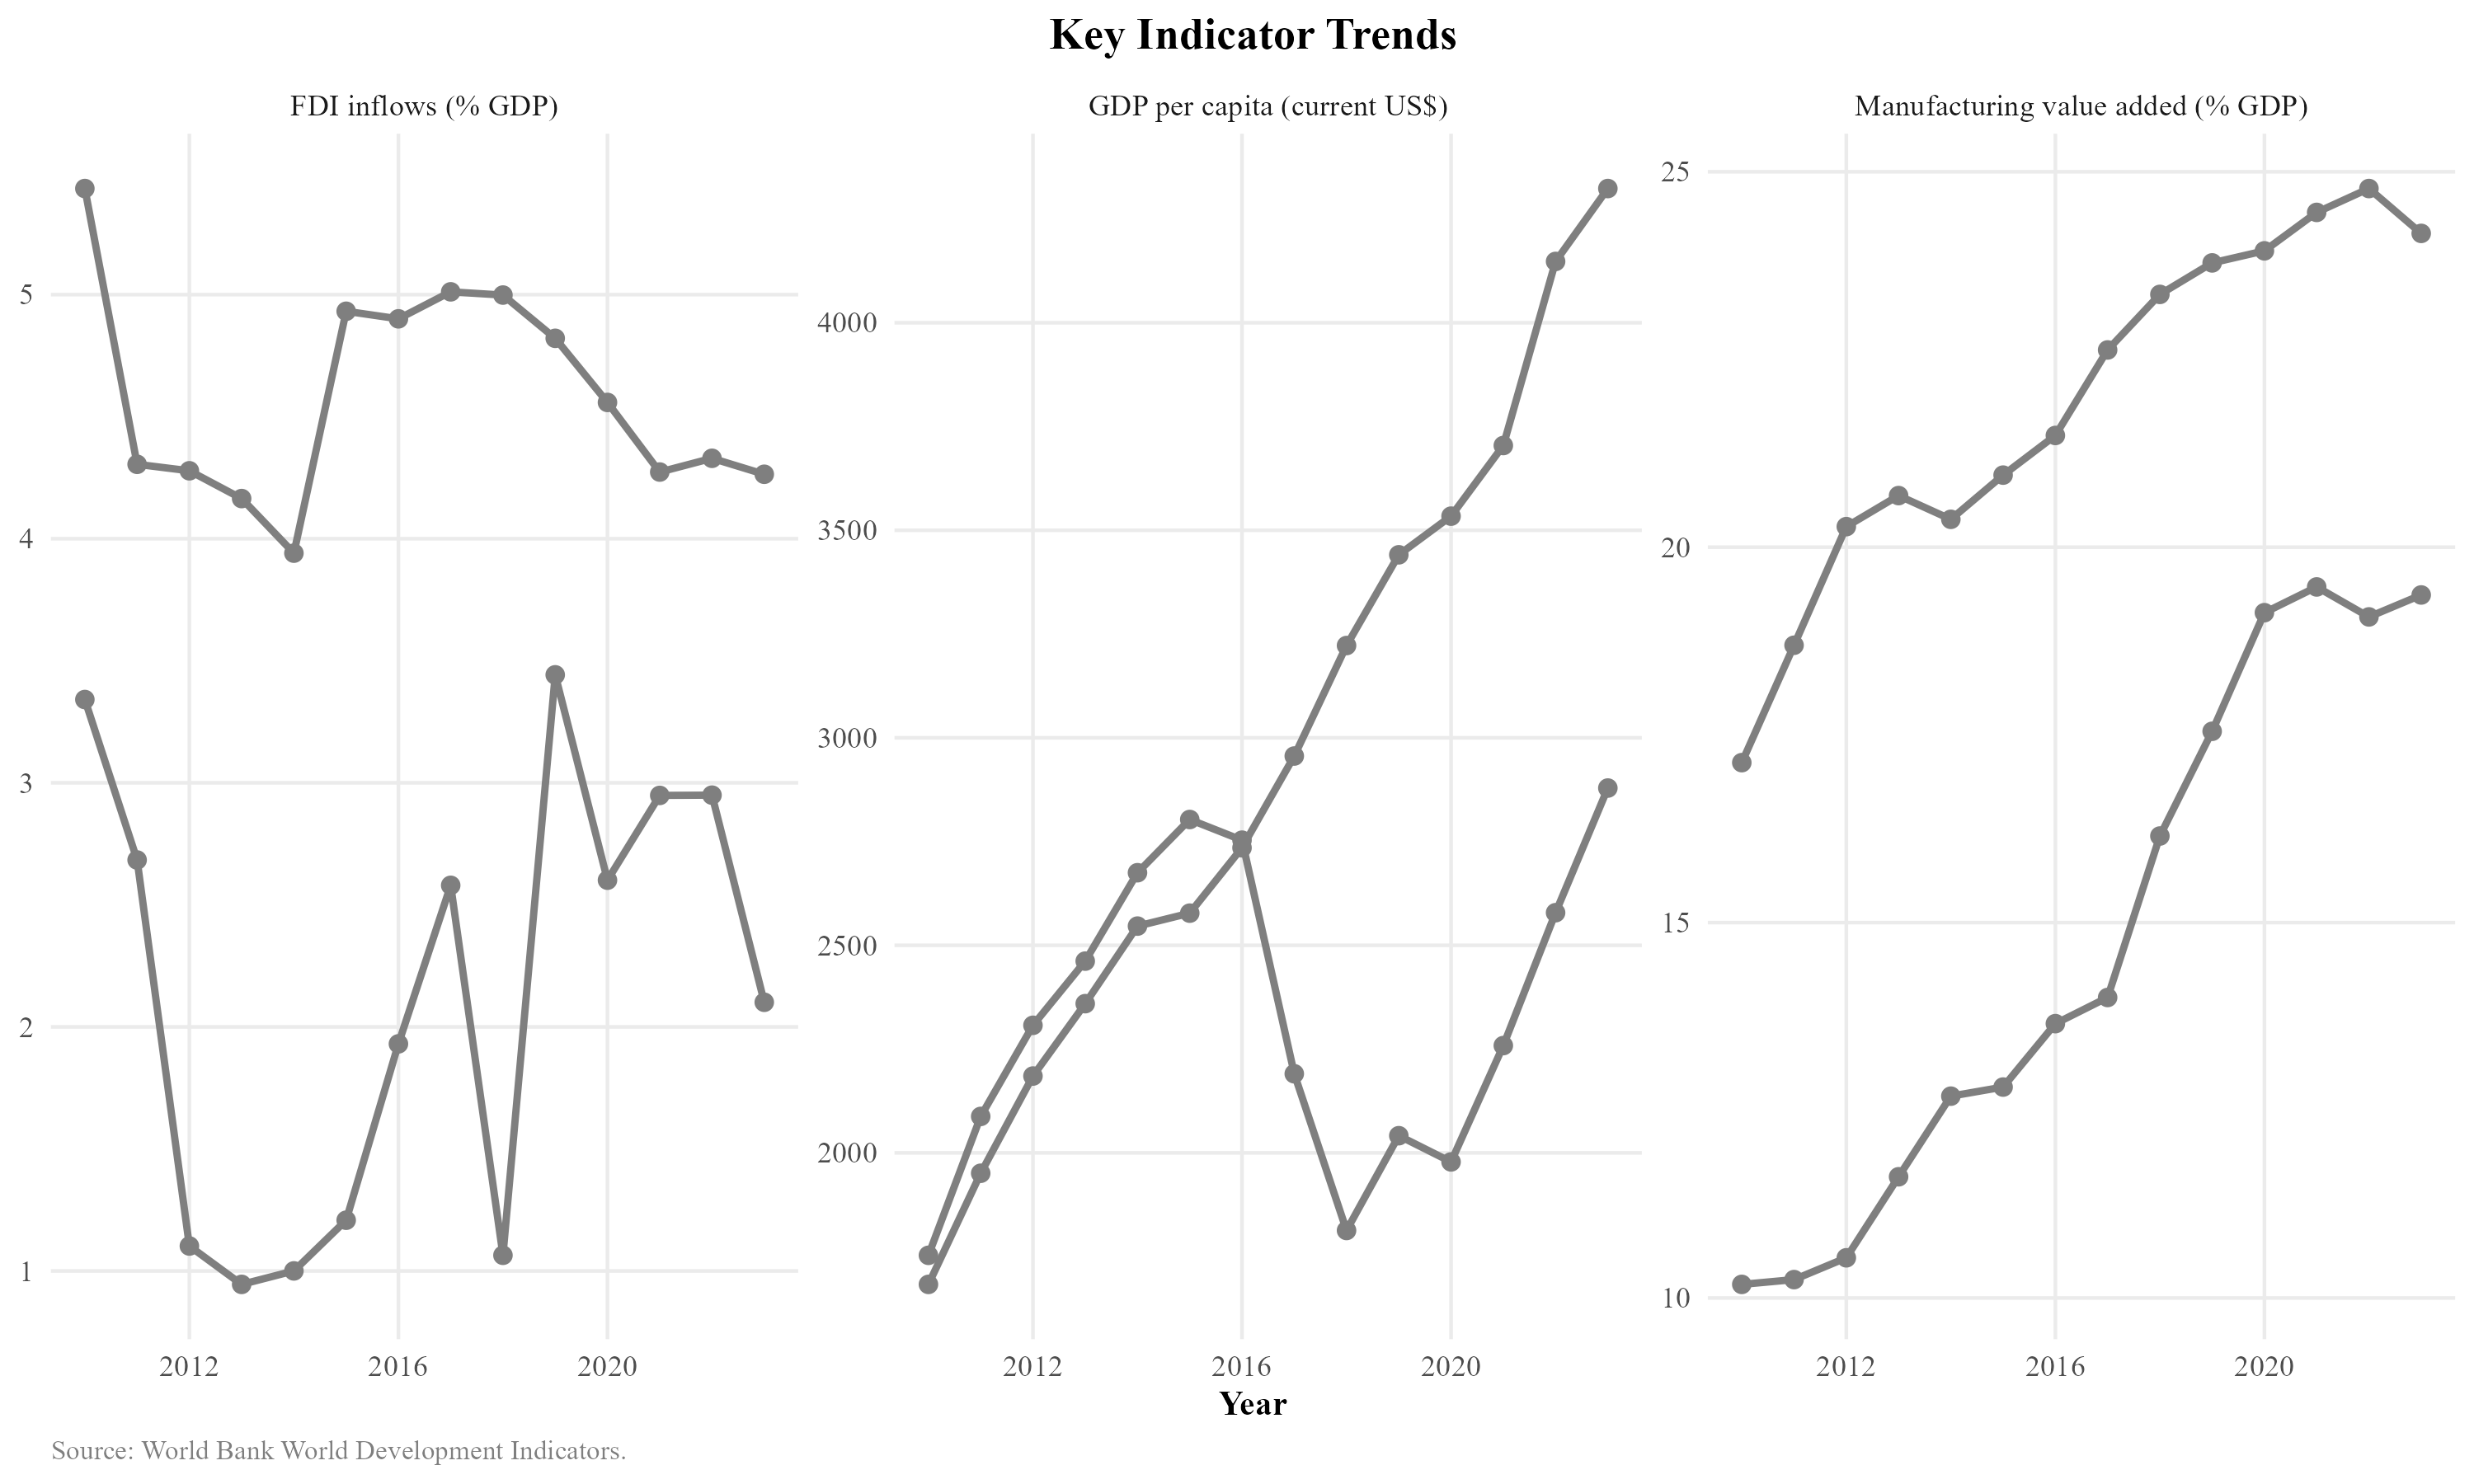
\includegraphics[width=0.90\textwidth]{figures/fig0_indicator_trends.png}
  \caption{Key Indicator Trends: FDI Inflows, GDP per Capita, and Manufacturing VA, Uzbekistan. Source: World Bank WDI.}
\end{figure}

\begin{figure}[H]
  \centering
  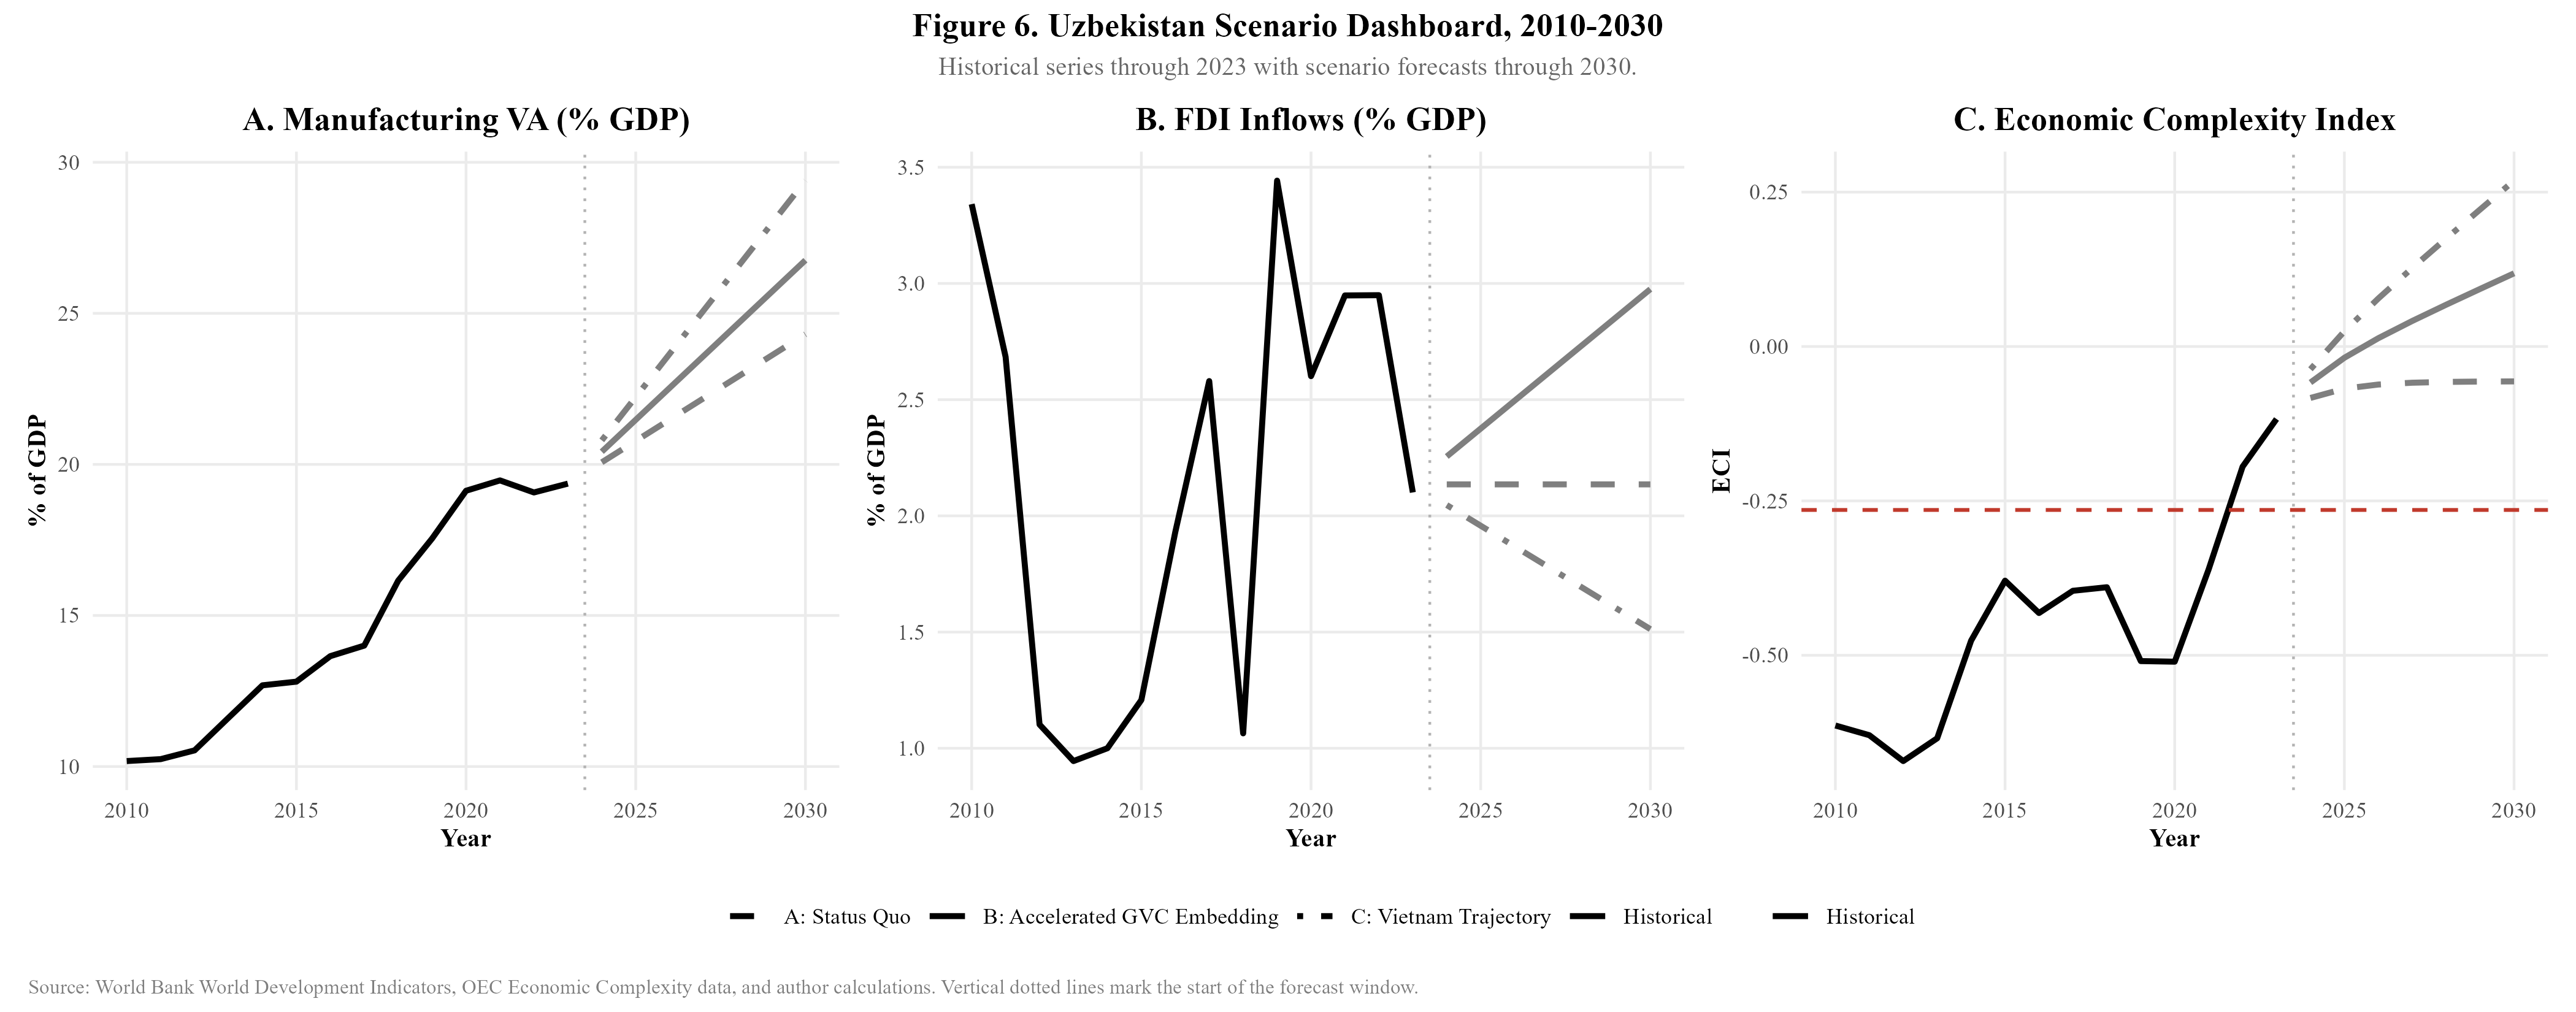
\includegraphics[width=0.90\textwidth]{figures/fig6_scenario_dashboard.png}
  \caption{Uzbekistan Scenario Dashboard, 2010--2030: Manufacturing VA, FDI, and Economic Complexity Index under three policy scenarios. Source: World Bank WDI, OEC, and author calculations.}
  \label{fig:scenario_dashboard}
\end{figure}

\begin{figure}[H]
  \centering
  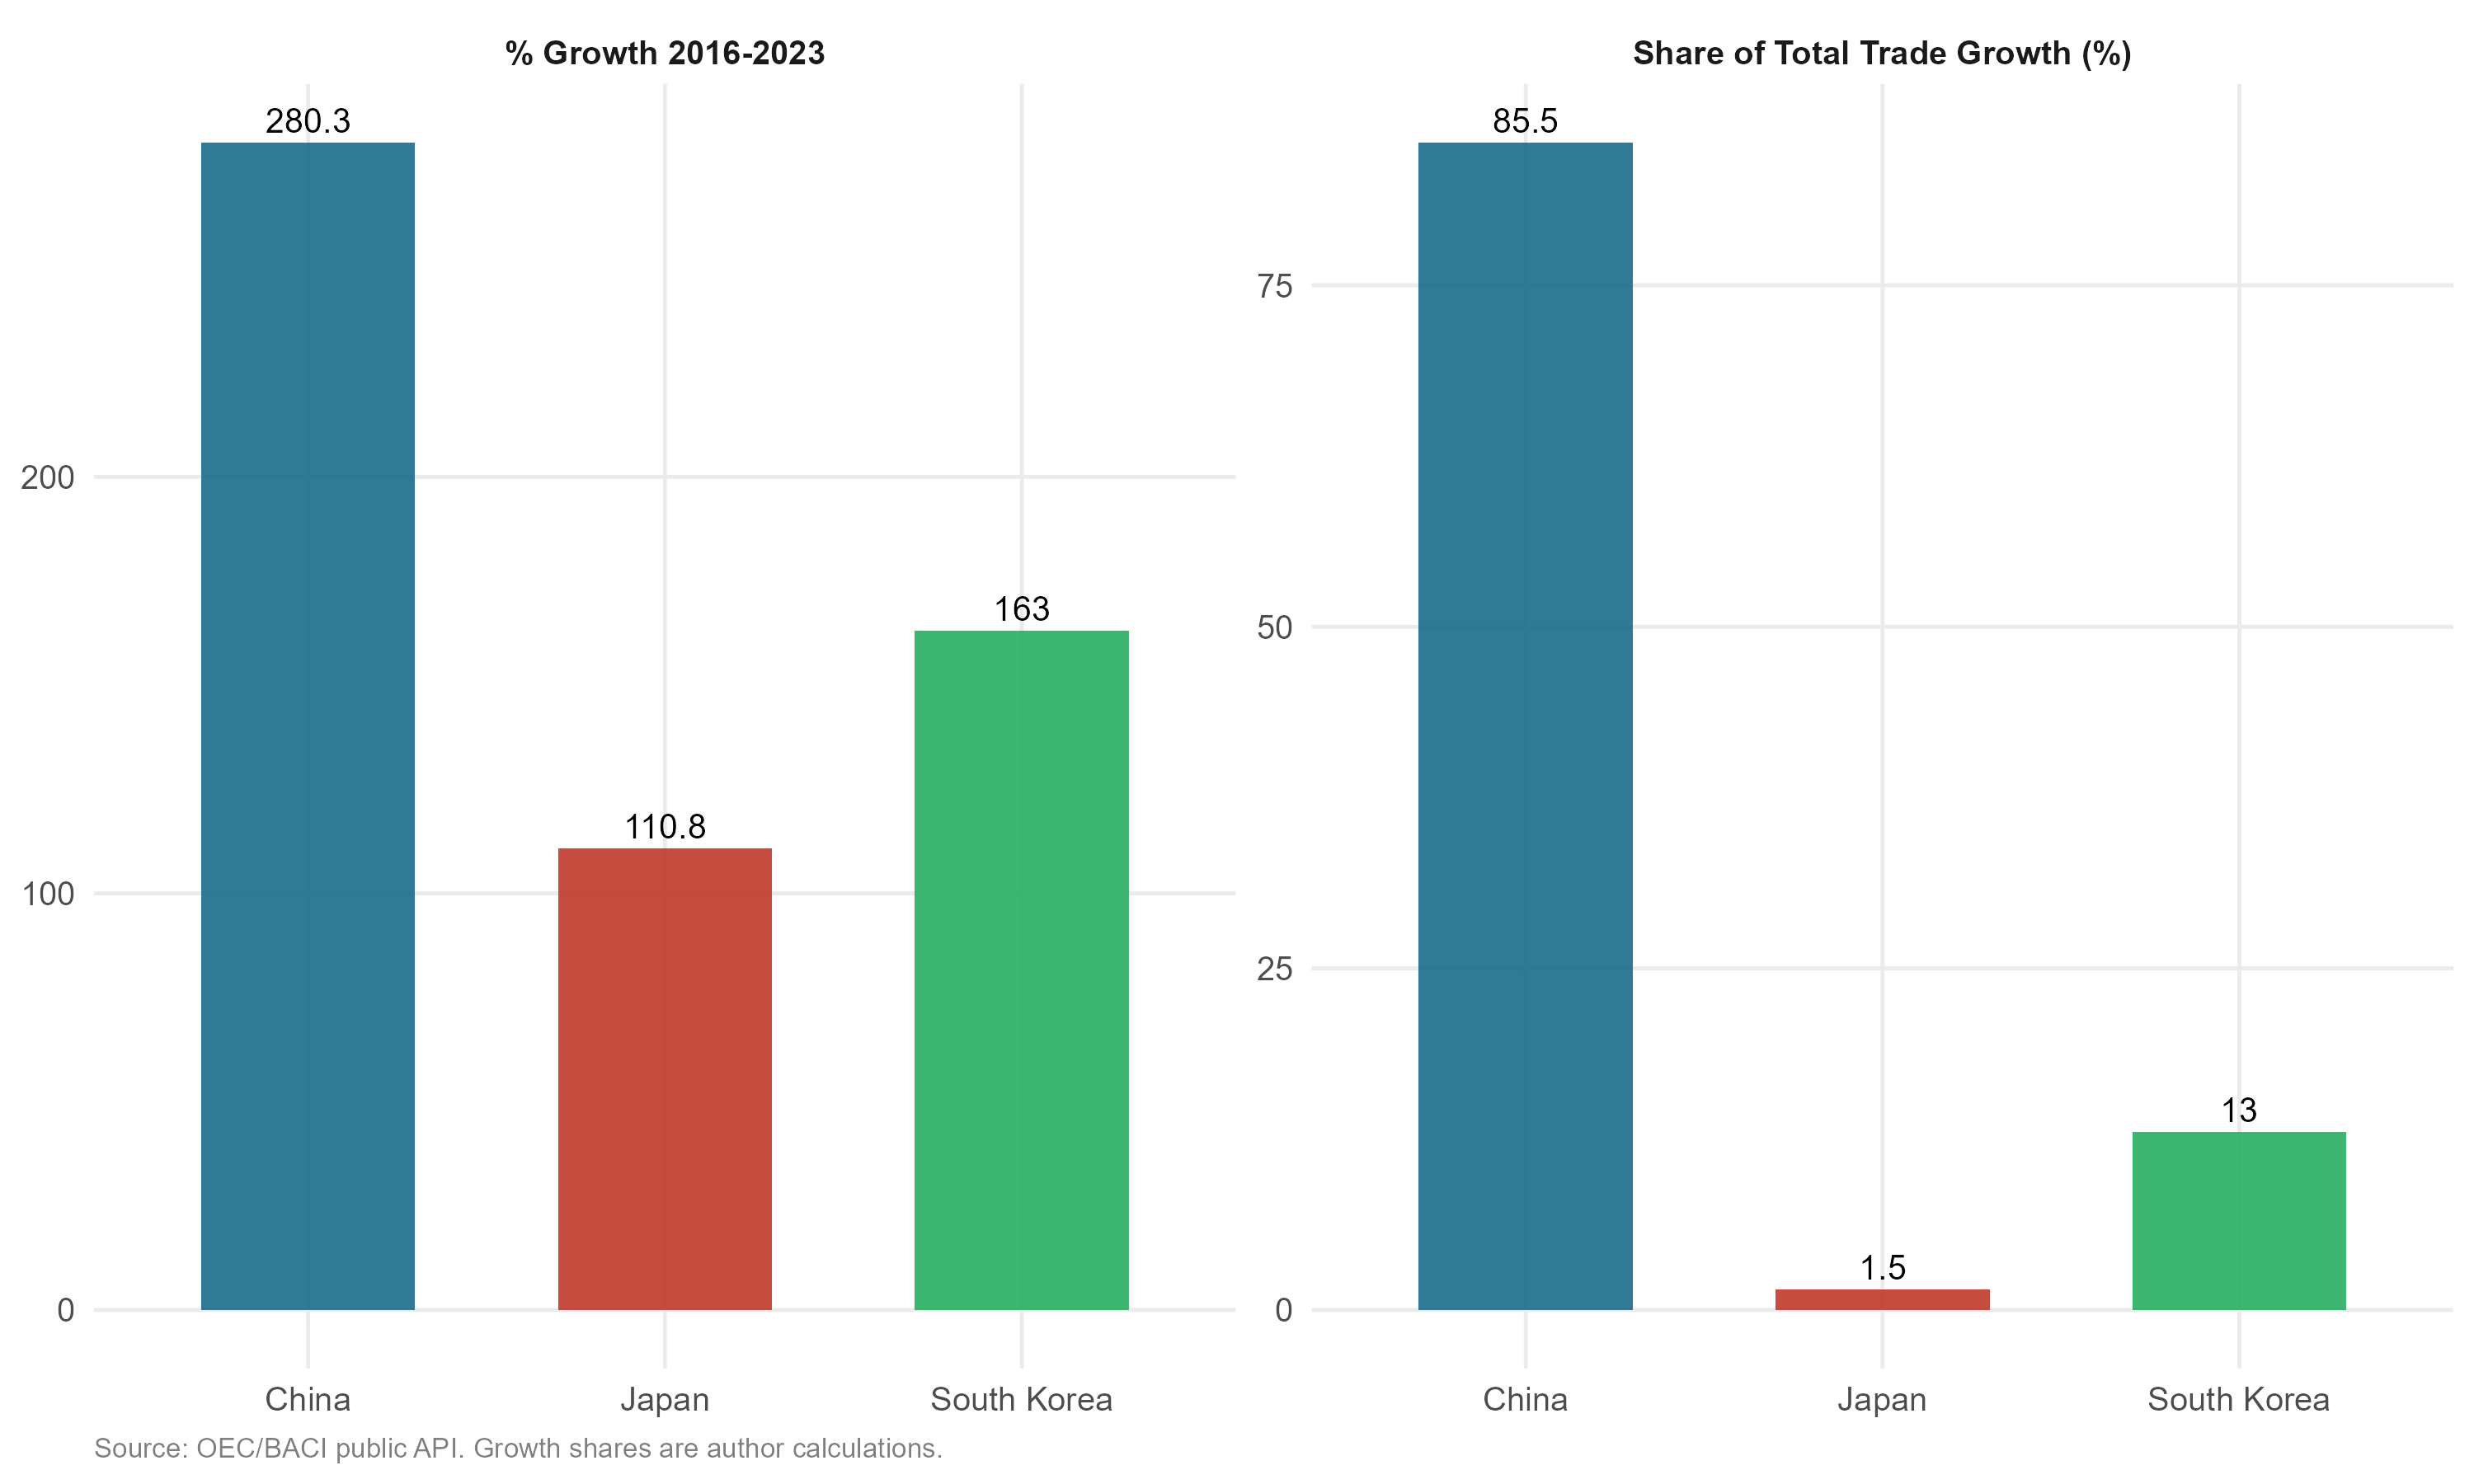
\includegraphics[width=0.90\textwidth]{figures/fig11_growth_decomposition.png}
  \caption{Post-Reform Trade Growth Decomposition by Northeast Asian Partner, 2016--2023. Source: OEC/BACI public API.}
\end{figure}

\end{appendices}

% ── REFERENCES ────────────────────────────────────────────────────────────────
\newpage
\bibliographystyle{agsm}

\bibliography{references_cleaned}

\end{document}
